\documentclass{report}
\usepackage[utf8]{inputenc}
\usepackage{hyperref}

\usepackage{amsmath}
\usepackage{amsfonts}
\usepackage{pdfpages}
\usepackage{graphicx}
\usepackage{geometry}
\usepackage{xcolor}
\usepackage{pdfpages}
\usepackage[some]{background}

\newcommand{\norm}[1]{\left\lVert#1\right\rVert} % Defines norm command
\newcommand{\abs}[1]{\lvert#1\rvert}

\usepackage{mathtools}
\DeclarePairedDelimiter\ceil{\lceil}{\rceil}
\DeclarePairedDelimiter\floor{\lfloor}{\rfloor}

\hypersetup{
    colorlinks=true,
    linkcolor=blue,
    filecolor=magenta,      
    urlcolor=blue,
}



\title{\huge \textbf{Robotics Research Center Summer School}}
\author{Jaidev Shriram}
\date{}

\usepackage{lipsum}

\definecolor{titlepagecolor}{cmyk}{1,.60,0,.40}

\backgroundsetup{
scale=1,
angle=0,
opacity=1,
contents={\begin{tikzpicture}[remember picture,overlay]
 \path [fill=titlepagecolor] (current page.west)rectangle (current page.north east); 
 \draw [color=white, very thick] (5,0)--(5,0.5\paperheight);
\end{tikzpicture}}
}

\makeatletter                   
\def\printauthor{%                  
    {\large \@author}}          
\makeatother

\author{%
    Jaidev Shriram \\
    IIIT-H \\
}

\begin{document}

\begin{titlepage}
\BgThispage
\newgeometry{left=1cm,right=6cm,bottom=2cm}
\vspace*{0.4\textheight}
\noindent
\textcolor{white}{\Huge\textbf{\textsf{Robotics Summer School Notes}}}
\vspace*{2cm}\par
\noindent
\begin{minipage}{0.35\linewidth}
    \begin{flushright}
        \printauthor
    \end{flushright}
\end{minipage} \hspace{15pt}
%
\begin{minipage}{0.02\linewidth}
    \rule{1pt}{175pt}
\end{minipage} \hspace{10pt}
%
\begin{minipage}{0.63\linewidth}
\vspace{5pt}
    \begin{abstract} 
This is a collection of notes and topics explored during the robotics summer school at the International Institute of Information Technology, Hyderabad. The school is essentially a crash course on mobile robotics, computer vision, and essential math that also explores research topics taught at RRC. The github repo for this session can be found \href{https://github.com/RoboticsIIITH/summer-sessions-2020}{here}.
    \end{abstract}
\end{minipage}
\end{titlepage}
\restoregeometry

\tableofcontents{}

\setlength{\parskip}{\baselineskip}%
\setlength{\parindent}{0pt}%

\part{Math Review}

\chapter{Linear Algebra Overview}

This chapter is critical to understanding the basics of what drives everything useful. This ranges from modelling problems and our data to processing them for deep learning, triangulation, and much more. In general, we can say that a robot has sensors, a CPU, and actuators. Each work with data and modelling this data is critical to processing it. For instance, the coordinate system used to represent objects could be cartesian, polar, etc.

\section{Vectors and Matrices}

Nothing new here. Vectors are single row/column matrices that represent a quantity. We will mostly be dealing with column vectors exclusively. Using vectors and matrices, we can model equations concisely. For instance,

\begin{equation*}
\begin{split}
    3u + 4v & = -6 \\
    9u - 5v &= 3
\end{split}
\end{equation*}

can be represented as $Ax = b$ where A is a matrix, and x, b are column vectors.

\begin{equation*}
    \begin{bmatrix}
    3 & 4 \\
    9 & -5
    \end{bmatrix} 
    \begin{bmatrix}
    u \\
    v
    \end{bmatrix}
    =
    \begin{bmatrix}
    -6 \\
    3
    \end{bmatrix}
\end{equation*}

Writing this in \LaTeX  is a pain and this information is trivial. Refer to the slides if this is confusing.

\section{Length of Vector}

There are various measures that represent the length of a vector. The norm is a function that lets us do this by taking a vector and returning a non-negative number. It satisfies few properties:

\begin{enumerate}
    \item Positivity: $\norm{x} >= 0$
    \item Definiteness: $\norm{x} = 0$ if and only if $x=0$
    \item Absolutely Homogenous: $\norm{\alpha x} = \abs{x} \norm{x}$
    \item Triangle Inequality: $\norm{x + y} \leq \norm{x} + \norm{y}$
\end{enumerate}

There are various norms that exist such as L2 norm (root of sum of squares), L1 norm (sum of absolute values), infinity norm and p-norm ($\norm{x}_p = (\abs{x_1}^p + \abs{x_2}^p + \cdots \abs{x_n}^p)^{1/p}$).

\section{Angle}

We can gauge orthogonality using inner product which is a generalization of dot product usually. It is a function that takes two vectors and returns a real number. It follows properties:

\begin{itemize}
    \item Positivity: $\langle x, x \rangle \geq 0$
    \item Definiteness: $\langle x, x \rangle = 0$ if and only if $x = 0$
    \item Additivity: $\langle x+y, z \rangle = \langle x, z \rangle + \langle y, z \rangle$
    \item Homogeneity: $\langle \lambda x, y \rangle = \lambda \langle x,y \rangle$
    \item Symmetry: $\langle x, y \rangle = \langle y, x \rangle$
\end{itemize}

\subsection{Dot Product}

The dot product of two vectors $x, y \epsilon \mathbb{R}^n$, is 
\begin{equation}
x \cdot y = \Sigma_{i=1}^{n} x_i y_i
\end{equation}

Orthogonal vectors satisfy $\langle x, y \rangle = 0$

We can use any other norm in a inner product space to measure lengths as well.

\section{Cross Product}

Given two vectors $x$ and $y$, the cross product $x \times y$ is a vector $z$ perpendicular to both $x$ and $y$ with a direction perpendicular to both vectors and direction given by right hand rule. 

This expression is commonly understood and won't be covered in depth.

\subsection{Equivalent Forms}

There are multiple ways to represent the cross product. The most popular one for computing utilizes matrices and computes cross product by multiplying matrices. Look at slide 14/43 in the lecture slides to see the formulation. It is using a skew symmetric matrix to calculate the cross product.

\section{Vector Space}

The vector space is a set of vectors that are closed under vector addition and scalar multiplication operations. Some operations possible with vectors are:

\begin{itemize}
    \item Vector Addition
    \item Scalar Multiplication
    \item Dot Product
    \item Cross Product
\end{itemize}

Remember the basic conditions of linear independence and span. Vector sets that satisfy both form the basis for a vector space. The dimension of a vector space is the cardinality of a basis.

\section{Matrix-Matrix \& Matrix-Vector Operations}

There is nothing special to this section but based on how we choose to look at the product, we can realize the operation in different ways. All these are equivalent. Look at the slides 17-19 for more.

Also look at slide 26 for an understanding of row space, null space, and how they relate to each other. It is quite interesting.

\section{Trace}

This is the sum of all diagonal elements in a matrix.

\section{Inverse}

You know what it is:

\begin{equation}
    AA^{-1} = A^{-1}A = I
\end{equation}

The inverse may not exist for all matrices and needs to meet some conditions.

\section{Rank}

The row and column rank are the largest subset of rows/columns that constitute a linearly independent set. Some interesting properties of row and column rank are:

\begin{itemize}
    \item row rank = column rank
    \item $rank(A) = rank(A^T)$
    \item $rank(A+B) \leq rank(A) + rank(B)$
    \item $rank(AB) \leq min(rank(A), rank(B))$
\end{itemize}

Inverse does not exist when A is not full rank.

\section{Miscellaneous Notes}

Slide 27 of the deck is a very new way of looking at determinant. Not yet understood entirely.

Frobenius norm is a commonly used norm: $\norm{A}_F = \sqrt{\Sigma_{i=1}^{m}\Sigma_{j=1}{n}\abs{a_{ij}}^2}$
Kronecker product is essentially the tensor product of two matrices.

\subsection{Role of orthogonal matrices}

Orthogonal matrices act as length preserving and angle preserving transformations. THey ensure that the dot product of two vectors remain the same before and after transformation. So, if we imagine an orthogonal transformation on a unit cube, then it essentially just creates a new unit cube. This isn't the case with all linear transforms obviously - which can stretch the cube, squash it to a square (parallelogram), or even a line - depending on the rank of the transform matrix. \href{http://www.math.lsa.umich.edu/~kesmith/OrthogonalTransformations2017.pdf}{These set of questions} offer some nice examples to get a hold of this quickly.

\section{Quadratic Forms}

Read more and write

\section{Matrix Decomposition}

A matrix decomposition is factoring a matrix such that it is represented as the product of multiple matrices. There are various matrix decompositions that exist. These are primarily done for ease of computation and optimization.

\subsection{Eigen Decomposition}

This decomposes a matrix into eigenvectors and eigenvalues. We know that an eigenvector, is a vector that satisfies $Av = \lambda v$. 

Now, we if have a series of equations of the form:

\begin{equation}
\begin{split}
    Ax_1 &= \lambda_1 x_1 \\
    Ax_2 &= \lambda_n x_2 \\
    &= \vdots \\
    Ax_n &= \lambda_n x_n \\
\end{split}
\end{equation}

This set of vectors $\{x_1, x_2, \cdots, x_n\}$ can be represented as a matrix with these vectors are column vectors. Let this matrix be $Q$. Then,

\begin{equation}
    AQ = Q\times diag(\lambda)
\end{equation}

where $diag(\lambda)$ is the matrix with eigenvalues in the diagonal. Hence, we can rewrite this matrix as:

\begin{equation}
    A = Q \times diag(\lambda) \times Q^{-1}
\end{equation}

\subsection{Singular Value Decomposition (SVD)}

Any real $m\times n$ matrix $A$ can be uniquely decomposed as:

\begin{equation}
    A = UDV^T
\end{equation}

Here, $A$ is a matrix with $x_i$ as it's column vectors.

\href{https://www.youtube.com/watch?v=nbBvuuNVfco}{This} video is a great reference to see the intuition behind this decomposition and what each of the entities in the decomposition refer to.

$U$ can essentially be seen as the eigen series of the quantities measured in column vectors of $A$. The $\Sigma$ variable is the scaling and has an ordering. Hence, values that can cause more variance come first, heirarchically arranged. This arrangement corresponds to $U$ as well. The matrix $V^T$ has columns that represent what mixture of the product of previous two matrices can result in the original $x_i$ vector represented in A back. 

A detailed look at the SVD procedure and usecases can be found \href{https://www.cse.unr.edu/~bebis/MathMethods/SVD/lecture.pdf}{here}.

SVD is extremely useful in several scenarios. One intuitive usecase is in image compression. We know that SVD gives an ordering of singular values. To compress an image, we can delete the low importance onces entirely, reducing the dimension of an image. It also has applications in regression and modelling where it can help minimize certain function such as total least squares.

That said, the above explanation isn't enough to see how SVD works. \href{http://www.ams.org/publicoutreach/feature-column/fcarc-svd}{This} is a good resource with baby hand holding explanations.

As shown in the SMAI course, one beautiful thing about SVD is its ability to capture latent space. Or rather, hidden features. In the image example, we showed that we can choose the most important features - we never tell it WHAT features exist. \href{https://sifter.org/~simon/journal/20061211.html}{As this amazing resources explains}, SVD can help find hidden features which can help in recommender systems, or even in text modelling (finding keywords/topics of a document). Netflix uses SVD to make recommender systems in fact, predicting the rating a user would give a movie that he/she hasn't seen yet.

\subsection{Lower-Upper Decomposition}

In LU decomposition, we express a matrix $A$ as follows:

\begin{equation}
    A = LU
\end{equation}

where $L$ is a lower triangular matrix and U is an upper triangular matrix. This is essentially the matrix form of gaussian elimination. As per wikipedia "Computers usually solve square systems of linear equations using LU decomposition, and it is also a key step when inverting a matrix or computing the determinant of a matrix".

\subsection{QR Decomposition}

The QR decomposition is factorizing a matrix into an orthogonal matrix and triangular matrix such that:

\begin{equation}
    A = QR
\end{equation}

where Q is orthogonal and R is upper triangular.

A popular way to calculate this is to use the  Gram–Schmidt procedure, which finds an orthogonal basis from a set of vectors by removing the projection of a vector on the remaining iteratively.

\subsection{Cholesky Decomposition}

This is a decomposition of a positive definite square matrix into the product of a lower triangular matrix and it's transpose. In general,

\begin{equation}
    A = LL^*
\end{equation}

where L is the lower triangular matrix with real and positive diagonal entries. This decomposition is possible for every positive definite matrix and has a unique decomposition.

This decomposition is primarily useful for solving linear equations and in Kalman filters.

\chapter{Calculus Review}

This is part of the second lecture of the summer school series.

In linear algebra, we wanted to write all our information in the form of matrices. But linear algebra, restricts us to systems and functions to linear only. This assumption isn't always possible and hence, to represent other quantities such as polynomial path, a non linear curve on which we need to establish stability, we need to use non linear function. It is also important that we use something that the computer can use the non linear data, and with approximations among other things, get answers to our problems.

In general, if we have a function $f(x$, can we linearize it? If we could, then we could represent it in the matrix form

\section{Gradient}

Gradient can be defined as 

\begin{equation}
    f'(x) = \lim_{h \to 0} \frac{f(x+h) - f(x)}{h}
\end{equation}

But, this is single variable. If we have multiple variables, we can represent the gradient with respect to any of the variables.

\begin{equation}
    \frac{\partial f(x_1, x_2, ... x_n)}{\partial x_1} = \lim_{h_1 \to 0} \frac{f(x_1 + h, x_2, x_3, \cdots x_n) - f(x_1, x_2, \cdots x_n)}{h_1}
\end{equation}

Similarly, we can calculate the gradient for the remaining elements of x.

The slope is essentially the tangent to a curve. Hence, by taking a gradient, we are essentially linearizing by creating a line when we take derivative with a variable.

Here the input can be a vector, and let the function $f$ be one that gives us a scalar output. 

\begin{equation}
\nabla f =
\begin{bmatrix}
\frac{\partial f}{\partial x_1} \\
\frac{\partial f}{\partial x_2} \\
\vdots \\
\frac{\partial f}{\partial x_n}
\end{bmatrix}
\end{equation}

\href{https://atmos.washington.edu/~dennis/MatrixCalculus.pdf}{These notes} have a lot of examples of gradients involving matrices. Some of these questions were asked in the deep learning assignment. Computing derivatives of matrices is often unintuitive. In fact, even doing the math is tedious.

\section{Jacobian}

Now suppose that we have a function $f: R^N \to R^M$, takes a vector as input and produces a vector as output. Let the inputs be $\{ x_1, x_2, \cdots, x_n  \}$ and output be $\{ y_1, y_2, \cdots, y_m\}$. Then the derivative of $f$ at a point $x$, also called Jacobian is the $M \times N$ vector:

\begin{equation}
    J = \begin{bmatrix}
    \frac{\partial y_1}{\partial x_1} & \hdots & \frac{\partial y_1}{\partial x_n} \\
    \frac{\partial y_2}{\partial x_1} & \hdots & \frac{\partial y_2}{\partial x_n} \\
    \vdots & \ddots & \vdots \\
    \frac{\partial y_m}{\partial x_1} & \hdots & \frac{\partial y_m}{\partial x_n} \\
    \end{bmatrix}
\end{equation}

\subsection{Generalized Jacobian}

Just as a vector is a one-dimensional list of numbers and a matrix a two-dimensional grid of numbers, a tensor is a D-dimensional grid of numbers. Many operations in deep learning accept tensors as inputs and produce tensors as outputs. For instance, an image is usually represented as a three dimensional grid of numbers - height, width, and colour channels of the image. 

There is a lot of math here - nothing too fancy to understand. Refer to slides 12+ \href{https://github.com/RoboticsIIITH/summer-sessions-2020/blob/master/lecture-slides/deep_learning/vector_derivatives.pdf}{here}.

\textbf{There are some examples of derivatives \href{https://github.com/RoboticsIIITH/summer-sessions-2020/blob/master/lecture-slides/deep_learning/vector_derivatives.pdf}{here}}.

\section{Hessian}

Hessian of a function that is of the form $f: R^n \to R$, 

\begin{equation}
    \nabla^2 f = H = \begin{bmatrix}
    \frac{\partial^2 f}{\partial x_1^2} & \frac{\partial^2 f}{\partial x_1 \partial x_2} & \hdots & \frac{\partial^2 f}{\partial x_1 \partial x_n} \\
    \frac{\partial^2 f}{\partial x_1 \partial x_2} & \frac{\partial^2 f}{\partial x_2^2} & \hdots & \frac{\partial^2 f}{\partial x_2 \partial x_n} \\
    \vdots & \vdots & \ddots & \vdots \\
    \frac{\partial^2 f}{\partial x_1 \partial x_n} & \frac{\partial^2 f}{\partial x_2 \partial x_n} & \hdots & \frac{\partial^2 f}{\partial x_n^2} \\
    \end{bmatrix}
\end{equation}

This is a symmetric matrix.

\section{Model and Error}

How can we use the hessian and gradient? The reason for using this math is to model real data, and have some measure of quantities in the environment through sensors.

\begin{equation}
    X = f(P) \text{ in an ideal scenario}
\end{equation}

Now, we need to find parameters that can give the best result to measure the environment, or minimize the error. This function $f(P)$ need not be linear. This is where we need to use gradient and hessian.

\begin{equation}
    \norm{f(\hat{P}) - X} \text{ is to be minimized}
\end{equation}

\section{Linear Equations}

Sometimes, we can represent some sensors as linear models. We can use linear methods or decomposition methods to get a better reading from the model.

\begin{equation}
    f(P) = AP
\end{equation}

Here $A\; \epsilon R^{m \times n} \text{ and } P\; \epsilon R^n$. There are three cases:

\begin{itemize}
    \item $m < n$, we have many solutions. They form a vector space.
    \item $m = n$, we have either a unique solution or no solution.
    \item $m > n$, we have either a unique solution or no solution.
\end{itemize}

\textbf{No Solution case}

This happens when $b$ doesn't lie in the column space of A. If we don't have any solutions that are possible from the linear set of equations, we try to compute a vector that is close to the optimum.

\section{Non-Linear}

If we do not have a linear model, we need to find vector that fits the measurement data well.

\subsection{Taylor Series}

This is one approximation of a non linear function:

\begin{equation}
    f(x) = f(a) + \frac{f'(a)}{1!}(x-a) + \frac{f''(a)}{2!}(x-a)^2 + \frac{f'''(a)}{3!}(x-a)^3 + \cdots
\end{equation}

This is essentially a weighted sum.

If we have more variables, then we need to use a variant. We've already seen how we can use hessian and now for taylor series,

\begin{equation}
    f(x) = f(a) + \frac{\nabla f(a)^T}{1!}(x-a) + \frac{(x-a)^T \nabla^2f(a)(x-a)}{2!} +  \cdots
\end{equation}

Note that the transpose here is since they are all column vectors. By taking transpose, we can essentially take dot product. All the terms in the above expression are a vector, as opposed to the scalars in the single variate form. Most of the times, the first and second order approximation is enough. 

\begin{equation}
    Accuracy equations
\end{equation}

Using higher order estimations, only increase the accuracy of the estimate. 

\subsection{Cost Function}

We start with an initial estimate $P=P_0$ and we can use Taylor series to approximate cost function. We have an approximation of the cost at $P_0$. Now, we have a change of $\delta P$, then we can approximate cost of the new estimate.

\textbf{Most of this section is visited in detail in the SLAM: Optimization chapter.}

\subsubsection{First Order Method}

This method is called gradient descent. Now, if we take gradient with respect to parameter $P$, it is called Jacobian.

This is an iterative approximation and at every step, we decide what direction to take derivative in and how we can descent

\section{Contour line and Vector Field}

Now, if we take gradient along all possible values that we can take, then we get a vector field. 

Levengerg Marquardt - tends to converge to global minima. Will be used extensively.

During gradient descent, we may tend to miss the direction that will lead to minimum. It may be slower. Used for bundle adjustment.

In general, gradient descent is minimize f(x).

We can also have constraints. For a robot, if we want it to pass through some way points while being at some distance from an obstacle. Here, we have to minimize the function and subject it to certain constraints. 

Now, if we have a constrained problem, how do we solve it? The previous methods did not consider any constraints.

$h_i$ can be considered to be a constraint and we can have weight ages to constraints as well. Hence, there is more penalty for violating a constraint and so on.

Lagrange multiplier can be seen as a smooth approximation to $I_0$. The key idea with this is that by adding a new variable, we are able to convert constrained to unconstrained problem.

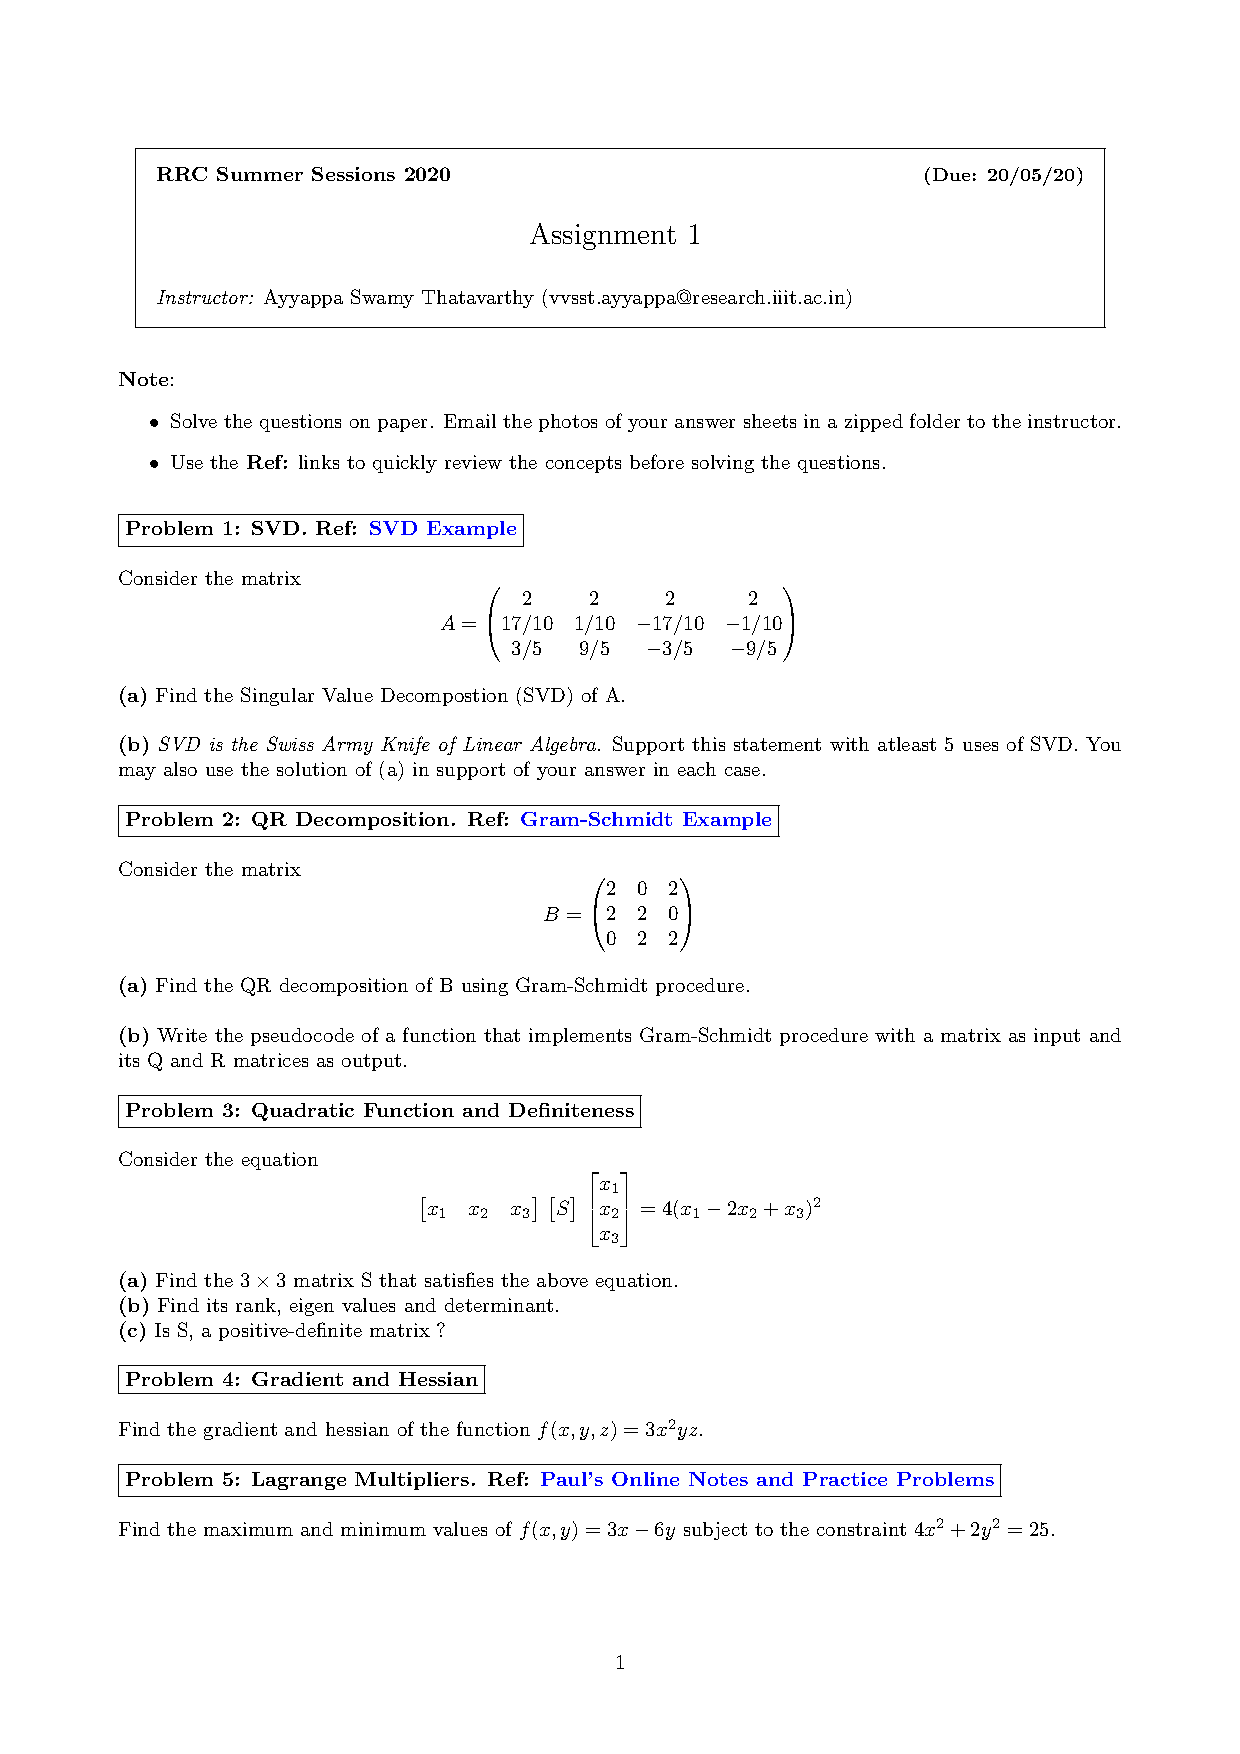
\includepdf[pages=-]{./Assignments/Assignment1.pdf}

\part{Deep Learning}

\chapter{Introduction to Machine Learning}

As per Tom Mitchell, machine learning is a new form of computer program that can learn from an experience with respect to some class of tasks, with a performance measure.

There are a few categories of ML:

\begin{itemize}
    \item Supervized Learning: Labeled data (input and output pairs exist). The machine learning model will be able to predict the output when given a set of inputs. Example, in linear regression, we have the input set and know the range of the output.
    \item Unsupervized Learning: There are no labels/targets for this data. Hence, we do not know what the output it supposed to be. Here, we essentially try to learn some patterns or features for this set of data. A common task is clustering various points (the number of clusters may not be evident either).
    \item Reinforcement Learning: Here, it's not like the previous two but has elements of both. In RL, there is an action, a state, a reward, and an environment. For instance, a robot can take an action which affects the environment, changing the state and gains a reward for this sequence. The purpose of the RL agent is to decide the actions (from a defined space) to optimize the rewards received. For an object avoiding robot, we can imagine that the cost of colliding or reward is negative (not desirable). More on this will be covered later.
\end{itemize}

There are more such as semi-supervised but they will not be discussed.

\section{Supervised Learning}

There is a training dataset which is pre-labelled. The ML algorithm is required to come up with a hypothesis function that can add labels to an unlabeled input. Essentially, we need a function $f(x) = y$ where x is the input features and y is the output we want to predict. This function should model the training data well and model unseen data well too. 

\subsection{Classification}

In classification, the hypothesis function is defined as $h: x \to y$, where $x \epsilon R^m$ and $y \epsilon \{0,1,\cdots ,k\}$

\subsection{Regression}

In regression, the hypothesis function maps input to a continuous output range. Example: Stock market prediction.

\section{Hypothesis Space}
The hypothesis space can usually be extremely large, and often infinitely large. For instance, an integer domain. 


\section{Neural Networks at a glance}
A neural network with a single hidden layer, a finite number of neurons and non-linear activation functions such as sigmoid units was proved to be a universal function approximator. These are some of the most useful machine learning algorithms. Obviously, a single layer is not very useful for modelling but this can be explored in more depth later. If you want, watch 3Blue1Brown's videos on neural networks.

\section{Model Selection}

There are typically two datasets - train and test. The training set is the data that we use to train the ML Algorithm. The test data is meant to mimic how the model will perform in real life. It is an unseen set of data that can gauge how good the model is. We also use a validation set for similar reasons.

\textbf{True error rate}: The classifier error on the ENTIRE population. This is nearly impossible to determine but estimates can be made.

We have error rate in the training set. For instance, 95\% accuracy in training data means that with 95\% data we can predict our output. True error data is not limited by the train or test data but rather the entire sample space.

\subsection{Holdout Method}

We can split the dataset into two groups - training and test. We can keep adding data to the training data, and test on test data until the test error is satisfactory

\textbf{Epochs vs Mean Square Error}: Epochs are the number of iterations on which it is trained. Once we find a minimum error for the test data after plotting it, we can stop. Increasing the epochs risks over fitting since it learns too much from the training set.

\section{K-Fold Cross Validation}

We create K-Fold partitions of the dataset. For each each of the K experiments, we use K-1 folds for training and remaining set for the training. The true error here is \textbf{estimated} as the average error rate across all experiments. 

\subsection{No of Folds}

With large number of folds, the bias of true error estimator will be small - more accurate. The variance of the true error will also be large. Additionally, the computational time will be large as well.

With small number of folds, the computational time may be reduced and variance may be small but bias will be larger. The training set size will have reduced quite a bit and in Deep Learning we want size of training data to be high. 

For large datasets, even 3-Fold Cross Validation is accurate enough. Sometimes, 5-Fold Cross validations is common too. For very sparse datasets, we may have to use leave-one-out in order to train on as many examples as possible. 

\section{Hyper parameters}

Across various machine learning methods, there are various parameters that can be tweaked. From our previous examples, it could be number of layers in the neural network or choice of folds. These hyper parameters should NEVER be based on the test set - as they are meant to be reflections of real life. Otherwise, overfitting on test set is also possible. 

We can choose our hyperparameters by training and then validating performance on a validation test. And, we can finally test on the test set.

\section{Bias-Variance Tradeoff}

\begin{center}
    \textbf{Total Error = Bias + Variance + Irreducible Error}
\end{center}

Even a perfect model will not be able to reduce all the errors as the training data itself may contain noise. This, we try to reduce the bias and variance as much as possible. Hence, it's nearly impossible to get 100\% accuracy in a dataset. If we do get 100\%accuracy then the dataset is too simple. 

\subsection{Bias}

The difference between the average prediction of our model and correct value. In regression, it is the square of the difference. Model with high bias is indicative of oversimplification in the model and leads to high error in the training and test error.

\subsection{Variance}

Variance is the variability of model prediction for a given data point which tells us spreads of our data. Basically, on changing the input, how much does the output get affected. A model with high variance doesn't generalize very well on unseen data. 

We ideally want low bias and low variance but this is easier said than done. It has been found that as model complexity increases, the bias reduces but variance increases. This is the tradeoff between the two. We can measure for these errors in K-Fold Cross validation to minimize both.

\section{Overfitting and Underfitting}

Underfitting happens when the model is too simple and is unable to capture the underlying patterns of the data. It usually has high bias and low variance - it is bad predictor and is consistently bad (hence low variance)

Overfitting happens when the model captures too much of the noise as well. It usually has low bias as a result but high variance.

\section{Maximum Likelihood Estimation (MLE) and Maximum A Posteriori (MAP)}

MLE and MAP are both methods of estimating some variable in the setting of probability distributions or graphical models.

\subsection{MLE}

\href{https://www.probabilitycourse.com/chapter8/8_2_3_max_likelihood_estimation.php}{This} is a great resource for reading up about MLE. As per \href{https://towardsdatascience.com/probability-concepts-explained-maximum-likelihood-estimation-c7b4342fdbb1}{another great article}, "Maximum likelihood estimation is a method that determines values for the parameters of a model. The parameter values are found such that they maximise the likelihood that the process described by the model produced the data that were actually observed." This is the best way to understand the importance of MLE in ML.

In \textbf{MLE}, we choose $\theta$ that maximizes the probability of observed data.

Here, we are trying to find the value $\theta$ that estimates the data best.

\textbf{Why is this relevant?}

Most of the optimization in CNN, or NN in general we want to find the best parameters using MLE.

Let the likelihood function be $P(X|\theta)$. The, the MLE for $\theta$ is:

\begin{equation}
\begin{split}
    \theta_{MLE} &= arg_{\theta} \; maxP(X|\theta) \\
    &= arg_{\theta} \; max \; \Pi_{i} P(x_i | \theta)
\end{split}
\end{equation}

We generally do not tend to use this since the number can become 0 quickly as numbers go to infinity. Hence, we tend to use the logarithm and try to minimize that:

\begin{equation}
\begin{split}
    \theta_{MLE} &= arg_{\theta} \; max \log P(X|\theta) \\
    &= arg_{\theta}\; max \; \log \Pi_{i} P(x_i | \theta) \\
    &= arg_{\theta}\; max \; \Sigma_i \log P(x_i | \theta)
\end{split}
\end{equation}

The two functions are equivalent since the logarithm is monotonically increasing, and hence can be used.

\subsection{MLE for Gaussian}

\textit{A Gaussian or normal distribution is one which is symmetric about the mean and peaks at the mean value. Read up if confused.}

The parameters for a Gaussian distribution are the mean ($\mu$) and variance ($\sigma^2$). When fitting a Gaussian to our dataset, we take the sample mean and variance of the dataset and use that as parameter for the Gaussian. 

Given observations $x_1, x_2, \cdots, x_N$ the likelihood of those observations for a certain $\mu$ and $\sigma^2$ is:

\begin{equation}
    P(x_1, \cdots, x_N | \mu, \sigma^2) = \Pi_{n=1}^{N} \; \frac{1}{\sigma\sqrt{2\pi}} \: exp\{\frac{-(x_n-\mu)^2}{2\sigma^2}\}
\end{equation}

The log likelihood for the same is:

\begin{equation}
    L(\mu, \sigma) = -\frac{1}{2}N\log(2\pi \sigma^2) - \Sigma_{n=1}^{N} \frac{(x_n - \mu)^2}{2\sigma^2}
\end{equation}

But, the sigma (variance) that we get from MLE is a biased estimator. In statistics, we evaluate the “goodness” of the estimation by checking if the estimation is “unbi-ased”. By saying “unbiased”, it means the expectation of the estimator equals to the true value, e.g.if $E[x] = \mu$ then the mean estimator is unbiased as per \href{https://dawenl.github.io/files/mle_biased.pdf}{this}. \href{https://stats.stackexchange.com/questions/136673/how-to-understand-that-mle-of-variance-is-biased-in-a-gaussian-distribution}{This} stack overflow answer has a great explanation as to why the variance is biased.

"The intuition is that in a non-squared sample mean, sometimes we miss the true value $\mu$ by over-estimating and sometimes by under-estimating. But, without squaring, the tendency to over-estimate and under-estimate will cancel each other out. However, when we square $\bar{x}$ the tendency to under-estimate (miss the true value of $\mu$ by a negative number) also gets squared and thus becomes positive. Thus, it no longer cancels out and there is a slight tendency to over-estimate.
 
\subsection{MAP}

The MAP estimate of a random variable $X$, given that we have observed $Y = y$ is given by the value of x that maximizes $P_{X|Y}(x|y)$.

\href{https://www.probabilitycourse.com/chapter9/9_1_2_MAP_estimation.php}{This} is a reference from the probability course about MAP estimation. It is decent and has a few examples that explain the concept.

MAP usually comes up in a Bayesian setting where we work on a posterior distribution, not \textbf{only} the likelihood. So usually, for:

\begin{equation}
\begin{split}
    P(\theta | X) &= \frac{P(X|\theta)P(\theta)}{P(X)} \\
    &\alpha \; P(X|\theta)P(\theta)
\end{split}
\end{equation}

We are ignoring the normalizing constant as proportionality is sufficient.

Let's assume that we have a classifier for cats and dogs. If we know the general distribution of dogs and cats in the world, we can feed that ratio to the model and this is prior information. In general, this prior is expert knowledge.

\begin{equation}
\begin{split}
    \theta_{MAP} &= arg_{\theta}\; maxP(X|\theta)P(\theta) \\
    &= arg_{\theta}\; max \log P(X|\theta) + \log P(\theta) \\
    &= arg_{\theta}\; max \log \Pi_i P(x_i|\theta) + \log P(\theta)\\
    &= arg_{\theta}\; max \; \Sigma_i \log P(x_i|\theta) + \log P(\theta)
\end{split}
\end{equation}

Comparing MLE and MAP, the only thing that differs is the inclusion of prior in MAP. Hence, for a uniform prior, the MAP is same as MLE. If we take derivative of the distribution, it will be 0 since it won't change. Note that we are trying to maximize the function here for all values of theta. So, derivative is taken to reach the optima using a method such as gradient descent. \href{https://wiseodd.github.io/techblog/2017/01/01/mle-vs-map/}{This} is a good resource that differentiates and connects between MLE and MAP.

"If we use different prior, say, a Gaussian, then our prior is not constant anymore, as depending on the region of the distribution, the probability is high or low, never always the same.

What we could conclude then, is that MLE is a special case of MAP, where the prior is uniform!"

Most of the CNN approaches may use MLE but other algorithms exist which use MAP. 

\chapter{Regression}

As with anything ML related, the Andrew NG course will help - and material from this was used to teach this topic.

In regression, we have a continuous range or set of labels that we try to predict. There are various degrees of functions that we can try using to model the data such as linear or quadratic.

Our features for a regression could be continuous, binary, or something else entirely too. Regression is primarily concerned with the range not the domain.

Input data could be weight and height of a person, making input a $R^2$ vector. \[ X = \{x^1, \cdots, x^n\} \text{ where } x^i \epsilon R^d \]

\section{Linear Regression}

A general linear regression hypothesis looks like:

\begin{equation}
    y \; = \; \theta_0 + \theta_1x_1 + \theta_2x_2 + \cdots + \theta_dx_d = \Sigma_{j=0}^{d} \; \theta_jx_j
\end{equation}

Hence, we have $d+1$ parameters to determine since the input has $d$ features and we have another constant (is like a bias).

The error is usually the L2 norm or sum of the squares of difference from the best fit line values. The cost function is:

\begin{equation}
    J(\theta) = \frac{1}{2n} \: \Sigma_{i=1}^{n} (h_{\theta} (x^{(i)} - y^{(i)})^2
\end{equation}

We need the cost function for the machine learning algorithm to optimize the accuracy of the model. The $\frac{1}{2n}$ part is purely to make the derivative easier to use. Here, $y$ is the correct function and $h$ is our hypothesis function for the set of parameters $\Theta$. We find the line of best fit for the parameters $\theta$ that minimize $J(\theta)$. We square the error since we do not care about the sign of the error - but rather the magnitude of the difference. 

The cost function for a linear regression is a convex function.

\subsection{Convex Function}

A convex function is such that between any two points $(x, f(x))$ and $(y, f(y))$, the values of the function in between all lie below these points. This is because:

\begin{equation}
    f(\theta x + (1-\theta)y) \leq \theta f(x) + (1-\theta)f(y) \text{ where $\alpha \epsilon [0, 1]$ }
\end{equation}

This part has been taken from \href{http://mathgotchas.blogspot.com/2011/10/why-is-error-function-minimized-in.html}{a nice blog}:

\subsubsection{First-order condition of convexity}

A function $f$ which is differentiable is convex if the following inequality condition holds true:

\begin{equation}
    f(y) \geq f(x) + \nabla_x^T f(x)(y-x) 
\end{equation}

Intuitively, this condition says that the tangent/first-order-taylor-series approximation of f(x) is globally an under-estimator.

\subsubsection{Second-order condition of convexity}

A function $f(x)$ which is twice-differentiable is convex if and only if its hessian matrix (matrix of second-order partial derivatives) is positive semi-definite, i.e.

\begin{equation}
    \forall z: z^T \nabla_x^2 f(x) \; z \geq 0 \text{ where } \nabla_x^2 f(x) \text{ is Hessian }
\end{equation}

\subsubsection{Linear Combination}

Let $f(x)$ and $g(x)$ be two convex functions. Then any linear combination of these two functions is also a convex function (this can be easily proved using the definition of convex function).

There's also an odd semester course - \textit{Applied Optimization (Prof Pawan Kumar)} where these concepts are covered in detail. Main reference is the book \textit{Convex Optimization by Stephen Boyd}.

There is no local minima or maxima for a convex function - there is just a global minima or global maxima. This can be proved easily using just the definition of the convex function. Most of the cost functions that we come accross won't be a convex function - and hence will have local minimas.

\begin{figure}[ht]
    \centering
    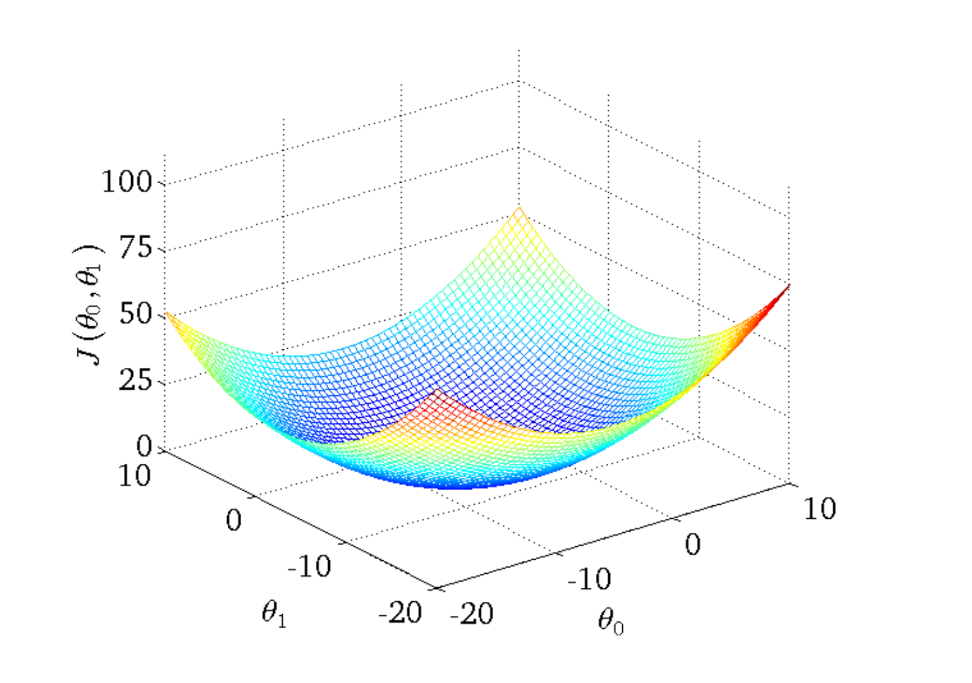
\includegraphics[width=9cm]{img/convex-cost-fn.png}
    \caption{Convex Function Depiction for Cost Function}
    \label{fig:cost-linear-regression}
\end{figure}

\section{Searching for Maxima/Minima}

For non-convex functions, we can have several local minimas and local maximas. Hence, we need a search procedure that can help us "climb up" or "climb down" a hill. Popular methods to do this include Gradient Descent and ADA

\begin{figure}[h]
    \centering
    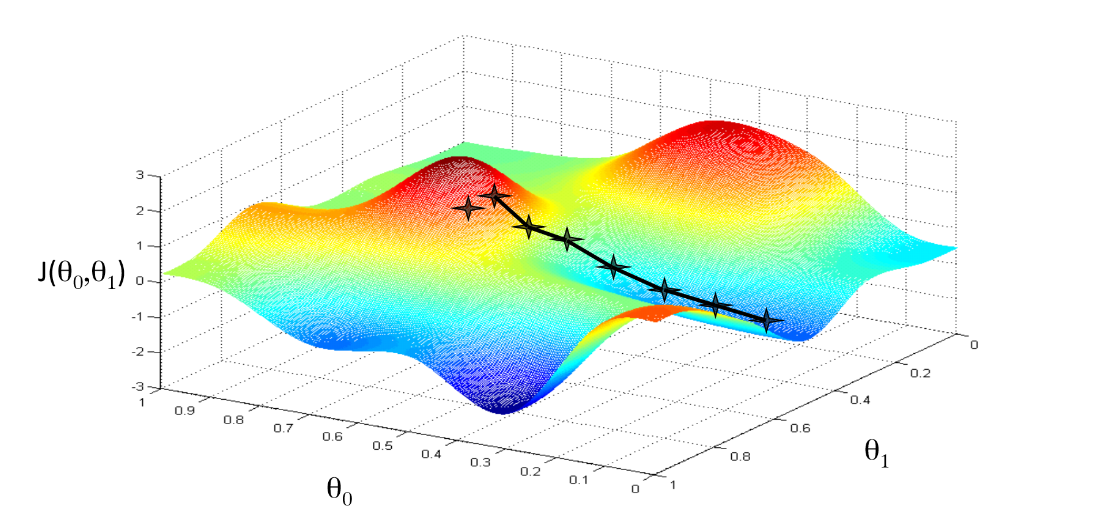
\includegraphics[width=9cm]{img/search-space.png}
    \caption{Search Space Example}
    \label{fig:search-space-example}
\end{figure}

\subsection{Gradient Descent}

The update function for gradient descent is:

\begin{equation}
    \theta_j = \theta_j - \alpha \frac{\partial}{\partial\theta_j} J(\theta)
\end{equation}

This update is done simultaneously to all parameters ($d$ of them). $\alpha$ refers to how quick/large our learning rate is. Essentially, we are moving at an $\alpha$ rate along the function. Larger the $\alpha$, the greater is the step taken.

\subsection{Cost Function Using Taylor Series}

We know that the cost function $J$ for weights $w$ can be defined as $J(w)$. Now, these weights weren't randomly created but rather the result of previous iterations. Or, 

\begin{equation*}
    w^{k+1} = w^k - \alpha\frac{\partial}{\partial w}J(w^k)
\end{equation*}

Now, for vectors, the partial derivative would infact be the gradient. Rewriting, we can say:

\begin{equation}
     w^{k+1} - w^k = -\alpha \nabla J(w^k)
\label{wk}
\end{equation}

Coming to the cost function once again, the cost function $J(w^{k+1})$ can be written as:

\begin{equation}
\begin{split}
    J(w^{k+1}) = J(w^k) + [w^{k+1} - w^k]^T\cdot \nabla J(w^k) + \frac{1}{2}[w^{k+1} - w^k]^T\nabla^2[w^{k+1} - w^k] + \cdots
\end{split}
\label{cost-fn-2}
\end{equation}

Here, we have used the Taylor series to write the cost function. To represent this purely in the form of its derivatives, we must rewrite $[w^{k+1} - w^k]$ in the form of equation \ref{wk}:

\begin{equation}
\begin{split}
    J(w^{k+1}) = J(w^k) + -\alpha \nabla J^T\cdot \nabla J(w^k) + \frac{1}{2}-\alpha \nabla J(w^k)^T\nabla^2J(-\alpha \nabla J(w^k)) + \cdots
\end{split}
\label{jcost}
\end{equation}

\subsection{Ideal Learning Rate}

We can set $\alpha$ depending on the iteration or the point it is at. There is a formula to choose the optimal value of $\alpha$ that uses the hessian. In general, we do not use the hessian since it is computationally intensive and fixing a small value of $\alpha$ will suffice. 

\begin{equation}
    \alpha = \frac{\norm{\nabla J}^2}{\nabla J(w^k)^TH[J]\nabla J(w^k)}
\end{equation}

The above equation can be derived as follows:

If we assume a second order approximation for cost function, we can represent the cost function as follows:

\begin{equation}
\begin{split}
    J(w^{k+1}) = J(w^k) - \alpha\nabla J^T\nabla J(w^k) + \alpha^2 \frac{1}{2} \nabla J(w^k)^TH[J]\nabla J(w^k)
\end{split}
\end{equation}

where $H[J]$ is the Hessian of the cost function (easier to use this notation). Now, to calculate optimum learning rate $\alpha$, we can consider the above equation to be a function of $\alpha$. On taking the derivative of the equation and equating to zero, we should be able to find the optimal value of $\alpha$!

\begin{equation*}
\begin{split}
    &\frac{\partial}{\partial \alpha}J(w^{k+1}) = 0 \\
    &\implies \frac{\partial}{\partial \alpha} (J(w^k) - \alpha\nabla J^T\nabla J(w^k) + \alpha^2 \frac{1}{2} \nabla J(w^k)^TH[J]\nabla J(w^k)) = 0 \\
    &\implies -\norm{\nabla J}^2 + \alpha \nabla J(w^k)^TH[J]\nabla J(w^k) = 0 \\
    &\implies \alpha = \frac{\norm{\nabla J}^2}{\nabla J(w^k)^TH[J]\nabla J(w^k)}
\end{split}
\end{equation*}


Unvectorized calculations of how the partial derivative is taken and calculated can be seen in slide 23 \href{https://github.com/RoboticsIIITH/summer-sessions-2020/blob/master/lecture-slides/deep_learning/linear_regression.pdf}{here}.

We repeat this update function \textbf{until convergence}. This essentially means - stop when the value tends to not vary much. In general, a popular converge is the L2 norm:

\begin{equation}
    \norm{\theta_{new} - \theta_{old}} < \epsilon
\end{equation}

We will notice that slowly and steadily, the global minima will be reached and the value of cost function will reduce, though at a slower rate as iteration count increases.

Coming back to the $\alpha$ value, if we set something too small, it will not converge soon (very slow), but if it is very large, we can actually \textit{diverge}. It may overshoot the minimum and even fail to converge. To see if gradient descent is working, print $J(\theta)$ at the end of each iteration. 

\section{Extending Linear Regression to More Complex Models}

We can modify the input $x$ to not use distinct inputs, but rather powers of a variable - to get higher order fits. Additionally, if have multiple variables, we can even model interactions between these such as $x_3 = x_1\cdot x_2$. Hence, linear regression techniques can be used to fit non linear functions as well.

Generally, 

\begin{equation}
    h_{\theta}(x) = \Sigma_{j=0}^{d} \theta_j \phi_j (x)
\end{equation}

Typically, $\phi_j(x)=x_j$ is the linear basis function. For a polynomial basis function,

\begin{equation}
    \phi_j(x) = x^j
\end{equation}

For a Gaussian basis functions,
\begin{equation}
    \phi_j(x) = exp\Big\{ -\frac{(x-\mu_j)^2}{2s^2} \Big\}
\end{equation}

The sigmoid basis function is:

\begin{equation}
    \phi_j (x) = \sigma\Big(\frac{x - \mu_j}{s}\Big) \text{ where $\sigma$ is the sigmoid function}
\end{equation}

\section{Vectorization}

There are multiple reasons to vectorize - they compress our equations and result in faster code since the operations can be parallelized. Hence, with CPU
s and GPU's the model can be trained faster.

For our model here,

\begin{equation}
    \theta = \begin{bmatrix}
    \theta_0 \\
    \theta_1 \\
    \vdots \\
    \theta_d
    \end{bmatrix} \text{ and } x^T = \begin{bmatrix}
    1 & x_1 & \cdots & x_d
    \end{bmatrix}
\end{equation}

Hence, $h(x) = \theta^Tx$. If we have n such instances, $h(x^{(i}) = \Sigma_{j=0}^{d} \theta_j x_j^{(i)}$, then we can vectorize it as follows:

\begin{equation}
    \theta = \begin{bmatrix}
    \theta_0 \\
    \theta_1 \\
    \vdots \\
    \theta_d \\
    \end{bmatrix} X = \begin{bmatrix}
    1 & x_1^{(1)} & \cdots & x_d^{(1)} \\
    \vdots & \vdots & \ddots & \vdots \\
    1 & x_1^{(i)} & \cdots & x_d^{(i)} \\
    \vdots & \vdots & \ddots & \vdots \\
    1 & x_1^{(n)} & \cdots & x_d^{(n)} \\
    \end{bmatrix}
\end{equation}

The dimensions of $\theta \text{ are } (d+1) \times 1$ and that of $X \text{ are } n \times (d+1)$. Hence, the model in vectorized form are $h_{\theta}(x) = X\theta$. With vectors, the cost function becomes: 

\begin{equation}
    J(\theta) = \frac{1}{2n} (X\theta - y)^T(X\theta -y)
\end{equation}

\section{Closed Form Solution}

Instead of using gradient descent, we can solve for optimal $\theta$ analytically by finding the value that yields $\frac{\partial}{\partial\theta}J(\theta) = 0$. Since this is a convex function, for linear regression, there is just one global minima. The solution is:

\begin{equation}
    \theta = (X^T X)^{-1} X^T y
\end{equation}

We can prove this as follows (L2 norm has been assumed here but it makes no difference really):

\begin{equation*}
\begin{split}
    J(\theta) &= \frac{1}{2n} \sqrt{(X\theta - y)^T(X\theta -y)} \\
    &= \frac{1}{2n} \sqrt{((X\theta)^T - y^T)(X\theta-y)} \\
    &= \frac{1}{2n} \sqrt{(X\theta)^TX\theta - (X\theta)^Ty - y^TX\theta + y^Ty} \\
    &= \frac{1}{2n} \sqrt{(X\theta)^TX\theta - 2(X\theta)^Ty + y^Ty} \\
\end{split}
\end{equation*}

Now, we want to minimize the cost function which implies setting the derivative to 0 and finding the point at which this happens. We will ignore the constant $\frac{1}{2n}$ for ease. 

\begin{equation*}
\begin{split}
    \frac{\partial J}{\partial \theta} &= \frac{\partial \sqrt{(X\theta)^TX\theta - 2(X\theta)^Ty + y^Ty}}{\partial \theta} \\
    &= \frac{1}{2\sqrt{(X\theta)^TX\theta - 2(X\theta)^Ty + y^Ty}} \frac{\partial ((X\theta)^TX\theta - 2(X\theta)^Ty + y^Ty)}{\partial \theta} \\
    &= \frac{1}{2\sqrt{(X\theta)^TX\theta - 2(X\theta)^Ty + y^Ty}} (\frac{\partial(\theta^TXX\theta)}{\partial \theta} - \frac{\partial(2\theta^TXy)}{\partial \theta}) \\
    &= \frac{1}{2\sqrt{(X\theta)^TX\theta - 2(X\theta)^Ty + y^Ty}} (2X^TX\theta - 2X^Ty) \\
\end{split}
\end{equation*}

We reach the final step because of the result obtained in subproblem (a) for the first term, and because the derivative of a matrix multiplication swaps the elements in the second term.

We have to set this to zero, which is equivalent to setting the numerator to 0. Hence,

\begin{equation*}
\begin{split}
    &2X^TX\theta - 2X^Ty) = 0 \\
    &\implies 2X^TX\theta = 2X^Ty \\
    &\implies \theta = (X^TX)^{-1}X^Ty
\end{split}
\end{equation*}

This solution is very slow if n is very large as the order is $n^3$ and gradient descent can work much better for a good $\alpha$ even when $n$ is large.

\section{Regularization}

Regularization is a method to prevent overfitting. This involves adding a term to the cost function that penalizes overfitting using a constant $\lambda$. More on this later. 

\textbf{Interesting Problem:} Find the closed form solution for linear regression, when we have a regularization constant $\lambda$.

A linear regression generally fails to perform classification problems well.

\section{Logistic Regression}

This regression is capable of classifying objects. Let us assume that we have just two classes - 0 and 1. Depending on the value of our hypothesis function (lies between 0 and 1), the class is the value of the function $h_{\theta}(x)$ rounded off to 0 or 1. Generally, we do not just round it off, we set various cutoffs and the output of the hypothesis function can be seen as the confidence of assigning it to a class. 

With a logistic regression model, we want \[ 0 \leq h_{\theta}(x) \leq 1 \]

\begin{equation}
    h_{\theta} = g(\theta^T x)
\end{equation}

\begin{equation}
    g(z) = \frac{1}{1 + e^{-z}}
\end{equation}

Here $g$ is the sigmoid function that only outputs in the range 0-1. You can read up about this online.

Generally, the hypothesis output is the estimates probability of classifying in a particular class on input x. Hence, if $h_{\theta}(x)=0.7$, we have a 70\% change of tumour being malignant.  

When we are trying to separate two given sets, we essentially want a decision boundary to split the data.

\subsection{Cost Function}

We cannot use the cost function from linear regression since it is non-convex for the hypothesis of logistic regression. Refer to \href{https://github.com/RoboticsIIITH/summer-sessions-2020/blob/master/lecture-slides/deep_learning/logistic-regression.pdf}{these slides} for more informatino about the cost function of logistic regression. 

\begin{equation}
\begin{split}
    J(\theta) &= -\frac{1}{m} [\Sigma_{i=1}^{m} y^{(i)}\log h_{\theta}(x^{(i)}) + (1 - y^{(i)})\log (1-h_{\theta}(x^{(i)}))]
\end{split}
\end{equation}

We are required to minimize this function and choose the parameters $\theta$ that accomplish this. We can solve this using gradient descent as well - just by using this cost function.

\subsection{One-vs-All}

This essentially splits a multi-class classification problem into layers of binary classification problems. If we have $N$ distinct classes, then we need $N$ distinct binary classifiers, each designed to recognize just a specific class.2.3-

\chapter{Loss, SVM, Regularization, and Optimization Algorithms}

In a linear classifier, we have an input and a set of weights, and an output that gives some information about what class the object is in. Based on an example in the \href{http://cs231n.stanford.edu/slides/2017/cs231n_2017_lecture3.pdf}{cs231n course}, we can imagine a linear classifier that outputs class scores for every possible class. Hence, a larger number for a certain class means that it is more likely to belong to that class. Ideally, we want the value to be highest in the correct class alone.

\section{Loss Function}

We need a loss function that can help us achieve the above by expressing unhappiness with the scores across the training data. A loss function tells how good our current classifier is given a dataset of examples. The loss over the dataset is the sum of loss over examples.

\begin{equation}
    L = \frac{1}{N} \Sigma \;  L_i (f(x_i, W), y_i)
\end{equation}

Here $i$ examples, $x$ is the input features, $W$ the weights, and $y$ the ideal output while $f$ is the function we prepare. Naturally, loss should be low for correct classification and high for incorrect predictions.

\section{Support Vector Machines (SVM)}

\textit{This portion was not covered in class but is necessary to understand SVM loss - which was covered}

Stealing the following from \href{https://scikit-learn.org/stable/modules/svm.html}{scikit}:

"Support vector machines (SVMs) are a set of supervised learning methods used for classification, regression and outliers detection."

They are useful because they are effective in high dimensional spaces and effective when the number of dimensions is higher than the number of samples. It is a good method to classify with limited amount of data. 

The logic that makes SVM's work is quite interesting. It uses nonlinear data and maps the space to a higher dimension in which a linear solution exists. For instance, if our decision boundary was supposed to be a circle, we define the radius of the circle as a new dimensino $x^2 + y^2$ and can use this to classify circles of varius radii. These transformations are called \textbf{kernels}. \href{https://towardsdatascience.com/support-vector-machine-introduction-to-machine-learning-algorithms-934a444fca47}{This} has some text on what an SVM is. 

\subsection{Margins}

SVM's sound scary but as \href{https://towardsdatascience.com/support-vector-machine-simply-explained-fee28eba5496}{one person put it}, "it becomes less scary once I started to think of support vector machine as a “road machine”, which separates the left,right-side cars, buildings, pedestrians and makes the widest lane as possible. And those cars, buildings, really close to the street is the support vectors." SVM's not only want to find a decision boundary but want to maximize the margin.

Margins are the perpendicular distances between the boundary and the points close to it. Generally, we say that there is a hyper plane that classifies our data as data may not be 2 dimensional and could be of higher dimensions. In SVM's, we let the margin be $[-1, 1]$ or the classes that are formed must have been formed when the hypothesis function yielded values greater than 0 implies $y=1$ and less than 0 implies $y=-1$. Generally,

\begin{equation}
    y\cdot (\beta_0 + \beta_1 \cdot x +  \cdots + \beta_n \cdot x_n) > 0
\end{equation}

As per the previous link once again, "In the linearly separable case, SVM is trying to find the hyperplane that maximizes the margin, with the condition that both classes are classified correctly. But in reality, datasets are probably never linearly separable, so the condition of 100\% correctly classified by a hyperplane will never be met."

\subsection{Kernel Trick}

The following text is \href{https://towardsdatascience.com/support-vector-machine-simply-explained-fee28eba5496}{from the same blog above}.

"What Kernel Trick does is it utilizes existing features, applies some transformations, and creates new features. Those new features are the key for SVM to find the nonlinear decision boundary."

"Think of the polynomial kernel as a transformer/processor to generate new features by applying the polynomial combination of all the existing features."

There are various tricks and transformations that can be used to generate new features. These include polynomial kernels, radius basis kernels (uses distance between all dots to a specific dots).

Andrew NG also seems to have \href{http://cs229.stanford.edu/notes/cs229-notes3.pdf}{detailed notes on this}, but I did not read it.

\subsection{Loss}

This concept was taught with slides from \href{http://cs231n.stanford.edu/slides/2020/lecture_3.pdf}{cs231n}. 

Given an example $(x_i, y_i)$ where $x_i$ is the image and $y_i$ is the integer label.Let $f(x_i, W) = s$, the multiclass SVM loss has the form:

\begin{equation}
    l_i = \Sigma_{j \neq y_i} max(0, s_j - s_{y_i} + 1)
\end{equation}

Here $s_j$ is the score for the class j and $s_{y_i}$ is the real class of the example. This is similar to RELU which is an activation function. We will look at this later. It is generally of the form $f(x) = max(0, x)$. This is also called hinge loss.

\textbf{Interesting Problem: Look at question 7 of the slides}

\section{Regularization}

Imagine that we have a set of points, and we want to create a function to model this data. Now, we can have a very simple function that approximates the points, or a very high dimension one that fits all of training data. The latter cause will usually result in overfitting and may perform poorly for the test data. 

Regularization can be done in many ways but the common way to do it involves adding a term to Loss:

\begin{equation}
    L = \frac{1}{N} \Sigma \;  L_i (f(x_i, W), y_i) + \lambda R(W)
\end{equation}

There are various forms of regularization:

\begin{itemize}
    \item L2: We assume that the weights are a matrix and we sum the squares of all the elements. This likes to "spread out" the weights.
    \item L1: We sum the absolute values of the matrix. This makes the weight matrix sparse - only few non-zero weights.
    \item Elastic Net: It is like the sum of L2 and L1 regularization with a parameter for L2.
    \item More complex: Dropout and Batch normalization. Will be covered later.
\end{itemize}

Regularization helps make the model simpler - occam's razor. 

\subsection{Batch Normalization}

\begin{equation}
    \hat{x} = \frac{x-E[x]}{\sqrt{Var[x]}}
\end{equation}

This forces a gaussian distribution for the inputs-- at the end of every fully connected layers. We can also normalize with mini batch mean and variance. So this would ensure that we don't have a predictable gaussian input. The unit gaussian isn't always the best though because sometimes we want some saturation and choosing a normalization that allows for this gives the network room to learn what's required. 

\subsection{Dropout}

Let's assume that we have a network which can classify well - with it's set of neurons. Some neurons can be imagined to look for certain features (a nose, a tail, etc). With dropout, we remove some of these neurons (squash them to zero) and try getting the model to perform well with this set of neurons. A different subset of units is randomly selected every time we present a training example. Hence, we are able to prevent co-adaptation (presence of all features). The absence of certain features should let us generalize well. This helps prevent overfitting basically.

Look at random forest - start out with a large set of neurons and prune the set as some become unnecessary.

\subsection{Data Augmentation}

This involves modifying existing some images in certain ways - change the orientation, dimensions, or "augment" it. We then train the data on this. We can have a random set of crops/scales as well, shear, and much more.

\subsection{DropConnect}

In drop connect, we drop certain connections (set some weights to zero) instead of the nodes, so they can remain partially active. DropConnect is a generalization of DropOut because it produces even more possible models, since there are almost always more connections than units. However, you can get similar outcomes on an individual trial. 

\subsection{Mixup}

In mixup, we train on random blends of images (blend the pixels of various images for instance). This has been found to improve generalization. Google for more details.

\subsection{Transfer Learning}

We always need a lot of data to train a neural network. We can do this without data augmentation using "Transfer Learning". As the name suggests, you ‘transfer’ the weights the network learns and learn some more with the small dataset. That is, you fine tune the network for the new dataset, keeping the weights of the previous one. The myth that we need a large dataset is hence broken for training networks. This makes sense for similar data as a result where fine tuning is more benefitial than training from scratch. This is called 'restore model' since we are restoring the state from a previously trained network and continuing from there. 

\section{Softmax Classifier (Multinomial Logistic Regression)}

Let us assume that we have a vector $s$ of real numbers. The softmax function will take this vector as an input and assign probability scores to each of the element as follows:

\begin{equation}
    \sigma(s)_k = \frac{e^{s_k}}{\sum_j e^{s_j}}
\end{equation}

Now when applied, this will give us a column vector with probabilities for each class. Now, to get the loss for the example $i$ is:

\begin{equation}
    L_i = -\log P(Y=y_i | X=x_i) \text{where $y_i$ is the correct classification}
\end{equation}

Clearly Softmax function is extremely useful for classification problems. One question that may come up is "Why use softmax instead of normalizing the values derived?". As per \href{http://93.174.95.29/main/11874B3F9B89BAB4C7826272B2EFC032}{section 2.3.3 of Deep Learning by the "godfathers of AI"}, having exponentiated variables help since we tend to calculate the log likelihood.

This is also called cross-entropy loss. Since, this error is given as a probability, it's easier to visualize the error with Softmax. Unlike SVM, where we cannot infer any such thing.

\section{Stochastic Gradient Descent}

Gradient descent is computationally inefficient when the dataset is very large as for every update step, we need to calculate average loss across all examples. Additionally, the drop in loss may not be much to begin with. Hence, we can use "minibatches" as sample of the training data for gradient descent. This sample can be arbitrary and not fixed. Hence, this will perform better. In online stochastic gradient descent, size of minibatch is 1.

The problem with stochastic gradient descent is that it is more sensitive to only certain weights. Hence, it's making very slow progress to reach the global minima as the progress along a certain dimension due to a lack of sensitivity in one dimension. This is possible since we are using mini-batches and noise may easily get into our data.

Problems also exist with local minima and with flat surfaces as the global minima cannot be reached. 

\section{Other Optimization Methods}

Gradient descent was an algorithm that helped us explore our search space. It is also called an optimzation algorithm. They essentially serve the purpose of minimizing our loss function. Gradient descent isn't the only such method! Few more optimization methods are discussed in the 'Optimization' chapter in the SLAM section. While the ones in this section may focus on variations of SGD, they tend to focus on second order approximations (kinda). The concepts are one and the same - getting a quicker, better convergence.

\subsection{SGD + Momentum}

This is something that will commonly be used. In a regular SGD, we use the regular update equation as stochastic gradient descent. In SGD+Momentum, we also calculate velocity and rather than moving in the direction of negative gradient, we move in direction of velocity. The idea is that even at a local minima, the "ball" stuck at the local minima will have momentum and velocity. Now, if we have a local minima it will likely be a small hill and using this momentum we can escape the local minima. Even at saddle points (flatish surfaces), there is some velocity as well and hence we can move from this position. 

We don't just go in direction of velocity but with the weighted sum of velocity and gradient.

If SGD was \[ x_{t+1} = x_t - \alpha \nabla f(x_t) \]

Now, in SGD + Momentum:

\begin{equation}
\begin{split}
    v_{t+1} = \rho v_t - \alpha \nabla f(x_t) \\
    x_{t+1} = x_t + v_{t+1}
\end{split}
\end{equation}

From cs231n notes:

As an unfortunate misnomer, this variable $\rho$ is in optimization referred to as momentum (its typical value is about 0.9), but its physical meaning is more consistent with the coefficient of friction. Effectively, this variable damps the velocity and reduces the kinetic energy of the system, or otherwise the particle would never come to a stop at the bottom of a hill. 

\subsection{AdaGrad}

AdaGrad keeps a runnning sum estimate of the squared gradients. So instead of velocity, we have a "gradient squared" term. The update equation is essentially:

\begin{equation}
\begin{split}
    x_{t+1} = x_t - \alpha \frac{\nabla f(x_t)}{\sum_t (\nabla f(x_t))^T + 1e^{-7}} \text{ where 1e-7 is to prevent 0 division }
\end{split}
\end{equation}

\textbf{Why does this help?}

If our gradient is high, then the square of the gradient will be higher. If gradient is low, then dividing by this makes the update more sensitive to a lower sensitvity variable. In AdaGrad, progress along ‘steep’ directions is damped and progress along ‘flat’ directions is accelerated. But over time, the step size gets smaller and smaller. It’s good in the convex case because as you approach the minima, you want to slow down and converge. But in non convex case, if you come across a saddle point, you get stuck and can’t make any progress.

\subsection{RMSProp}

The problem with AdaGrad is that the sum of gradient squares will become very big constantly. And, in the end we'll be taking very tiny steps towards minima. RMSProp solves this. It is a leaky AdaGrad. Here, we'll just let the sum of gradient squares \textbf{decay} over time as can be seen in figure \ref{fig:rms+prop}.

\begin{figure}[h]
    \centering
    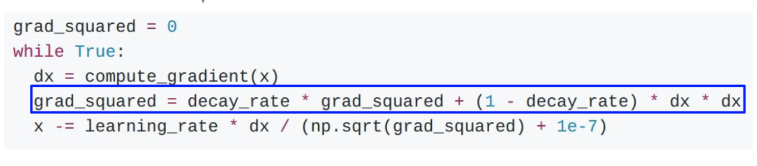
\includegraphics[width=12cm]{img/RMSProp.png}
    \caption{RMS Prop Calculation}
    \label{fig:rms+prop}
\end{figure}
\subsection{Adam}

The core idea behind momentum is to move in the direction of velocity to not get stuck in a local minima. The core idea behind AdaGrad was to compute the square of the gradients to slow down movement along the sensitive direction and prevent zig-zags. The core idea behind Adam is to combine the two! This can be seen in \ref{fig:adam}.

\begin{figure}[h]
    \centering
    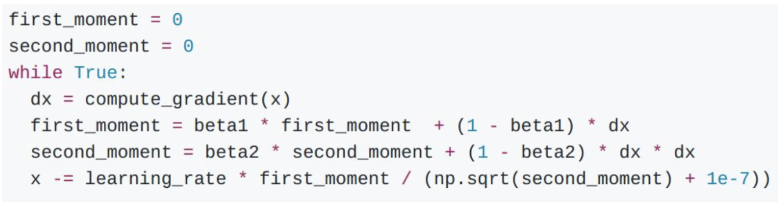
\includegraphics[width=12cm]{img/adam.png}
    \caption{Adam Calculation}
    \label{fig:adam}
\end{figure}

The problem with Adam is that at the first step the second moment is 0. Hence, when divided by such a small near 0 quantity, the value of $x$ will change significantly. This is a problem with RMSProp/AdaGrad as well. Of course, since the first moment is also very small, it may cancel out the second moment, but sometimes, it does result in taking very large steps in the beginning. This is solved with a bias correction step.

\href{https://youtu.be/_JB0AO7QxSA?t=2588}{cs231n} covers these quite well.

Adam is the best algorithm and converges really quick. Abhinav vouches for it. His recommendations for setting up Adam are:

\begin{enumerate}
    \item beta1 = 0.9
    \item beta2 = 0.999
    \item learning\_rate = 1e-3 or 5e-4
\end{enumerate}

\subsection{Misc: Learning Rate $\alpha$}

It is the number by which we multiply the resulting gradient by. The size of the steps that we take across iterations are defined by learning rate. Generally, as the loss value reduces, we lower the learning rate - slow down as we are nearly about to converge. SGD, SGD+Momentum, AdaGrad, RMSProp, and Adam all have learning rate as a hyperparameter.

‘Step Decay’ - we reduce the learning rate at particular steps, so if it would’ve gotten stuck somewhere, we can take smaller baby steps and maybe reach a better region. 

\section{Data Processing}

Before training the model, it is important that our input data meets certain standards and model isn't regularized. We've already seen how regularization helps generalize the model. Another way of ensuring this is to modify the input data with data preprocessing.

We can imagine that the input data has high variance and is off center (not near origin). Hence, we can zero-center the data - subtract mean of data from each element of the dataset. We can then divide the dataset by the standard deviation of the datasetand normalize the dataset. This helps prevent gradient extinguishing and gradient explosions. 

\chapter{Neural Networks and Backpropogation}

When dealing with increasingly complex data, it is not practical to deal with linear score functions with just a single weight matrix. These are usually of the form $f = Wx$. With a neural network, we can have a non-linear function that let's us obtain more complex decision boundaries.

3Blue1Brown videos are a great source to learn about Neural Networks. They are now the state of the art for machine learning and widely used for a variety of applications. From images to language processing, variations of neural networks are common. 

Neural networks are very powerful and perform a wide variety of tasks. They are universal function approximators. Now, contrasting with our previous linear function, we can imagine that a 2-layer Neural Network $f=W_2 max(0, W_1 x)$. Here $x \epsilon R^D$, $W_1 \epsilon R^{H\times D}$, $W_2 \epsilon R^{C \times H}$.

Similarly, for a 3-layer neural network, $f=W_3max(0, W_2max(0, W_1x))$. Visualizations of this can be seen in \href{http://cs231n.stanford.edu/slides/2020/lecture_4.pdf}{cs231n} slides.

\section{The Probability Explanation}

Neural networks essentially model the maximum likelihood estimate. Look at it this way: We have a set of parameters, that with our input give us an output. We want the output to be the best possible one (so for a classification problem, increase the probability of the correct class). Training a neural network does that! The best set of parameters is subsequently the maximum likelihood estimate. 

Why do we use negative log likelihood? Well, both are the same. Truly. They represent the same probabilistic distribution and the best values are the same. It's just that we negative log likehood because we want to minimize the loss function.

\section{Activation Functions}

There are various activation functions which are all non-linear. The previous equations used $max$ which is a non linear function. This is an example of an activation function ReLU. RELU is the most common activation function and widely used. Leaky-RELU is also used. The cs231n slides has a great list of possible activation functions. We don't tend to use sigmoid since it tends to kill gradients. Gradients will vanish and hence, can't be used for neural networks. It's the same thing for $tanh$.

\textit{For more on vanishing gradients in sigmoids and dying ReLUs, look at \href{https://medium.com/@karpathy/yes-you-should-understand-backprop-e2f06eab496b}{these notes by Andrej Karpathy}.}

This is also covered in some more depth in the "Training" section of the chapter.

\section{Architecture}

\begin{figure}[h]
    \centering
    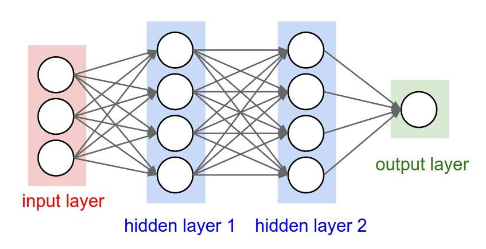
\includegraphics{img/Neural Network.png}
    \caption{Neural Network}
    \label{fig:neural-network}
\end{figure}

The neural network can be visualized to have an input layer - for its features, hidden layers (determined by the matrices in between), and an output layer. For a regression problem, the output layer would just be a single node but for a classification problem it would likely be the number of classes.

The "forward pass" refers to calculation process, values of the output layers from the inputs data. It's traversing through all neurons from first to last layer.

The loss function is calculated from the output values. 

And then "backward pass" refers to process of counting changes in weights (de facto learning), using gradient descent algorithm (or similar). Computation is made from last layer, backward to the first layer.

\textbf{Sidenote:} There is a problem with ReLU - dead neurons since gradient is 0 since ReLU is 0 when input is less than 0. Hence, leaky ReLU was created. However, ReLU has been found to be better in some instances.

There is only one cost function for a neural network - one for the entire network - not for each layer.

\section{Backpropogation}

In gradient descent, we calculated derivative/gradient and used that information to change our input. This was a gradual change and essentially decided by the change of the function with respect to the parameters. The same can be thought of for neural networks. The weights of each layer will determine the effectiveness of the network and hence, we need to set these weights appropriately. Unfortunately, it is not easy to calculate gradient manually. This is where the idea of backpropogation comes into the picture. 

"Backpropagation is for calculating the gradients efficiently, while optimizers is for training the neural network, using the gradients computed with backpropagation. In short, all backpropagation does for us is compute the gradients. Nothing more." from \href{https://mlfromscratch.com/neural-networks-explained/#/}{this.}

To understand the way this works pictorially, look at computation graphs in the \href{http://cs231n.stanford.edu/slides/2020/lecture_4.pdf}{cs231n slides}.

\href{http://neuralnetworksanddeeplearning.com/chap2.html}{This} is a very detailed source to understand backprogation. It is from a larger book about neural networks.

The way we might discover how to calculate gradients in the backpropagation algorithm is by thinking of this question:

\textit{How might we measure the change in the cost function in relation to a specific weight, bias or activation?}

\subsection{Intuition}

The 3Blue1Brown video explains backpropogation really well. Let us assume that we have just one example, and a neural network with a few hidden layers. Based on the weights and biases at these layers, we get an output vector with varying degrees of "activation". Now, each of these nodes will also have an ideal activation. For instance, our neural network may assign a score of 0.2 to a node, when ideally it is 1. How did we get this score? This score is the sum of the product of weights and the activation of the previous layer. So, we want to increase the activation of certain nodes in the previous layer and try increasing their importance as well - as long as they can help increase our output score. Vice versa, if our output score is higher than required, we want to reduce the values of weights and activation in previous layer. We can also bring about a change in the output by changing the bias. Note how we have identified the importance of the bias, and weights in some form. We see that there is a requirement to proportionally increase/decrease weights. This is just in regard to a single output node! Each output node will have connections to the previous layer and will also have some "requirements" about how much the weights should be tweaked. The idea is - if we satisfy the request of all these nodes, we are closer to a perfect solution. But is this the end? No.

The previous layer has now received some requests about how it should change. There may be other hidden layers though. Hence, we must recurse and move \textbf{backwards} through the network.

This was just for one training example! If we follow this routine and see what changes each example desires, and average it - it is essentially the negative gradient of the cost function.

\subsection{Simplified Math}

\href{https://www.youtube.com/watch?v=tIeHLnjs5U8}{A video by 3Blue1Brown} - obviously. Is very useful to understand what the gradients we are calculating represent. As mentioned earlier, calculating gradients manually is a pain.

In backpropogation, we measure the partial derivative of the cost function to weights, biases, and even the activation of previous layers.

Let us assume that we have a function such as $q = x + y$. This output $q$ is then fed to another function $f$ which is the final output of our computation graph. For ease refer to this example in figure \ref{fig:c_graph}.

\begin{figure}[t]
    \centering
    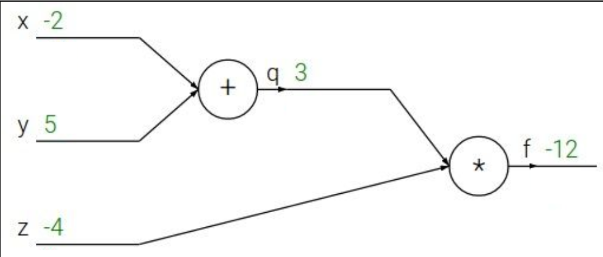
\includegraphics{img/computational-graph.png}
    \caption[width=5cm]{Computation Graph for Backprop Example}
    \label{fig:c_graph}
\end{figure}

Now, if we try to calculate the partial derivative of $f$ with respect to input $y$, we cannot directly compute it. We must use chain rule such that we get \[ \frac{\partial f}{\partial y} = \frac{\partial f}{\partial q} \frac{\partial q}{\partial y} \]
Here we refer to $\frac{\partial f}{\partial q}$ as the upstream gradient as it is a gradient that is not local to $y$ in some sense. The local gradient here is $\frac{\partial q}{\partial y}$. The product of these two may then be relevant as an upstream gradient for another partial derivative (assume that $y$ was also a function). Hence, with respect to this particular function, this is the downstream gradient.

\subsubsection{Patterns in gradient flow}
We observe that the addition operation is a \textit{gradient distributor}. This is because local gradient is 1.

The multiplication gate is a \textit{swap multiplier}. This is because local gradient is the other variable in the multiplication. Hence, we multiply the other input with the upstream gradient.

This is essentially what happens in backward pass. Obviously, note that the graph must be topologically sorted for us to calculate gradients properly since we constantly need an upstream gradient. Traversing in the reverse order of a topological sort will guarantee this.

\subsection{Real Math}

So far, we've done backpropogation with scalars (in the computational graph). But what about vector valued functions? - the type we'll be dealing with in neural networks.

Let us assume that we have $x \epsilon R^N$, and $y \epsilon R^M$ - they are both vectors. To see how for each element of $x$ changes, how $y$ changes requires vector derivatives - the Jacobian

I would write this part entirely but there is already an amazing resource for this - \href{https://github.com/RoboticsIIITH/summer-sessions-2020/blob/master/lecture-slides/deep_learning/backprop_linear_layer.pdf}{notes by Justin Johnson}. It describes how upstream gradients can be assumed to be give, and we need to calculate the local gradients. When we look at the dimensions, the local gradient is in fact a Jacobian. This matrix is so large that it often cannot even fit in memory! Hence, we are forced to compute the product of local and upstream gradient without explicitly calculating the Jacobian. The PDF describes this very well but in the end, we find that for a function such as $Y=XW$, then for $L$ - the loss function, 

\begin{equation}
    \frac{\partial L}{\partial X} = \frac{\partial L}{\partial Y} W^T
\end{equation}

Similarly, to calculate $\frac{\partial L}{\partial W}$ without the Jacobian $\frac{\partial Y}{\partial W}$ with:

\begin{equation}
    \frac{\partial L}{\partial W} = X^T \frac{\partial L}{\partial Y}
\end{equation}

This strategy of thinking one element at a time can help you to derive equations for backpropogation for a layer even when the inputs and outputs to the layer are tensors of arbitrary shape.

\subsubsection{Backprop for ReLU}

\begin{equation}
    \Big( \frac{\partial L}{\partial x} \Big)_{i} = \begin{cases}
       \Big(\frac{\partial L}{\partial z} \Big)_{i} &\quad\text{if} x_i > 0\\
       \text{0} &\quad\text{otherwise}\\
     \end{cases}
\end{equation}

\subsection{Micrograd}

Micrograd is a tiny autograd engine that let's us easily understand all the previous concepts of gradients. It is meant to understand how gradients are calculated, and how backward propagation works. \href{https://github.com/RoboticsIIITH/summer-sessions-2020/blob/master/lecture-slides/deep_learning/vector_derivatives.pdf}{These slides (at the end)} has some code snippets from the original \href{https://github.com/karpathy/micrograd}{repository}. It is worth looking at to get a rudimentary understanding of how pytorch works.

\section{Training}

The basic pipeline for training a neural network is:

\begin{enumerate}
    \item Sample out a batch of data
    \item Forward propagate it
    \item Compute loss at the end
    \item Propagate and calculate gradients on the way back
    \item Using one of the optimization methods, update the parameters/weights by taking steps in the direction of negative gradient.
\end{enumerate}

We've already seen optimization algorithms earlier. We can use one of them.

\section{Activation Function}

\subsection{Sigmoid}

\begin{equation}
    \sigma(x)=\frac{1}{1+e^{-x}}
\end{equation}

It is problematic because saturated neurons tend to kill gradients. Or, when the inputs are extremely positive or negative, the gradients are zero cause the curve is flat in that region. 

It is not zero centered.

It is also computationally expensive cause of exp() - not a huge concern.

\subsection{tanh}

This is luckily zero centered but can still kill gradients

\subsection{ReLU}

This does not saturate in the positive region, is very fast for computation and for convergence.

But, this is also not zero centered output and gradient is saturated for negative weights. 

If we have bad initialization, then some neurons may never activate and we'll have dead ReLU. It can also die while training. 

\subsection{Leaky ReLU}

\begin{equation}
    f(x) = \max (0.01x, x)
\end{equation}

This solves the problem of dying ReLU.
PreReLU and ELU also solve the same problem.

\subsection{ELU}

ReLU (rectified linear units) is a very popular choice for an activation function. But, in a \href{https://arxiv.org/pdf/1511.07289.pdf}{recent paper}, it was shown that "Exponential Linear Units" (ELU) tend to converge the cost function better.  Like  rectified linear units (ReLUs), leaky ReLUs (LReLUs) and parametrized ReLUs (PRe-LUs), ELUs alleviate the vanishing gradient problem via the identity for positive values. ELUs have a gradient for negative values as well but it converges as the value reaches a certain $\alpha$.

\subsection{Maxout "Neuron"}

\begin{equation}
    \max (w_1^T + b_1, w_2^T + b_2)
\end{equation}

This generalizes ReLU and Leaky ReLU, doesn't saturate or die.
But it doubles the number of parameters.

\section{Data Preprocessing}

This was already mentioned briefly earlier. We can normalize data so that the range of all data is the same. Though, in practice zero-centered data is sufficient for images at least. We also see things such as PCA, whitening as data preprocessing. This isn't applied for images usually though. In practice, AlexNet subtracts the mean image. VGGNet subtracts the mean image along each channel.  

\section{Initialization}

Initialization is a very tricky thing. If we have very small weights, after multiple epochs, the output can become smaller and smaller. Large weights can also make values explode such that it can't even be calculated. This is because when the range of the weights is uncontained, it can "build up" and get better. Ideally, we want to have a standard deviation of around 1 for each weight. \href{https://towardsdatascience.com/weight-initialization-in-neural-networks-a-journey-from-the-basics-to-kaiming-954fb9b47c79}{This} blog article has a decent illustration of how values can explode or die to 0. Little things such as good weight initialization can make the difference between good and bad performance.

\subsection{Xavier Initialization}

The naive method of initializing in a uniform distribution of [-1, 1] and then dividing by root of number of inputs proved to be bad in practice. In fact, it essentially killed gradients as research by \href{http://proceedings.mlr.press/v9/glorot10a/glorot10a.pdf}{Xavier Glorot and Yoshua Bengio shows.} They then proposed Xavier initialization.

"Xavier initialization sets a layer’s weights to values chosen from a random uniform distribution that’s bounded between $\frac{\sqrt{6}}{\sqrt{n_i + n_{i+1}}}$ where $n_i$ is the number of incoming network connections, or “fan-in,” to the layer, and $n_{i+1}$ is the number of outgoing network connections from that layer, also known as the "fan-out.". To drive the point home, Glorot and Bengio demonstrated that networks initialized with Xavier achieved substantially quicker convergence and higher accuracy on the CIFAR-10 image classification task.

"Conceptually, it makes sense that when using activation functions that are symmetric about zero and have outputs inside [-1,1], such as softsign and tanh, we’d want the activation outputs of each layer to have a mean of 0 and a standard deviation around 1, on average. This is precisely what our home-grown method and Xavier both enable."

\subsection{Kaiser Initialization}

"But what if we’re using ReLU activation functions? Would it still make sense to want to scale random initial weight values in the same way?" from \href{https://towardsdatascience.com/weight-initialization-in-neural-networks-a-journey-from-the-basics-to-kaiming-954fb9b47c79}{the same article as before}.

Here, it seems that regular normal distribution can work decently well, when scaled by a constant. Kaiser et al showed that when we scale the weights of the matrix are scaled by the square of $2/number\_of\_input\_nodes$, the standard deviation across weights is just 1! This is very desirable since this ensures that our gradients don't explode or vanish for varying network depths. In fact, it was shown that this initialization performed significantly better than Xavier initialization when using ReLU activation. The error did drop, unlike Xavier.

There's a lot more to initialization but this is some decent intuition on how it isn't a non-issue. As with a lot of hyperparameters and design choices, they are interrelated.

\href{http://karpathy.github.io/2019/04/25/recipe/}{This blog article by Andrej Karpathy} is a good explainer on training neural networks and good practices. Naturally, when there are so many things that one can do in deep learning, there are twice as many things that can go wrong. The blog article describes some good steps such as data exploration, visualization, baseline performance, and more to get started.

\section{Software}

\subsection{CPU vs GPU}

CPUs and GPUs are quite different. GPUs were created for graphic processing reasons. The differences between CPUs and GPUs are large though.

GPUs have a large number of cores and a low clock speed. They aren't great at doing a variety of tasks but can do a lot of tasks simultaneously. 

Convolutions are parallelizable for instance, and can take advantage of GPU.

Nvidia has CUDA - it is a C like code that runs directly on gPU. It has high level APIs like cuBLAS (Matrix multiplication and such). OpenCL is a generalized thing that runs on many GPUs but is not optimized and is quite slow.

\subsection{Frameworks}

When we come to implementing neural networks, we tend to use PyTorch. PyTorch is extremely useful since it automatically calculates gradient for us using \textit{autograd}. The summer session also included tutorials on pytorch but I have not written about it. \href{https://github.com/jcjohnson/pytorch-examples}{Justin Johnson has a really cool} resource that introduces you to PyTorch.

Keras is a high level tensorflow API to get models running - but it feels incorrect to use. Is better to do things from scratch since neural networks aren't really APIable since there are so many things to tweak and monitor.  

Caffe is a c++ deep learning framework with a python interface. Hence, it's faster than usual and is used in production.

To see if our neural network is good, it is a good idea to take a small training set and see if we can overfit to this data - loss 0. Learning rate choice can also greatly impact the performance of the network and may lead to exploding cost. 



\chapter{Convolutional Neural Networks}

CNN's are commonly misunderstood to be used just for images, which is false! They are also used for semantic parsing, search query parsing, sentence prediction and more - language tasks! They are obviously popular because of their uses for images though. CNN's can be used for image recognition, classification, and detection. Recognition and detection are different; it's one thing to identify a person as a human and another to know what specific person it is. These neural networks are also used for videos - not just images. If we are trying to track an individual through space and predict where they will be - CNN's can be used.

For now, let's think of ConvNet (CNN) as a black box to which we feed an input, and get an output. To complicate things, we send the output of ConvNet to a feature map (they describe the image in a certain way), and pass it through FC Layers (normal fully connected layers of a neural network).

\textbf{Note (New Terminology - recap of NN):} A perceptron is a node in our neural network that is decided by the product of weights and activations in the previous layer. The input to a node along with the weights for each determine the activation of a certain perceptron. This is then used to compute the perceptrons for the next layer. A fully connected layer is one in which each perceptron in a layer, is connected to all perceptrons in the previous layer.

\section{Architecture}

\href{https://cs231n.github.io/convolutional-networks/#overview}{These notes} by cs231n cover the general architecture (input -> conv -> relu -> pool -> fully connected -> class scores). Look at this after some general reading about CNNs

\section{Convolutions}

A convolution is a mathematical operation on two functions that produces a third function that expresses how the shape of one is modified by the other. Mathematically,

\begin{equation}
    (f * g)[n] = \Sigma_{m= \infty}^{\infty} \; f[m]g[n-m]
\end{equation}

where $n$ is the timestamp. This is slightly hard to understand immediately but signal processing might help understand. This is like a one-dimensional convolution.

The 2D convolution is fairly simple to understand. If we have a kernel - a small matrix of weights. The kernel "slides" over the 2D input data, performing an element wise multiplication with part of the input it is current on, and summing up the results into a single output pixel. Hence, we get a new 2D matrix from our 2D matrix of features.

To see how this works, look at a gif of how convolution works. It is commonly visualized as a matrix tile that is traversing through a larger matrix.

\subsection{Some Uses}

\begin{figure}[h]
    \centering
    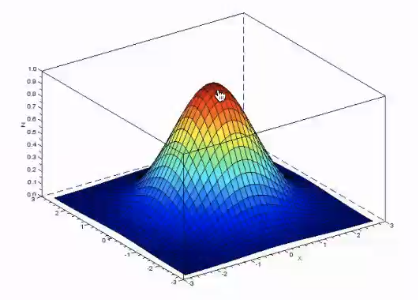
\includegraphics{img/3d-gaussian.png}
    \caption{3D Gaussian}
    \label{fig:my_label}
\end{figure}

Blurring (like blurring an image) can essentially be thought off as taking an average of adjacent pixels. For blurring using convolutional neural networks, we will use an averaging filter that has a gaussian distribution (like the image shown). Here, the central pixel will have the most importance. 

CNN's can also be used for edge detection. For instance, laplacian filter will take a gaussian kernel, and another one, and take the derivative (read more). So these filters help us achieve a lot of things, and convolving a filter with a certain image gives us a response that represents how that portion of the image is represented with respect to our filter.

\section{Techniques}

\subsection{Padding}

Now, if we use a filter and convolute, we get a smaller output matrix. In fact, the corners of the image will never correspond to the center of the filter. This is where padding is generally used. We pad the matrix on the outside with 0's (Zero is usually used) and this lets us get a larger output matrix. Hence, we apply convolutions after padding. The pixels that were previously getting "ignored" because they were at the edge come to focus as they now have neighbouring elements.

\subsection{Striding}

Striding is used to get an output that is smaller than the input.

\subsection{Dilation}

\begin{figure}[hbtp]
    \centering
    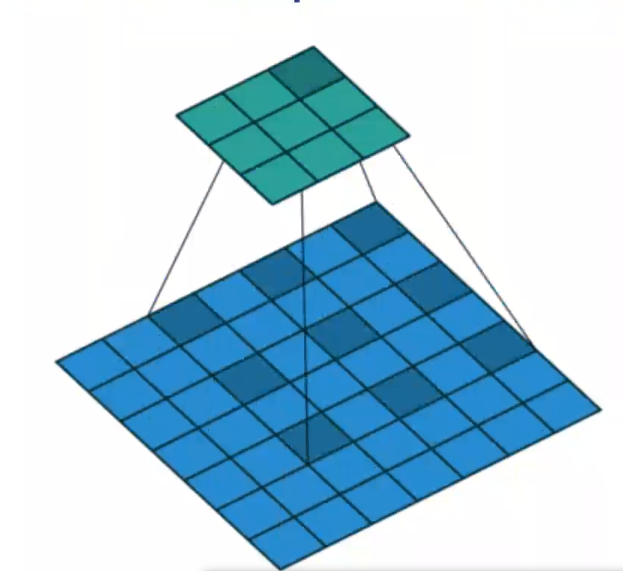
\includegraphics[width=5cm]{img/dilation-cnn.png}
    \caption{Dilation}
    \label{fig:dilation}
\end{figure}

In dilation, we don't choose adjacent elements from our input matrix - but leave gaps in the matrix.

The dimensions of the output matrix on applying the previous techniques would be:

\begin{align}
    H_{out} = \floor{\frac{H_{in} + 2\times \text{padding}[0] - \text{dilation}[0]\times (\text{kernel\_size}[0] - 1) - 1}{stride[0]} + 1}
\end{align}

\begin{align}
    W_{out} = \floor{\frac{W_{in} + 2\times \text{padding}[1] - \text{dilation}[1]\times (\text{kernel\_size}[1] - 1) - 1}{stride[1]} + 1}
\end{align}

In practice, most inputs have 3 channels (RGB). In such scenarios, we apply the kernel over the red, green, and blue channels. It is possible that some filters work best for a particular channel and hence, we can use different kernels/filters for each channel as well. Now, we will get 3 processed versions which can then be summed together to form one channel. Generally, the average is taken. 

We usually also have a bias term that shifts the channel output (every single element in the matrix). 

We can combine the idea previously mentioned by considering our input as a 3-dimensional input, and our filter as a 3d layer as well that convoles with the image. 

Now, if we have different filters, we will get different activation maps. For 10 filters, 10 activation maps (we have to design this). When training a CNN, the learning process involves deciding what these filters should be - what the weights should be. These are the feature maps of the image. We can't decipher what features will be useful by just looking at the images.

VGG-16 is a very popular Convolution Network and when their features are visualized, the low level features were unintuitive - lines and corners, slanting lines, and so on. These filters essentially captured the texture of the image. 
The subsequent features, mid level features, were more intricate than low level and captured more information about the colour and gradients across the image(the way the shade changes). Further, the high level features represented even more subtle nuances of the image. 

\section{Non Linearity Layer}

Generally, ConvNet is a sequence of convolutions and non-linear operations such as ReLU (applied element wise). It's important to have non-linear operations in between otherwise, all layers could be combined into one layer. The non-linear function let's us get more complex decision boundaries. 

Non-linearity doesn't really mean that we lost information but rather that we are able to have to have better boundaries.

What we get after the convolution layers are called convolutions (and can be understood as features in some form). But, it is only after the non-linearity that we are able to get usable features. One doesn't make sense without the other.

\section{Fully Connected Layer}

We can flatten an image (3 Dimensional) into a single vector ($x \times 1$). This can be treated as our input. Then as usual, in a neural network $Wx$, choosing a \textit{$\text{number of new neurons } \times \text{ number of weights}$}.

Flattening the image WILL result in spatial information. This is why we use Convolutions so that we can encode spatial information prior to flattening. They essentially linearize the feature maps that we get.

\section{Pooling Layer}

It makes the representation of the feature maps more manageable and downsamples the image. If we had an image of a big car, if we downsample to a smaller size, we are giving the network opportunity to recognize images of various sizes. This does result in a loss of information but it will also result in result in more economical data.

\section{Steps Summarized}

The steps for a full fledged CNN may be:

\begin{itemize}
    \item Provide Input image to Convolutional Layer
    \item Choose parameters, apply filters with strides, padding if required. Perform convolution on the image and apply ReLU activation to the matrix.
    \item Perform pooling to reduce dimensionality size
    \item Add conv layers as required
    \item Flatten output and feed into a fully connected layer
    \item Output the class using an activation function and classifies image.
\end{itemize}

Look up \href{https://dzone.com/articles/the-9-deep-learning-papers-you-need-to-know-about-1}{these}.

\section{DeConv}

??? Something that can undo convs?

\chapter{Recurrent Neural Network}

So far, we've usually considered networks that are feed forward - we keep moving forward in a network. But sometimes, we want to have variable outputs, variable input (sentiment analysis with varying sentences), or both (machine translation for instance). This is where recurrent neural network comes in. 

In general, RNN have a core cell that takes an input. The RNN has an internal hidden state that gets updated when there is a new input.

\begin{equation}
    h_t = f_W(h_{t-1}, x_t)
\end{equation}

where $h_t$ is the new hidden state, $f_W$ a function with parameters $W$. $x_t$ is the input at time $t$, and $h_{t-1}$ is a hidden state that will get updated with the new input. Note that the parameters don't change with time.

So this function could look like

\begin{align}
    h_t &= tanh(W_{hh}h_{t-1} + W_{xh}x_t) \\
    y_t &= W_{hy}h_t
\end{align}

So the computational graph would have a series of hidden states with function blocks inbetween that take different inputs. The hidden states can then be fed to another layer that gives an output y. This output $y$ could have a loss. Hence, we'll have a loss for each input and we can combine all the loss.

Depending on the situation, we will determine what outputs are relevant. So for sentiment analysis, the final hidden state's output will be desired. 

In many-to-many networks, we can use an encoder-decorder model where we have many-to-one + one-to-many. 

\textbf{MultiLayer RNN}

Here, we have various hidden states for a single layer of the RNN, and so on for every layer. Generally, super deep RNNs aren't very common. 

\section{Training}

RNNs are commonly used for language modelling problems. During a forward pass, it may take letters at various steps. So, for a letter prediction model, we want the output from each hidden state to be ideally the next letter (from our training example). Now, if we train this model with various sequences, we should ideally get a decent predictive network. '

What's interesting here is that we are training a network based on input it receives over time, or we will backpropogate through time. This is bad because we have a lot of inputs often and it is not efficient to do iterative algorithms for large inputs when we make tiny steps. 

Hence, we tend to use truncated backpropogation, where we don't backprop ALLL the way to the start, but do it only for a set of hidden states. Hence, we train group by group. This is analogous to SGD where we use minibatches to train our data. 

Now, we can rewrite the function earlier as follows:

\begin{equation}
    h_t = tanh(W\begin{bmatrix}h_{t-1}\\
    x_t\end{bmatrix}) \text{ where $W$ is $(W_{hh} W_{xh})$}
\end{equation}

Now, note that the gradient of this is the transpose of the weight matrix, imagine that when we compute gradient, we are essentially chaining a lotttt of these matrices. Then, our gradient will explode when we have large time ranges. This is usually solved by clipping gradients. But, gradients also vanish (get too small) which is a harder problem. This is solved by LSTM (explored later)

\section{Image Captioning}

There are various approaches to image captioning but in one approach, we have a CNN that feeds into a hidden state, and the RNN will have various elements of the image as inputs. Then, we can run this in a supervised nature with text captions. 

\section{LSTM}

LSTMs are long short term memory and were introduced long ago (1997 or so). In a vanilla RNN, we have a hidden state, but in LSTM we have two hidden states $c_t$ and $h_t$, where $c_t$ is hidden and not really used to compute outputs. 

Just like a vanilla RNN, we have our previous hidden state, current input and stack them. We will then multiply this with a weight matrix which are used to compute four gates. They are 

\begin{itemize}
    \item i (input gate) - how much we want to input into cell
    \item f (forge gate) - how much we want to forget 
    \item o (output gate) - How much we want to reveal
    \item g (nothing special lol) - How much to write to cell
\end{itemize}

\begin{equation}
    \begin{pmatrix}
    i \\
    f \\
    o\\
    g\\
    \end{pmatrix} = \begin{pmatrix}
    \sigma \\
    \sigma \\
    \sigma \\
    tanh
    \end{pmatrix} W \begin{pmatrix}h_{t-1} \\ x_t \end{pmatrix}
\end{equation}

with the update rules

\begin{align}
    c_t &= f\cdot c_{t-1} + i\cdot g\\
    h_t &= o\cdot tanh(c_t)
\end{align}

We use a cell state to reveal some information to the outside world ($h_t$) using tanh which is determined by $o$ gate. Now, if we look at this closer (look at gradient flow diagrams), we see that with LSTMs, the gradient flow is uninterrupted.  

LSTMs have a similar approach to resnet as gradients are able to flow well backward. The idea of highway networks is quite common and can be explored in more detail.

\textbf{Gated Recurrent Unit}

This is another a popular variant of LSTM that is designed similarly. There is nothing inherently better about GRU, just that different RNNs can be used for various needs.

\chapter{Adversarial Examples and Training, GANs}

Deep learning has come quite far and as early as 2010s had neural networks that outperformed humans in several tasks. These networks were able to detect breeds of animals, faces to a degree of accuracy that humans cannot match. Now, we'll look at how easy it is to fool computers which is unusual given how well we've seen them perform. 

In adversarial classification, we are able to tweak images (such that it looks identitical to the human) so that the class of the image changes entirely.

This chapter is primarily from \href{https://www.youtube.com/watch?v=CIfsB_EYsVI}{this lecture of cs231n}. 

We aren't just barely crossing the decision boundary here though. We're leaping past it. 

\begin{figure}[h]
    \centering
    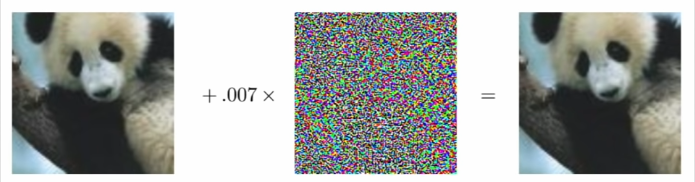
\includegraphics[width=12cm]{img/panda-adversary.png}
    \caption{Adversarial Example}
    \label{fig:panda}
\end{figure}

Here, the panda which was initially classified with a high degree of confidence was classified as another animal with an even higher degree of confidence later.

This vulnerability isn't limited to deep learning though. Even simple machine learning algorithms are susceptible to such behaviour. The lecture above shows how a linear softmax model was tricked such that the numbers (from the MNIST dataset) was tweaked and the trained model predicted the digital '9' to be any other digit. The tweaks did not substantially change the image at all. The same goes for logistic regressions and decision trees.

The initial explanation of this was that of overfitting, and the model fits the training set well and does randomly on the test set. But it was seen that this was not the case. The new idea was that of underfitting - like with linear models.

In fact, modern deep nets are like piecewise linear functions. Or rather, the mapping of the input to the output is linear - not parameters to output (which is non linear). This is interesting because with a linear model - there is a very high probability for a class assigned to points that aren't near our dataset to begin with. Hence, on such unseen data we are very confident about the class of our item. 

It's very easy for us to choose pertubations that choose the true class of an object. When making adversarial examples, we have to be careful to choose instances that retain the true class but give us a mismatch. It can be shown that for very small changes in our image vectors, the changes can have massive impact. 

\section{Fast Gradient Sign Method}

\textbf{Fast Gradient Sign Method} is a way to generate adversarial examples to attack a model by maximising a modified loss function that minimizes the distance between two images. The sign of the negative gradient of loss section determines how we want to change our image.

The adversarial examples were shown to exist in linear subspaces rather than in tiny groups which might have been the case with overfitting.   

To make things more interesting, it was shown that models in fact almost misclassify everything. That is, when you shift the input space for train and test data, the model performs very poorly. The lecturer goes on to show that for noise input, the CIFAR classifier gave high confidence for a lot of the images - one in four was considered to be an airplane - the lowest probability for any class. Ideally, we want to be able to know nothing or some abiguity from the classifier when fed noise. 

\section{Transferability}

 "Adversarial examples that affect one model often affect another model, even if the two models have different architectures or were trained on different training sets, so long as both models were trained to perform the same task.  An attacker may therefore  train  their  own substitute model,  craft  adversarial examples against the substitute, and transfer them to a victim model, with very little information about the victim" - from a \href{https://arxiv.org/pdf/1605.07277.pdf}{transferability of adversarial examples}.
 
 If the attacker doesn't have access to the target model itself - or have any knowledge of how it was obtained. We can train our own model and use that. If we don't have a training set, we can just send that training set as queries to the target model and use the label that is given. Making adversarial examples on our own model can then be found to transfer on the target dataset as well. 
 
 \textit{Optical illusions are like adversarial examples for humans} Perhaps this is indicative of a different learning method in our brains that the current deep learning methods.
 
 Training on adversarial examples has been found to reduce overfitting and helps generalize and improve the performance of models. Adversarial training introduces pertubations to the images to augment our training set. Even with unlabelled data, we tell the model to consider the same class as the unmodified image. 
 
 In short, adversarial training provides regularization and semi-supervised learning improvements.
 
 \subsection{Regularization}
 
 Adversarial regularization is a technique that aims to improve the robustness of models for pertubed examples. It 
 
 \section{Generative Adversarial Networks (GAN)}

Explanation from \href{https://towardsdatascience.com/progan-how-nvidia-generated-images-of-unprecedented-quality-51c98ec2cbd2}{this article}.
 
Generative Adversarial Networks (GANs) have been around for a few years now. They were introduced in a now famous 2014 paper by Ian Goodfellow and colleagues at the University of Montreal, and have been a popular field of inquiry ever since.

In short, GANs are a type of generative model that attempts to synthesize novel data that is indistinguishable from the training data. This is a form of unsupervised learning. It has two neural networks, locked in competition: a generator, that is fed a vector of random numbers and outputs synthesized data, and a discriminator, which is fed a piece of data and outputs a probability of it being from the training set (as opposed to synthesized). In other words, the generator creates “fakes”, and the discriminator attempts to distinguish these “fake” samples from the “real” ones.

\chapter{Generative Models}

In unsupervised learning, we have no labels, just data!. This could include clustering tasks, dimensionality reduction, feature learning (has an encoder and a decoder with the features in between, we want to recreate the input image out of the decoder - autoencoder), density estimation. Unsupervised learning is interesting because there are no labels, easier to gather data. It is a relatively unsolved research area. If solved, we can ideally understand the visual structure of the world. 

Generative Models are a class of models for unsupervised learning, where we are trying to create data from the same distribution of the input/training data. They address the problem of density estimation. There are various flavours to this

\begin{itemize}
    \item Explicit density estimation: explicitly define and solve for $p_{model}$
    \item Implicit density estimation: Here, we let the model figure out the density on its own.
\end{itemize}

This is an extremely interesting application because it can create new images, and even for reinforcement learning with time series data. \href{https://arxiv.org/pdf/1701.00160.pdf}{This} tutorial by Ian Goodfellow seems to be a very comprehensive lecture on GANs, and touches on various generative models and the underlying concepts.

\section{PixelRNN and PixelCNN}

They are fully visible belief networks that explicit density model. Here, the images generated use a chain rule as the product of all the pixels before it. or

\begin{equation}
    p(x) = \prod_{i=1}^np(x_i|x_1, \hdots, x_{i-1})
\end{equation}

where $P(x)$ is the likelihood of the image x. We then look to maximize the likelihood of this training data under this defined density. Note that this is a really complex distribution, and we can model these using neural networks. Even if we use a neural network, we need to have an ordering for pixels. 

PixelRNN was a model proposed in 2016 that defines a way to set up and optimize this problem: generate image pixels starting from a corner, and sequentially generate the pixels by moving horizontally and vertically one step at a time. This uses a RNN with LSTM. This is very slow since it is very sequential - iterative model.

PixelCNN has a similar setup as PixelRNN, but here we use a CNN to model dependencies and use a CNN over a context region. Here, interestingly, we use our input data and have a RGB value for each pixel. So the CNN is tasked with minimizing the softmax loss such that it tries to match the input RGB value. Note that this isn't supervised learning since there are no new labels (we didn't collect anything!). Here, training is faster since we can parallelize convolutions since context region values known from training images. Generation time is still slow though since we must proceed sequentially.

These models don't work particularly well but they sort of make natural looking images. 

\section{Variational AutoEncoders (VAE)}

PixelCNN uses a tractable density function, optimizing the likelihood of a density function. 

VAEs use an intractable density function with latex $z$. This function cannot be optimized directly, we derive and optimize on the lower bound of the likelihood instead. 

\subsection{Autoencoders}

Autoencoders are an unsupervised approach for learning a lower-dimensional feature representation from unlabeled training data. Let our input be $x$ and the features $z$. Generally, $z$ is generally lower dimension than $x$. This is because we only want the good features of the data. We then use a decoder that should be able to use these features to recreate the image $\hat{x}$. The encoder takes the image to lower dimension and the decoder takes it to a higher dimensional feature. This can then use a loss function to minimize distance between $x$ and $\hat{x}$.

We can also use the features that we get to train a classifier in a supervised learning tasks.

Variational Autoencoders are a probabilistic "spin" on autoencoders to sample from the model to generate data. Here, we have our features $z$ that we sample from (the true prior- $p_{\theta^*}(z)$). We want to generate the image $x$ by sampling from the true prior or $p_{\theta^*}(x|z^{(i)}$. We want to estimate the true parameters $\theta^*$ of the model. 

\textbf{How do we train this?}

Ideally, we'd like to maximize the probability $p_{\theta}(x)$ which is:

\begin{equation}
    p_{\theta}(x) = \int p_{\theta}(z)p_{\theta}(x|z)dz
\end{equation}

The problem with this is that the integral is hard to compute and use for gradients. Hence, this can't directly optimise this. But, in addition to using a decoder network, if we have an encoder network.

\part{Robot Operating System}

\chapter{Robot Operating System (ROS)}

With ROS, we needn't write drivers for our robots and is an abstraction of the hardware and low level device control. It is essentially a peer to peer connection (not server-client). Nodes can share information among themselves by identifying as a subscriber and a publisher. It is also multilingual (C++ and Python codes can interact) as communication occurs via messages. ROS is also distributed across systems and has a large open source community. The commands haven't really been written here.

\href{https://jack-kawell.com/2019/06/24/setting-up-a-ros-development-environment-in-windows/}{This} was a very simple tutorial on setting up ROS for WSL.

\href{http://wiki.ros.org/ROS/Tutorials/}{This tutorial on using ROS} covers everything in sufficient detail. This chapter doesn't really do the concept justice - just name drops some concepts really. I also liked the book 'ROS by Example' to see things working at a larger scale.

\section*{ROS Master}

ROS Master exists to store the addresses of the other nodes and helps nodes find each other, exchange messages or invoke services.

\section*{Nodes}

ROS nodes always register to the ROS master. Nodes are single purpose ecxecutable programs and contain main logic. \textit{rosnode list} will show list of active nodes. \textit{rosrun package\_name node\_name} will run the package on the node. 

\section*{Topic}

Each node publishes to a certain topic - to which other nodes can subscribe and then communication occurs over this topic. Hence, subsribers don't care about who is publishing but rather the topic itself. For example: If we have a camera that captures image and RGB information, this information could be required by various nodes such as odomtry, DL pipeline, etc, so these nodes can subscribe to a topic that the camera publishes to.

\section*{Messages}

Nodes communicate with each other by passing messages. A message is simply the communications that are exchanged over a topic.

\section*{Components on a Mapping Robot}

A robot is equipped with lidar, kinect, and odometry sensor. It will publish RGB information, depth information, and image information. This will be published so that an another node can process this information and form a synchronized image. A laser scanner and odometry will send information (these may have errors). \textit{rtabmap} a mapping algorithm will use these information and send map data to a top - an assembled point plot.

\section*{ROSBag Files}

Bags are a format for saving and playing back ROS message data. It is very useful for debugging. For instance, if have a self driving car, we don't want to use it everytime. With a ROSBag file we can recreate the conditions as earlier with the same timestamps as well. Hence it is suited for logging and recording datasets for later vizualization and analysis.

\section*{Creating ROS Workspace}

ROS codes should be maintained inside a catkin workspace. We make packages and nodes inside this workspace. You have to make these packages later to build these packages to binaries that can be executed.

\section*{Some Packages}

\subsection*{TF Transformation Package}

This is a package that lets us keep track of multiple coordinate frames. Obviously, for various components of a robot, each will likely work with it's own frame of reference - relevant to itself. This maintaines a relationship between coordinate frames in a tree structure buffered in time. We can then use the API to transform points and vectors between coordinate frames.

\subsection*{TF Listener and Broadcaster}



\part{Rigid Body Transformations and Projective Geometry}

\chapter{Introduction to Photogrammetry}

If recapping - skip to the "Better Explanation" section.

This chapter was taught using Computational Photogrammetry by Cyrill Stachniss.

Computer Vision came into being because cameras existed that could image things. Let's consider a pinhole camera - it assumes that all rays will come through the pinhole and it can use these rays to project an image onto another screen. The image is hence, a projection of points in a 3D world to a 2D surface. Camera center is the intersection point of the rays. The back wall is the image plane. The distance between the camera center and image plane is the camera constant.

We'll assume that all our cameras for the next sections are pinhole cameras. 

\textbf{Geometry and Images}

Pinhole cameras have some properites: The straight lines are preserved, lengths are not preserved, and angles between lines change. Additionally, parallel lines may intersect depending on the angle at which the image is taken.

Image rectification is a transformation process used to project images onto a common image plane. Photogrammetry deals with such problems - the relationship between the object in the scene and the object in the image, the image and the rays in the object, the orientation of cameras in the scene, and infer geometry of an object or a scene given an object.

Photogrammetry is hard because information is lost when a scene is projected onto a surface by a camera. There is a loss of depth and 3D information cannot be recovered from this information alone - additional information required. 

\textbf{Vanishing Points}

Parallel lines aren't always parallel if taken at an angle and they intersect at a vanishing point - at infinity. This information cannot classically be represented using cartesian coordinates $(x, y)$. Euclidian geometry is suboptimal to describe the central projection. Projective geomtry is an alternate representation of geometric objects and transformations. With projective geometry, the math becomes simpler

Hence, we need a new representation for coordinates which is homogeneous coordinates.

\section{Homogeneous Coordinates}

Homogenous coordinates are for projective geomtry just as cartesian coordinates are for Euclidian geometry. Formulas involving H.C. are often simpler than in the Cartesian world. The points at infinity can be represented using finite coordinates. Further, complex projective transformations can be represented using a single matrix! 

"The  ideas and notation of projective geometry are central to an analysis of multiple view geometry.For example, the use of homogeneous coordinates enables non-linear mappings (such as perspective projection) to be represented by linear matrix equations, and points at infinity  to  be  represented  quite  naturally  avoiding  the  awkward  necessity  of  taking limits." from \href{https://github.com/pranjals16/cs676/blob/master/Hartley\%2C\%20Zisserman\%20-\%20Multiple\%20View\%20Geometry\%20in\%20Computer\%20Vision.pdf}{this}.

\textbf{Notation}

\begin{itemize} 
    \item Point $\chi$: In homogenous it is x, in euclidian $x$
    \item Line in homogeneous coordinates is l.
    \item Plane in homogenous coordinates : A
\end{itemize}

The representation x of a geometric object is homogenous if x and $\lambda$x represent the same object for $\lambda \neq 0$. H.C uses a n+1 dimensional vector to represent the same point:

\begin{equation}
    x = \begin{bmatrix}
    x \\
    y
    \end{bmatrix} \text{ and x = } \begin{bmatrix}
    x \\
    y\\
    1
    \end{bmatrix}
\end{equation}

Note that in general for a point $x = (x, y)^T$ and a line $l: ax + by + c = 0$ satisfies $x \cdot l = 0$. 

\begin{figure}[t]
    \centering
    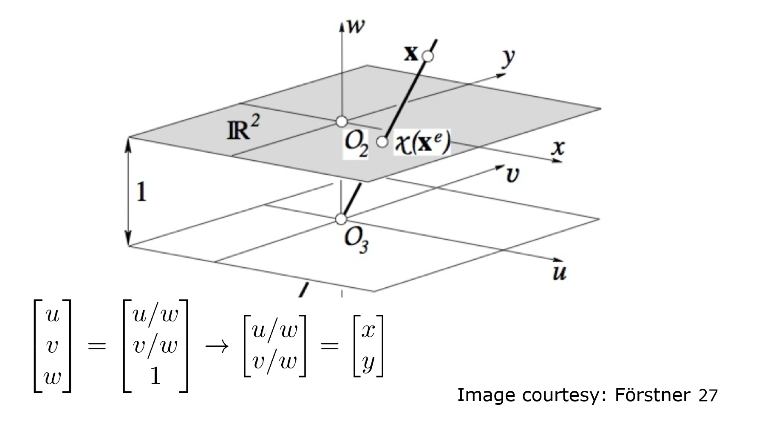
\includegraphics[width=10cm]{img/homogenous-eucclidian.png}
    \caption{Homogeneous Coordinates Representation/Visualization}
    \label{fig:hc}
\end{figure}

Before coming to the image notation, it is useful to look at section 2.2.1 of \href{https://github.com/pranjals16/cs676/blob/master/Hartley\%2C\%20Zisserman\%20-\%20Multiple\%20View\%20Geometry\%20in\%20Computer\%20Vision.pdf}{Multiple View Geometry in Computer Vision by Hartley, Zisserman}. The book is a great source of information. I would've written that explanation myself but it's hard to do it better than that.

Summary: A point in a 2D plane can be represented as a 3D column vector, and when multiplied by a constant k, it still represents the same point - just on the line that may be scaled by the same constant. It is natural, therefore, to consider the set of vectors $(kx, ky, k)^T$ for varying values of $k$ to be a representation of the point $(x, y)^T$ in $R^2$. Thus, just as with lines, points are represented by homogeneous vectors. An arbitrary homogeneous vector representative of a point is of the form $x=(x_1,x_2,x_3)^T$, representing the point $(x1/x3,x2/x3)^T$ in $R^2$. 

Refer to figure \ref{fig:hc}.

Let us assume that we have a 2D plane that is our image. Now, different points on this image can be visualized to have certain rays passing through it. If we look at the diagram, the point x is a point on the ray that can be represented with our scaling factor/H.C. value. The origin $O_3$ is where the rays originate from (camera center). In fact, we cannot have this origin point in our coordinate system since if the image has this point, then there is no direction for any of the rays. Hence homogenous coordinates of a point $\chi$ in the plane $R^2$ is a 3-dim vector.

\begin{equation}
    \chi: \; x = \begin{bmatrix}
    u/w \\
    v/w 
    \end{bmatrix}
     \text{ with $w\neq 0$ }
\end{equation}

Now, if $w$ is 0, then that is essentially our understanding of a point at infinity in the direction of $u$ and $v$ (notice how $u/0$ is infinity!). The projective plane (the grey plane) contains all points $\chi$ of the Euclidian plane $R^2$ with $x = [x, y]^T$ expressed through a 3 valued vector and all points at infinity (x = $[x, y, 0]^T$ except $[0, 0, 0]^T$).

Additionally, it can be seen that our homogeneous property is like the depth of the point/distance from camera center.

\subsection{Representation of Lines}

Refer to slides 31+ \href{https://github.com/RoboticsIIITH/summer-sessions-2020/blob/master/lecture-slides/Computational\%20Photogrammetry/Projective\%20Geometry\%20Lecture\%201.pdf}{here}.

There is a duality between lines and points when we talk about them (they are both 3D vectors!!). 

\subsection{The Better Explanation}

I did not understand any of this until I read \href{https://pointatinfinityblog.wordpress.com/2016/04/11/points-at-infinity-i-projective-geometry/}{this resource} by points at infinity. It is very well-written but a gist could be:

\begin{enumerate}
    \item We can look at projective planes (which we represent with homogeneous coordinates) as a window through which we see the 3D world. Previously, we used the idea of a pinhole camera. Rather than that, imagine that you are looking at a real building or so. Now, if we had to paint this/capture this image, we will trace a line from a point on the building to our eye. This is a line in 3D euclidian space. This line becomes a point in projective $P^2$ space!
    \item Note that if we know a point on a line, if we multiply it with a scalar, we get a new point on the line! ($x + y + z = 0 \implies \alpha(x+y+z)=0)$. Hence, the entire set of points in 3D space that lie on the same line from the building to our eye can be represented by a single line which in turn is a point in projective plane!
    \item Now if a line in 3D is a point in projective plane, a plane in 3D is a line in projective plane. Imagine this this way: when we trace a line on our image of a building, we can imagine that we are drawing a line on the window through which we see the building. Further, this line can slowly be moved back (like the points on the line that connected our eye and the building). Now, we see that the line on our image, when extended became a plane! The representation for the line is also with a 3D vector. 
    \item We have already seen that for a line (a 3D euclidian line) represented by $(a, b, c)$, the point in projective plane can be represented with $(a, b, c)$ as well but for ease, we tend to use $(a/c, b/c, 1)$. Further, if we capture the image, the coordinate for this point can be imagined as $(a/c, b/c)$.  
    \item Points at 3D: The main reason to move towards projective plane is to introduce the idea of parallel lines convering at infinity. When we have a line with $c=0$, this means that our image point is $\infty, \infty)$ or rather, the line ends at infinity! This is precisely why parallel lines intersect at infinity in a projective plane! 
\end{enumerate}

\subsection{Intersecting Lines}

If we have two lines $l, m$ that intersect at a point $x$, then x will satisfy both line equations or:

\begin{equation*}
\begin{bmatrix}
l\cdot x \\
m\cdot x
\end{bmatrix} = \begin{bmatrix}
0 \\
0
\end{bmatrix}
\end{equation*}

\subsubsection{Cramer's Rule}

Given a system of linear equations, Cramer's Rule is a handy way to solve for just one of the variables without having to solve the whole system of equations. If we have a system of equations, let $D$ be the coefficient matrix's determinant. $D_X$ is the determinant of coefficient matrix which has the solution vecctor in the $x-\text{column}$. As per cramer's rule, $x = D_x / D $. Now, for this $2 \times 2$ system, we will find that $D_1 = l_2m_3 - l_3m_2$ and $D_2 = l_3m_1 - l_1m_3$ and $D_3 = l_1m_2 - l_2m_1$. Looking at this closer will tell us that the coordinate/point x is actually $l \times m$ (the cross product)!.

Similarly, we can show that the line that passes through two points is represented by the cross product of these two points. 

\subsection{Parallel Lines and ideal points}

Read section 2.2.2 of the multi view book to look at how parallel lines intersect at infinity! There is honestly nothing better to understand. I'm also very dead atm.2

\chapter{Photogrammetry - II}

With transformations we want to transfer coordinates from various systems to another. From the world coordinate system, to the camera coordinate system, to the image coordinate system.

In the pipeline of transforming coordinates, there are extrinsics and intrinsics. The extrinsics describe the pose of the camera in the world. Intrinsic parameters describe the mapping of the scene in front of the camera to the final image. 

\textbf{Key Convention Point}

In a regular pinhole camera, the image is formed BEHIND the camera center. This is obviously how physics works but for the near entirety of this field, we will consider the image formed in front of the camera center. This is purely to make representation and math simpler. Obviously, this doesn't change anything or invalidate "normal" math as the figures will actually be congruent.

\section{Camera Intrinsics and Extrinsics}

Extrinsic parameters describe the pose of the camera in the world. On the other hand, intrinsics describe the mapping of the scene imaged to the the image taken.

\textbf{Extrinsics}

There are 6 parameters to represent the extrinsics - 3 for position + 3 for direction. The translation between origin of world and camera center represents the transformation $X_O = [X_0, Y_0, Z_0]^T$. Then, there is a rotation matrix $R$ that represents the direction of the camera. 

\textbf{Intrinsics}

The process of projecting points from the camera to the image and to the sensor requires intrinsics. We come across more of this later.

\subsection{Calibration}

Quite often, we read that a camera has to be calibrated prior to use. When calibrating a camera, we are trying to estimate some parameters - intrinsics. These parameters are critical to processing our image such as correcting lens distortion, determining the camera's location and so on.

\begin{figure}[h]
    \centering
    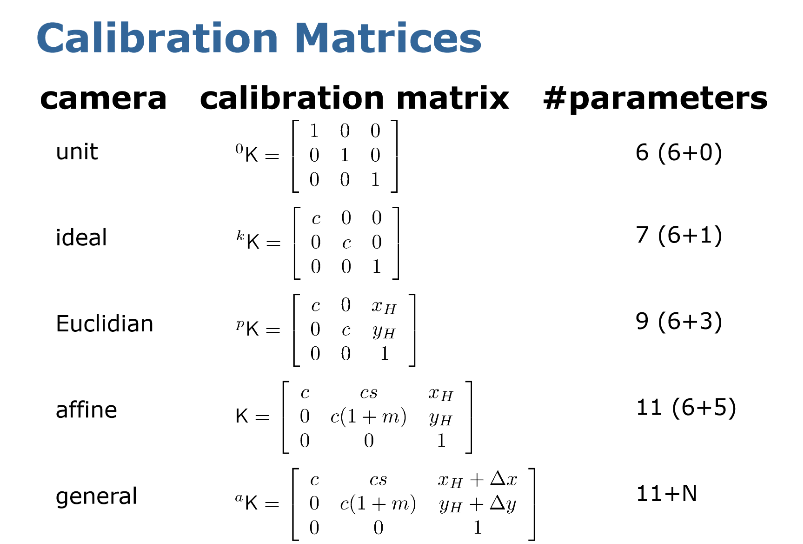
\includegraphics[width=12cm]{img/calibration-matrices.png}
    \caption{Calibration Matrices}
    \label{fig:calibration}
\end{figure}

The image \ref{fig:calibration} is useful to see what various calibration matrices we have. Some of these will be introduced later. 

\section{Projection Matrix}

On multiplying the projection matrix with the camera coordinates, we obtain the projected image coordinates. This projection matrix is a camera instrisic that is defined with the focal length values. 

I didn't write this section until after the next lecture. Look at the section on Camera Modelling in chapter 13 to read more about how projections are represented.

\section{Transformations}

Transformations include shearing, rotation, scaling, each of which can be represented using a single matrix.

\subsection{2D Rotations}

\begin{equation}
    R = \begin{bmatrix}
    \cos\theta & -\sin\theta \\
    \sin\theta & \cos\theta 
    \end{bmatrix}
\end{equation}

This transformation is orthonomal such that $R^{-1}=R^T$. Here, the column vector correspond to the new axes that are formed after rotating that particular vector.

\subsection{3D Rotation}

With 3D rotation, we can rotate the body along any particular axis. So, when we rotate along the $z$ axis for instance, it means that you "fix" the z axis and move the $x$ and $y$ axes. Hence, the $z$ coordinate doesn't change but the X-Y coordinate changes - just as they would in the 2D rotation case. Hence, the rotation matrix is:

\begin{equation}
    R_{z}(\theta) = \begin{bmatrix} 
    \cos\theta & -\sin\theta & 0 \\
    \sin\theta & \cos\theta & 0 \\
    0 & 0 & 1
    \end{bmatrix}
\end{equation}

In general, the matrix can be seen as a table where the column headers are $x, y, z$ of the new frame and the rows are the initial frame. The elements in $j^{th}$ column and $i^{th}$ row is in fact the PROJECTION of the $j^{th}$ point (can be seen as a vector from origin) on the $i^{th}$ axis - always assuming the unit vector (why should we consider scaling here anyway).

Look up the rotations along other axes. We needn't have just rotations along one axis though. But, it is still simple! Let's assume that we have some rotation in mind that is not along a particular axis. We can make the same rotation along one axis and then along another axis. This is hence, a product of two rotations along the axis. We can string together various axis rotations in such a manner to get any general rotations. 

Rotations are always relative to the current frame.

Rotations in real life are quite interesting as often they do not just "rotate" an object, but also change the direction in which a component is pointing at. Imagine a robotic arm that is spray painting. If we didn't consider direction, on rotating the arm, it would paint in a different direction altogether.

\subsection{Scaling}

Scaling is obviously just stretching vectors along a particular direction. For instance, $x'=sx$. This can be represented by a matrix :

\begin{equation}
    \begin{bmatrix}
    x \\
    y\\
    z\\
    \end{bmatrix}' = \begin{bmatrix}
    s & 0 & 0 \\
    0 & u & 0 \\
    0 & 0 & t \\
    \end{bmatrix} \begin{bmatrix}
    x \\
    y\\
    z
    \end{bmatrix}
\end{equation}

This will not change parallelism, ratio of lengths in any direction.

\subsection{Shearing}

With shearing, we are essentially stretching a vector along a certain direction. Note that we are stretching, not displacing. Now, when we are stretching a square on a 2D plane, assume that there is a resulting parallelogram. Clearly, all points in the square were not shifted equally. In fact, the greater the $y$ coordinate, the greater it was shifted on the $x$ axis. This is precesily how we write our shearing matrix:

\begin{equation}
    \begin{bmatrix}
    1 & x_y & x_z \\
    y_x & 1 & y_z \\
    z_x & z_y & 1
    \end{bmatrix}
\end{equation}

\subsection{Reflection}

With reflection, we neflect around a particular axis. Hence, we negate along a particular axis. So the matrix could look like:

\begin{equation}
\begin{bmatrix}
-1 & 0 & 0\\
0 & -1 & 0 \\
0 & 0 & 1
\end{bmatrix}
\end{equation}

\subsection{Translation}

Translation is the only transformation that is represented by a particular vector. But, with homogeneous coordinates we can represent it as a matrix.

\section{Frames}

In a lot of places, we refer to transforming points and frames. It's intuitive to think of frames as the coordinate system. Hence, transformations on our frame shifts our coordinate system. The origin and axes change with the transformations.

\section{Axis-angle representation}

This is a different way to represent rotations using a pair of vector and angles. He did not explore this in more depth, but it helps avoid some problems with other representations. For example [0,0,30] indicates along [0,0,1] axis, rotate by 30 degrees. \textit{I think he said that axis angles are euclidian - this is huge since rotation matrices aren't euclidian!}

\part{Multiple View Geometry}

\chapter{Feature Matching and Extraction, Camera Modelling}

The first task when we get images from various images is to extract features from these images and intersect these. So, an image of a cat from various images can be identified to be the same. Doing so will also enable us to triangulate among other applications. This chapter will also look at transformations. A feature is a piece of information which is relevant for solving the computational task related to a certain application. Features may be specific structures in the image such as points, edges or objects. Features may also be the result of a general neighborhood operation or feature detection applied to the image. The features can be classified into two main categories:

There are multiple kinds of geometry - single view, two view (\href{https://web.stanford.edu/class/cs231a/course_notes/03-epipolar-geometry.pdf}{epipolar}, projective reconstruction) where we see stereo matching (given two images, reconstruct the whole scene).

Additionally, with multiple view geometry we can stitch images together for instance - just as in panaroma.

\section{Feature Matching and Extraction}

\subsection{Detector Algorithms:} Algorithms that find interest points in an image. The interest points could be corners of an image (things which are flat and continuous surfaces may not be of interest - we need uniqueness). Now, if we use corners, they are likely unique and can be identified across images - matched in different frames. eg: Harris corner detector

\subsection{Descriptor Algorithm:} Algorithm that encodes features of the points that are identified by the detector algorithm. eg: SIFT descriptor (SIFT includes a detector as well as a descriptor)

\subsection{Image Gradients}

The image gradient along a direction, we convolve the image I with various kernels that represent the gradient along a particular direction. Hence, we are left with gradients along various directions. For instance:

\begin{equation*}
    I_x = \begin{bmatrix}-1 & 0 & 1\end{bmatrix}\cdot I
\end{equation*}

\begin{equation*}
    I_y = \begin{bmatrix}-1 \\ 0 \\ 1\end{bmatrix} \cdot I
\end{equation*}

\textbf{Gradient magnitude and direction:}

\begin{equation*}
    I_{\theta} = \tan^{-1}(\frac{I_y}{I_x})
\end{equation*}

\subsection{Harris Corner Detector} 

\begin{figure}
    \centering
    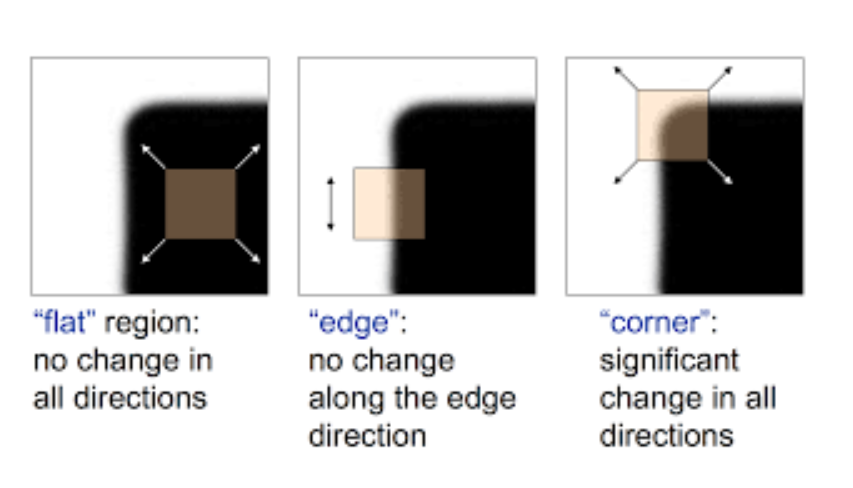
\includegraphics[width=10cm]{img/harris-corner.png}
    \caption{Harris Corner Detector}
    \label{fig:harris}
\end{figure}

The corner detector is looking for significant changes in all directions. A flat surface would have no change across any direction and a straight line feature would only change in one direction. With more directions that have gradients, we can uniquely identify it.

\subsubsection{Example of descriptor}

In a descriptor, we divide the image into several squares. For each of these squares, we will calculate the gradient and obtain the direction. Now, depending on the weight of the gradient along various directions, we will create a histogram for the gradients and choose the largest one. Now, these histograms apply only for a certain subblock of the image. If we club these histograms together, we get a feature map.

\href{https://medium.com/data-breach/introduction-to-sift-scale-invariant-feature-transform-65d7f3a72d40}{\textbf{SIFT}} is a very popular feature extraction algorithm.

\section{Frame Transformations}

The transforms that we were looking at earlier were point wise transforms. Now, we will be looking at frame wise transformations largely.

\begin{equation*}
    {}^WX=T^{World}_{Camera}{}^CX
\end{equation*}

Here, $T^{World}_{Camera}$ is the transformation that goes from world frame to camera frames. Or, it transforms from camera to world point system. Frame and point transforms are \textbf{inverse} of each other. 

\textbf{Frame perspective vs point view}.

Now when considered as frames, we multiply the transformation matrix to a point (represented relative to camera). This transformation essentially changes the basis - representing our point in a new frame. On the other hand, if we imagine the matrix as just a matrix, and consider the same basis, we can consider this to be a point transformation. But, the point transformation is in the opp direction of frame transformation.

\begin{figure}[h]
    \centering
    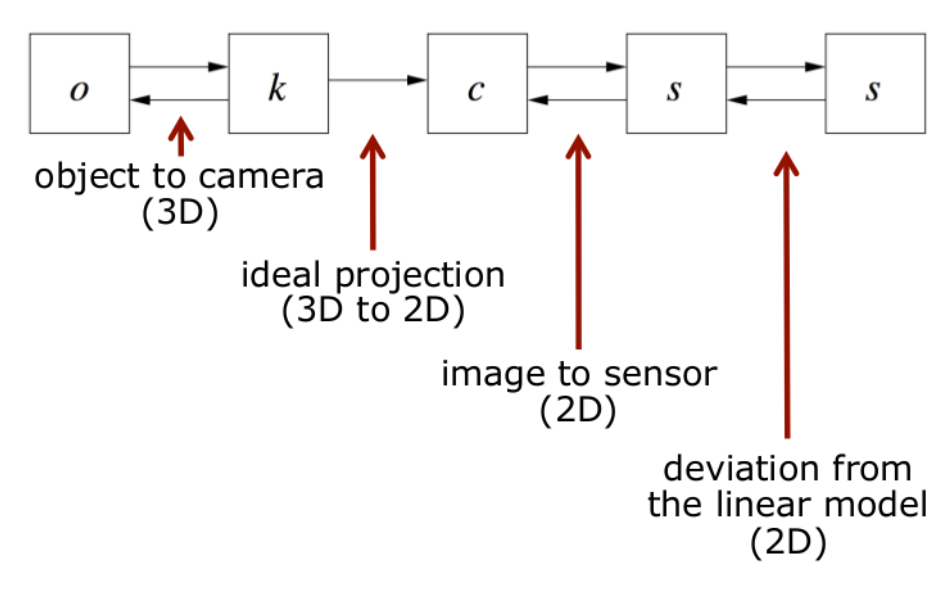
\includegraphics[width=12cm]{img/camera-pipeline.png}
    \caption{Pipeline of Transformations}
    \label{fig:pipeline}
\end{figure}

In image \ref{fig:pipeline}, first we transform from world frame to the camera frame (is invertible as inverse transformation matrix will take us from camera frame to world frame), then when we take an image, it is a projection (not invertible since we lose depth information).

Sensor will take it to an ideal space which the pinhole camera cannot take care of alone. The sensor coordinate system will hence take care of these transformations. 

\subsection{Making Transformations}

Now, we will frequently need to make transformations that rotate our camera, the object captured by the camera and so on. Since we represent everything with matrices, we also represent these transformations with matrices. How do we multiply this? There are two options: Post or pre multiplication. In general, if we post multiply, it means that the transformation was applied around the current frame. On the other hand, pre multiplying the matrix means we transform around the new frame of reference.

Look at slides \href{https://github.com/RoboticsIIITH/summer-sessions-2020/blob/master/lecture-slides/Multiple\%20View\%20Geometry/lecture-1/MVG_Session_1.pdf}{23+}. Here we have a matrix that represents the frame (by convention really) along with a camera center. Camera center - perpendicular distance between principal axis from camera center to the center of image plane.

\textbf{Something to explain slide 27 of \href{https://github.com/RoboticsIIITH/summer-sessions-2020/blob/master/lecture-slides/Multiple\%20View\%20Geometry/lecture-1/MVG_Session_1.pdf}{Rahul's slides}}

\section{Camera Modelling}

A camera's properties can be represented using a single matrix. We will use a pinhole camera here. So far, we have considered homogenous coordinates to ONLY look at points on our images. We always mentioned that these points corresponded to lines in the 3D system. Now, we will represent image points and the real world points in homogeneous coordinates:

\begin{equation*}
    \begin{bmatrix}
    X \\
    Y \\
    Z \\
    1
    \end{bmatrix}\longrightarrow \begin{bmatrix}
    fX \\
    fY \\
    z
    \end{bmatrix} = \begin{bmatrix}
    f & 0 & 0 & 0 \\\
    0 & f & 0 & 0 \\
    0 & 0 & 1 & 0 \\
    \end{bmatrix} \begin{bmatrix}
    X \\
    Y \\
    Z \\
    1
    \end{bmatrix}
\end{equation*}

where f is the focal point essentially. Look at the following image to understand the coordinates:

\clearpage

\begin{figure}[t]
    \centering
    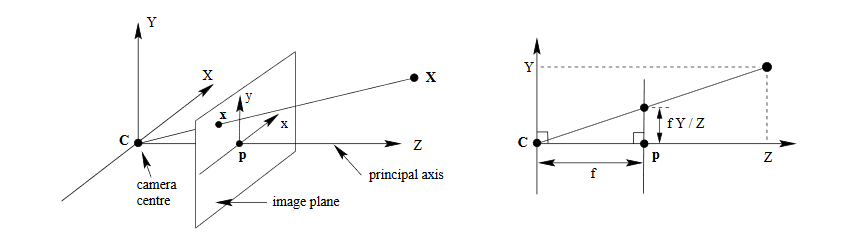
\includegraphics[width=12cm]{img/pinholecamerageometry.png}
    \caption{Pinhole Camera Geometry}
    \label{fig:pinhole-cam-geo}
\end{figure}

The matrix in this above expression can be written as $diag(f,f,1)[I|0]$, where $I$ is a $3\times3$ matrix followed by another $0$ column vector. By convention, let $X$ be the world point, and $x$ be the image point. We'll refer to the above transformation matrix as the camera projection matrix $P$. Hence,

\begin{equation}
    x = PX
\end{equation}

The above expression assumed that the origin of coordinates in the image plane is at the principal point. 

\begin{figure}
    \centering
    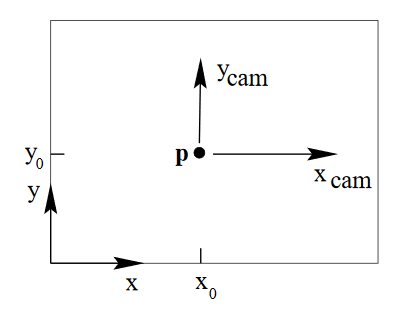
\includegraphics{img/camera-shift.png}
    \caption{Camera Shift}
    \label{fig:camera-shift}
\end{figure}

Hence, the image points will have a certain offset. Now, we will rewrite the projection matrix as follows:

\begin{equation*}
    \begin{bmatrix}
    X \\
    Y \\
    Z \\
    1
    \end{bmatrix}\longrightarrow \begin{bmatrix}
    fX \\
    fY \\
    z
    \end{bmatrix} = \begin{bmatrix}
    f & 0 & p_x & 0 \\\
    0 & f & p_y & 0 \\
    0 & 0 & 1 & 0 \\
    \end{bmatrix} \begin{bmatrix}
    X \\
    Y \\
    Z \\
    1
    \end{bmatrix}
\end{equation*}

This matrix is called the camera calibration matrix and $x = K[I|0]X_{cam}$. The camera here is located at the center of the euclidian coordinate system. 

The parameters of the matrix K are called the intrinsic parameters of the camera. Now, we can choose to change the camera orientation and position in the world coordinate system.

If we assume that the position of the camera center in the world coordinate frame is $\hat{C}$, and we rotate the camera coordinatie frame. This is a rotation and translation essentially.

Putting this together, we find that:

\begin{equation}
    x = KR[I|-\hat{C}]X
\end{equation}




\chapter{Camera Calibration Methods}

As seen earlier, camera calibration is the process of determining the intrinsic of a matrix. This is done after obtaining data correspondences between the world coordinate system and the image system.

\section{Direct Linear Transform}

Most of this has been taken from Cyril Stachniss' slides which may be found \href{https://github.com/RoboticsIIITH/summer-sessions-2020/blob/master/lecture-slides/Multiple\%20View\%20Geometry/lecture-2/pho1-16-DLT-calibration.pptx.pdf}{here} and the video \href{https://www.youtube.com/watch?v=3NcQbZu6xt8}{here}.

The task is to estimate the 11 elements of P when given 3D coordinates of object points in world frame $X_i$ and image pixel coordinates $x_i$. This essentially means that we have an uncalibrated camera!

Hence, $x_i = PX_i$ where we map a world coordinate to a pixel coordinate. When we know the world coordinate, the mapping in the image, our task is to calculate the matrix $P$. 

What is in the matrix P? $KR[I_3|-X_0]$ where $X_0$ is the location of the camera, $R$ is the orientation, and $K$ is the intrinsics which store camera calibration properties. Hence, the projection matrix contains intrinsics and extrinsics. There are 3 translation parameters in $X_0$, 3 in rotation, and 5 in intrinsics.

There are a lot of unkowns here, so how much information is required? We have 11 unknowns, and for each point, we get two equations. That is,

\begin{equation}
    \begin{bmatrix}
    x \\
    y\\
    1
    \end{bmatrix} = P\begin{bmatrix}
    X \\
    Y\\
    Z\\
    1
    \end{bmatrix}
\end{equation}

On solving this, we'll get a solution for $x$ and one for $y$. Hence, we will need around 6 points (6*2=12) to obtain the matrix.

If we had a calibrated camera, we have just 6 unknowns and can make do with just 3 points - using spatial resection.

Direct Linear Transform lets us compute this matrix and assumes an affine system - no non-linear noise on the image. Let us make the rows in our projection matrix a vector. Hence,

\begin{equation}
    x_i = \begin{bmatrix}
    A^T\\
    B^T\\
    C^T
    \end{bmatrix}X_i = \begin{bmatrix}
    A^TX_i\\
    B^TX_i\\
    C^TX_i
    \end{bmatrix}
\end{equation}

In the end, we want to represent points back in euclidian coordinates. Hence, we will set the third element in our image coordinate to 1. Or,

\begin{equation*}
    \begin{bmatrix}
    x_i \\
    y_i \\
    1
    \end{bmatrix} = \begin{bmatrix}
    u_i \\
    v_i \\
    w_i
    \end{bmatrix} = \begin{bmatrix}
    A^TX_i\\
    B^TX_i\\
    C^TX_i
    \end{bmatrix}
\end{equation*}

This would then imply that:

\begin{equation}
\begin{split}
    &x_i = \frac{u_i}{w_i} = \frac{A^TX_i}{C^TX_i} \\
    &x_iC^TX_i - A^TX_i = 0
\end{split}
\end{equation}

\begin{equation}
\begin{split}
    &y_i = \frac{v_i}{w_i} = \frac{B^TX_i}{C^TX_i} \\
    &y_iC^TX_i - B^TX_i = 0
\end{split}\end{equation}

Now, notice that we have a system of equations - where A, B, C are the variables. 

Let us combine the elements of A, B, C into a single matrix essentially giving us a 12 dim column vector (dimensions of P are $3\times4$ but there are still only 11 degrees of freedom). Let this vector be $p$.

Hence,

\begin{equation}
\begin{split}
    a_{x_i}^Tp=0 \\
    a_{y_i}^Tp=0
\end{split}
\end{equation}

where we define $a_{x_i}^T$ as the column vector = $(-X_i^T, 0^T, x_iX_i^T)^T$. Similarly, $a_{y_i}^T$ can be written as $(0^T, -X_i^T, y_iX_i^T)^T$. 

This will hold for all the data points that we have naturally. We can also stack these input elments such that:

\begin{equation}
    \begin{bmatrix}
    \vdots \\
    a_{x_i}^T \\
    a_{y_i}^T \\
    \vdots
    \end{bmatrix} p = 0
\end{equation}

\textit{Let $M$ be the matrix with $a_{x_i}, a_{y_i}$}.

\subsection{SVD Solution}

This is a homogeneous system of equations and can be solved using SVD. Solving this equation is equivalent to finding the nullspace of M. Ideally, we get 0 for $Mp$ but with so many datapoints, it is possible that it is not an exact solution. Hence, we just try to find the solution $p$ that minimizes the RHS. We shall use the least squared error - $w^Tw$ as the result to minimize.

Now, if we use SVD:

\begin{equation}
    M = U \times S \times V^T
\end{equation}

where S is a diagonal matrix with elements that are singular values. Ideally, we want a $0$ singular value. The matrix $V$ has vectors that correspond to each singular value. We will choose the one corresponding to the smallest singular value and call that our solution for $p$.

\textbf{Why do we do this?}

As per \href{http://newton.uam.mx/xgeorge/uea/graficacionII/homogeneous_equations.pdf}{this resource}, we can look at it this way:

\begin{itemize}
    \item If we have as many equations as unknowns, the diagonal matrix will have just one entry which is 0! The vector that corresponds to this will hence logically be the rightmost one in the $V$.
    \item For an over-constrained situation (more equations that unknowns), there is likely no exact situation (is what was mentioned earlier as well - we minimize the RHS). Hence, we are interested in the solution that minimizes the sum of squared errors - the smallest diagonal entry.
\end{itemize}

\textbf{There is not always a solution.} This is when all given points are on the same plane - we have a rank deficiency (entire rows/columns are the same!). There are also some other scenarios where this is possible. This situation is quite common when we take pictures of a wall - in which case we get a degenerate solution.  

\subsubsection{Obtaining K, R, $X_0$}

This is a tricky procedure. Look at \href{https://youtu.be/3NcQbZu6xt8?t=1543}{this video clip} to understand how it is done. It involves finding $X_0$ first by writing $P=H_{3\times3}h_{3\times1}$ where $H=KR$. Hence, $H^{-1}P = H^{-1}Hh = h$ is the camera center. Now, to find $K, R$, $K$ is a triangular matrix while $R$ is a rotation matrix. We can use QR decomposition to find these matrices then! 

\subsection{Lagrange Multiplier Solution}

The following section is largely from \href{https://github.com/RoboticsIIITH/summer-sessions-2020/blob/master/lecture-slides/Multiple\%20View\%20Geometry/lecture-1/MVG_Session_1.pdf}{Rahul Sajnani's slides}.

As mentioned earlier, we are trying to minimize the RHS. This RHS is written as $M\cdot p$ and the squared error is $(M\cdot p)^T\cdot(M\cdot p)$. This is subject to the constraint that $p\neq0$ obviously. Hence, we can solve this using lagrange multipliers.

We have the follow the optimisation problem:

\begin{equation}
    min_P(M\cdot p)^T\cdot(M\cdot p) - \lambda (p^T \cdot p -1)
\end{equation}

On differentiating the above function,

\begin{equation}
\begin{split}
    2\cdot M^T\cdot M\cdot p - 2\lambda\cdot p &= 0 \\
    (M^T\cdot M)\cdot p &= \lambda \cdot p
\end{split}
\end{equation}

Here, $p$ is the last eigenvector of $M^TM$ since the last eigenvector has the lowest variance along its axis. The explanation for this is similar to our choice with SVD.

\section{Zhang's Algorithm}

This is another algorithm that let's us calibrate the camera. In short, it uses multiple points from a planar object to estimate the calibration matrix. I didn't really study this in depth. Will add later if required.

\chapter{Epipolar Geometry, Stereo Cameras}

\href{https://web.stanford.edu/class/cs231a/course_notes/03-epipolar-geometry.pdf}{This} is a great resource to read up about epipolar geometry. 

Epipolar geometry is fascinating because when given images of an object from two views, we can calculate the world coordinates of the object using just the camera parameters and relative pose.

As per \href{https://github.com/pranjals16/cs676/blob/master/Hartley\%2C\%20Zisserman\%20-\%20Multiple\%20View\%20Geometry\%20in\%20Computer\%20Vision.pdf}{the textbook}, the epipolar geometry is the intrinsic projective geometry between two views.  It is independent of scene structure, and only depends on the cameras’ internal parameters and relative pose. This intrinsic geometry is described by a matrix known as the fundamental matrix F.

Here the parameters to consider are world points, image points, camera matrix, and relative pose. There are two application essentially:

\textit{The correspondence point is the set of points that are imaged onto diff images representing the same }

\begin{itemize}
    \item Search for given corresponding points given a certain feature. Known P, R, t and not correspondence point
    \item F and its decomposition given enough corresponding points.
\end{itemize}

\clearpage

\section{Intuition}

\begin{figure}
    \centering
    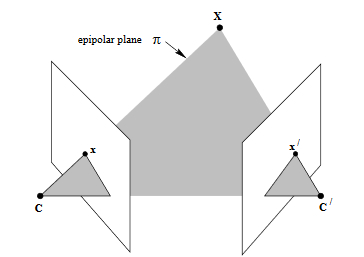
\includegraphics[width=12cm]{img/epipolar-1.png}
    \caption{Epipolar Plane Pictorially}
    \label{fig:epipolar}
\end{figure}

R, t are the relative transformation to get the second view from the first. Here, we have two cameras referring to a single point in the world coordinate system. But, imagine that we moved the point $X$ along the line described by $Cx$. The second camera would still capture the image. This essentially means that the possible world coordinates for a feature aren't unique! Looking closer at the image above, we can see that as we move $X$, we are tracing a line in the second image (with camera center $C'$). This is the epipolar line! Note that the epipolar line is a line on the image and hence a plane in euclidian space.

\textbf{Two Lines make a plane}

Intersection of the epipolar plane $\pi$ with the image plane (of the second camera) will give us the epipolar line. How do we form the epipolar plane? We need just 2 3D points to form a plane (take their cross product). We know cx already and cc' because the camera center has been transformed.

Let the epipolar line (on image 2) be represented as $l'$. To find the "stereo correspondence" for the point corresponding to x is what we need not cover the entire image plane but rather just the epipolar line.

Note that for every point on an image, we have an entire epipolar line on the other image.

An epipole is the point of intersection of the line joining the two camera centers with the image plane. The epipole in one image logically corresponds to the same point in the other image. 

\section{Fundamental Matrix}

"The fundamental matrix is the algebraic representation of epipolar geometry." As mentioned earlier, there was a mapping between point and epipolar line. This mapping is what is represented by the fundamental matrix. By multiplying the matrix with the point, we get a corresponding point in the other image.

\begin{figure}[h]
    \centering
    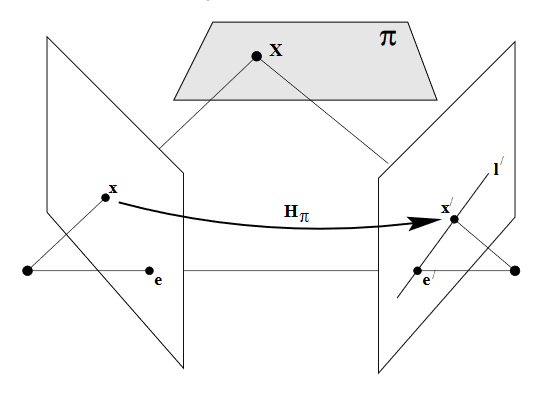
\includegraphics[width=12cm]{img/Fundamental_Matrix.png}
    \caption{A point $x$ in one image is transferred via the plane $\pi$ to a matching point $x'$ in the second image.}
    \label{fig:fundamental_image}
\end{figure}

\subsection{Geometric Derivation}

To derive F, we can look at it geometrically in two steps. From the book by Zisserman, the point $x$ is mapped to some point $x'$ in the other image lying on the epipolar line $l'$. This point $x'$ is a potential match for the point $x$. The second step, the epipolar line $l'$ is obtained as the line joining $x'$ to the epipole $e'$

Note that the points X, and x are projectively equivalent. Same for x'. Now, by projectivity theorem states that there exists a full-rank homography matrix $H_{\pi}$ such that:

There is a 2D homography from $x_i$ to $x_i'$.

\begin{equation}
    x' = H_{\pi}x
\end{equation}

Now, to get the epipolar line, we can take the cross product of two points which are on the line. If $e'$ is the point of intersection with the image with the line connecting camera centers, then the epipolar line is:

\begin{equation*}
    l' = e' \times x'=[e']_{\times} x' = [e']_{\times} H_{\pi}x = Fx
\end{equation*}

\textit{Note that above $[e']_{\times}$ is the skew symmetric matrix we use to find the cross product. Refer to the math section where we found that cross product operations can be written as a cross product.}

The fundamental matrix F may be written as $F = [e']_{\times}H_{\pi}$, where $H_{\pi}$ is the transfer mapping from one image to another via any plane $\pi$. This is a rank of matrix 2 - because $[e']_{\times}$ has rank 2 (only two degrees of freedom since it is a skew symmetric matrix).

Geometrically, we can imagine that F is a mapping from the projective plane to a particular epipolar line that passes through our epipole. Hence, it is a mapping from a 3 dimensional vector (2d projective space) to a 1 dimensional projective space. - from Zisserman 

Note: The plane need not exist! This can be imagined as two cameras at different heights at the same vertical angle can't form a plane. Given a point passing through a line, 

\begin{equation}
    x'^TFx = 0
\end{equation}

\subsection{Algebraic Derivation}

\begin{figure}[h]
    \centering
    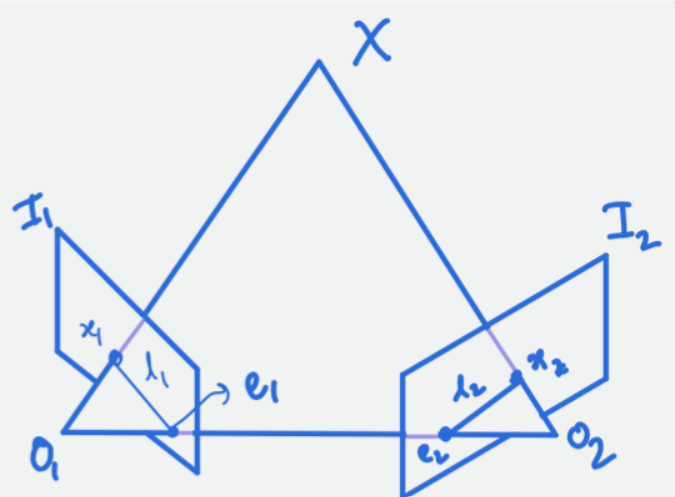
\includegraphics[width=12cm]{img/algebraic-fundamental.png}
    \caption{}
    \label{fig:Algebraic-fundamental}
\end{figure}

We will assume that the world coordinate system coincides with the camera coordinate system of our first image. Hence, we define:

\begin{equation*}
    O_1 = [I_{3\times3}|0_{3\times1}]
\end{equation*}

where this is the transformation between world coordinates to camera coordinates for frame 1. On the other hand, $O_2$ is the transformation to the second frame, which we will write relative to the first frame. That is, rotate and translate frame 1 to get frame 2. Hence,

\begin{equation*}
    O_2 = [R_{1\to 2}|t_{1\to 2}]
\end{equation*}

For simplicity, we will represent $R^2_1$ as rotation from 1st frame to 2nd frame.

Putting it all together, we have two set of equations:

\begin{equation}
\begin{split}
    &\lambda_1 \overrightarrow{p_1} = K[I|0]\overrightarrow{X}_{4\times1} \\
    &\lambda_1K^{-1}\overrightarrow{p_1} = \overrightarrow{X}
\end{split}
\end{equation}

Here, $K^{-1}\overrightarrow{p_1}$ is the normalized X coordinate $[X, Y, f]$ and $\lambda_1$ is the scaling factor. What is $\overrightarrow{p_1}$? This is the coordinate $[X, Y, 1]$ - the image coordinates.

The other equation is:

\begin{equation}
\begin{split}
    &O_2 = [R_{1}^2|t_{1}^2] \\
    &\lambda_2\overrightarrow{p_2} = K[R_1^2|t_1^2]\overrightarrow{X}\\ 
\end{split}
\end{equation}

Now, we know that $O_1O_2X$ forms the epipolar plane. Now, $O_1X$ is the same as $\lambda_1\overrightarrow{x_1}$. Now, we know that the dot product of two perpendicular lines is zero. Hence, we can write the following:

\begin{equation}
\begin{split}
    &\overrightarrow{O_1X}\cdot(\overrightarrow{O_1O_2} \times \overrightarrow{O_2X}) = 0 \\
    &\implies \lambda_1\overrightarrow{x_1}\cdot(\overrightarrow{t_1^2}\times R_2^1\lambda_2\overrightarrow{x_2}) = 0 \\
    &\implies \lambda_1\lambda_2\overrightarrow{x_1}(\overrightarrow{t_1^2}\times R_2^1\overrightarrow{x_2}) = 0\\
    &\implies \overrightarrow{x_1^T}[t_1^2]_{\times}R_2^1\overrightarrow{x_2} = 0 \\
    &\implies \overrightarrow{x_1^T}E_2^1\overrightarrow{x_2} = 0 \\
\end{split}
\end{equation}

Here, note that $\overrightarrow{O_1O_2}$ is represented by translation because that is in fact the transformation between the camera centers! Further, we are writing all these calculations in terms of frame 1. Hence, all coordinates have been transformed to the frame one relatives (by multiplying $R_2^1$ for instance). 

The matrix $E$ seen there is the \textbf{essential matrix} that relates points in terms of normalized pixel coordinates. $E$ has 5-6 degrees of freedom depending on the choice of looking at E - as a projective matrix or not (Wikipedia).

$F$ is something more - fundamental lol. 

\begin{equation}
\begin{split}
    &\implies  \overrightarrow{P_1}^TF_2^1\overrightarrow{P_2} = 0 \\
    &\text{ where $F_2^1 = K^{-T}[t_2^1]_{\times}R_2^1K^{-1}$}
\end{split}
\end{equation}

\subsection{Computation of $F$}

The fundamental matrix $F$ satisfies the equation $x'^TFx = 0$ and in order to calculate this matrix, we require at least 7 correspondence points (x maps to x'). 

* why there are 7 degrees of freedom *

I am lazy to write this part. Look at chapter 11 of the textbook for this section. 

\subsection{Normalized Eight Point Algorithm}



\subsection{RANSAC}

RANSAC isn't specific to multi-view geometry and can be used anywhere where there are outliers in our data. Now, with our data we will always have noise and we cannot choose any eight points and apply the eight point algorithm. RANSAC helps with this since outliers have little influence on the result. 

We will randomly take the minimum number of points required to determine the model parameters. Now, we can use the eight point algorithm and find the parameter. Then, determine how many points (from the set of all points) fit with the parameters chosen earlier. If the number of outliers are below a threshold, these parameters are acceptable. Repeat the same steps until the threshold has been met (if not met already obviously). 

The additional hyperparameters would be number of iterations, tolerance, etc. More about this can be read \href{http://www.cse.yorku.ca/~kosta/CompVis_Notes/ransac.pdf}{here}.

\section{Stereo Camera}

A stereo camera can be thought of as a special case of epipolar geometry - it is a combination of two monocular cameras separated by a fixed distance (lie on a common line called baseline). Now, if both cameras take an image and point to the same feature, we can find the world point.

Contrary to a monocular situation, with stereo cameras we know the exact distance between the cameras. 

\chapter{Triangulation and Perspective-n-Projection}

\section{Triangulation}

In epipolar geometry, we were never concerned with scene structure, we just wanted positions on images. Now, we will try to find the world point given two views or two images of a world point.

Let $x_1, x_2$ be the coordinates of the image in homogenous coordinates for camera 1 and camera 2. Now, there are rays from each camera center:

\begin{equation*}
\begin{split}
    r &= K_1^{-1}x_1 \\
    s &= R^1_2K_2^{-1}x_2 \text{ where $R^1_2$ converts to image one camera frame}
\end{split}
\end{equation*}

With epipolar geometry, we weren't able to determine the world point but we want to try approximating it - done with triangulation. 

Finding the point of intersection for two rays is easier said than done as due to errors in correspondence points, the rays may not intersect. Hence, an approximation will be minimizing the distance between two rays. Obviously, for intersection lines, the distance will be zero.

The points that give us the minimal distance will be such that the difference between two points is perpendicular to the direction of the ray.

Once we obtain the line segment that minimizes the distance, we will find the midpoint of this line and state that it is our estimate of the point in the triangulated world. 

\section{Perspective n Point}

Here, we are given 3D worldpoints and the 2D image correspondence in the camera frame. In simpler terms, the points on the image and the point for each feature in the real world is also known. With this information, we want to calculate the extrinsics of the camera. 

This concept is used extensively in augmented reality. We can see confirmation of this  \href{http://vr.cs.uiuc.edu/node292.html}{here (virtual reality, same concept)}

With P3P we are given 3 points and find the extrinsic parameters of the \textbf{calibrated} camera unlike in DLT. In DLT, we used an uncalibrated camera (also, 11 unknowns, so 6 points are needed). 



\chapter{Bundle Adjustment}

Usually, we have some noise in our measurements, either with our extrinsics or intrinsics. Hence, after triangulation, we will have some noise in our predictions. Refining the estimates is bundle adjustment. "Given a set of images depicting a number of 3D points from different viewpoints, bundle adjustment can be defined as the problem of simultaneously refining the 3D coordinates describing the scene geometry, the parameters of the relative motion, and the optical characteristics of the camera(s) employed to acquire the images, according to an optimality criterion involving the corresponding image projections of all points." from wikipedia.

Bundle adjustment is a non convex optimization problem that solves for camera parameters and 3D point locations of the environment. It takes the initial estimates of our camera estimates, 3D point locations, the image correspondences for the 3D point. By non convex, we mean that there are multiple local minimas as well. Hence, bundle adjustment only finds the local minima and assumes that the initial estimates are pretty good to begin with.

We are essentially minimizing the sum of squared errors after reprojecting the points over various images. This is generally expressed as:

\begin{equation}
    arg \min_{X_j, P_i} \sum_{i=1}^M\sum_{j=1}^N \norm{x_{ij} = P_iX_j}^2
\end{equation}

where $P_i$ is the projection matrix of the ith view, $x_{ij}$ is the image of the $jth$ 3D point in the ith view.

Look at the chapter on optimization in the SLAM section to see how we can solve such a problem - it involves using an iterative approach with gradients. This is a non-convex optimization problem so we can't find a closed form solution any way.

\part{State Estimation}

\chapter{Recursive State Estimation}

Let's assume that we are moving in an environment, we are tasked with estimating the environment and our position. We are doing something similar here as compared to multi view geometry, but recursively.

Let's say we have data upto a time $t$, and we wish to estimate the state of the system at $t+1$th instant. In most of the methods mentioned earlier, there was no time factor involved. Here, we want to use time series data to estimate the next belief state. Just as in dynamic programming, to estimate $t+2$th instant, we don't want to restart everything. In essence, we don't want to estimate the state of the system.

With recursive state estimation, we only use the new data that is incoming to estimate and do not use data till that time $t$. We assume that the information till that point has been incorporated already and we move from belief at time $t$ to belief at time $t+1$. This is very similar to the markov chain discussed in probability. This chapter will explore bayes filter, kalman filter and more. 

\section{Bayesian Filter}

Our goal is to estimate the state of the system $x$ given the observation $z$ and controls $u$. Imagine an environment filled with pillars, and as a robot moves we want to estimate the state of the system. Obviously this is important because we cannot control a robot without knowing where it is. The control is what command we give. The observation is our observation of where we are. This is very similar to the POMDP scenario where we have observations, actions and belief states. The observations can be derived from a sensor (laser range finder, GPS, etc). This can be concisely be represented as:

\begin{equation}
    bel(x_t) = P(x_t|z_{1:t},u_{1:t})
\end{equation}

Our goal is to represent this information using $x_{t-1}$.

\begin{figure}
    \centering
    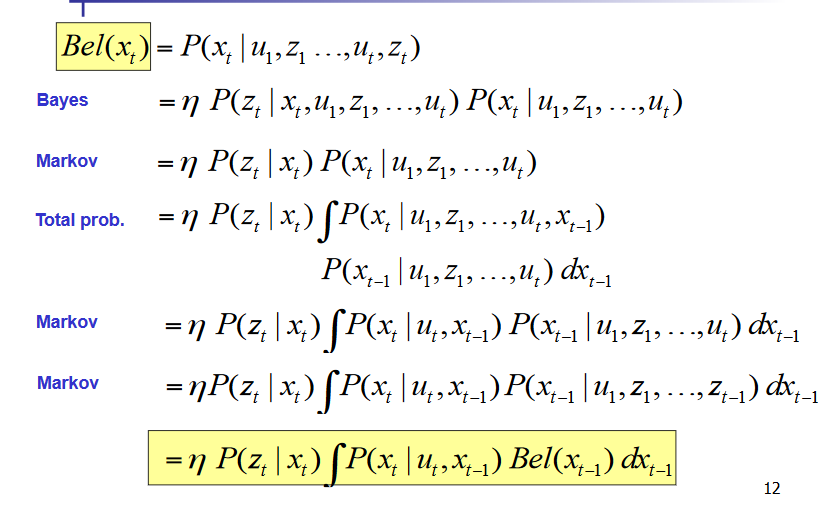
\includegraphics[width=8cm]{img/bayes-filter.png}
    \caption{Bayesian Filter Derivation}
    \label{fig:bayes_filter}
\end{figure}

\textbf{Markov Assumption}

The Markov assumption is that observation of the system at a time $t$ is only dependent on the time $t$ and not on any of the observation before it. Hence, we need not use $z_{1:t}$ and $u_{1:t}$ since we used that information already to arrive at our current state.

The bayesian filter is a framework for recursive state estimation.

\begin{equation}
    \hat{bel(x_t)} = \int p(x_t\|u_t, x_{t-1})bel(x_{t-1})dx_{t-1}
\end{equation}

After correction, we get:

\begin{equation}
    bel(x_t) = \eta p(z_t\|x_t)\hat{bel(x_t)}
\end{equation}

\section{Kalman Filter}

This is essentially a bayesian filter with gaussians - a very popular filter. We know what a gaussian is already. For a multivariate gaussian, it looks something like:

\begin{equation}
    p(x) = \frac{1}{(2\pi)^{d/2}\abs{\Sigma}^{1/2}}e^{-\frac{1}{2}(x-\mu)^t\Sigma^{-1}(x-\mu)}
\end{equation}

\begin{figure}
    \centering
    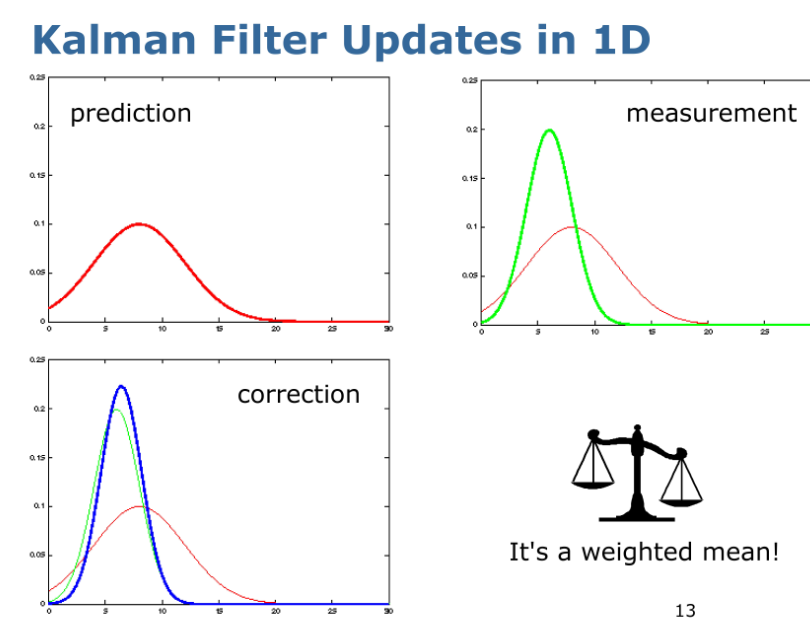
\includegraphics{img/kalman.png}
    \caption{Kalman Filter}
    \label{fig:kalman}
\end{figure}

He didn't really cover this in much detail but it uses covariance matrices and a concept called "Kalman" gain to make updates to the estimate.

\section{Extended Kalman Filters}

So far, we've only looked at linear functions. Kalman filters work with gaussian distributions and linear functions. But the world isn't that \textbf{straight} forward (badum-tus). Non linear functions needn't preserve the initial distribution and the kalman filter can BREAK. 

So, we find a hack and try to linearize our non-linear functions. This is usually done with a Taylor series expansion. For higher dimension data, note that we use jacobians to linearize the data.

\part{SLAM}

\chapter{Optimization}

Before looking at SLAM, it's important to look at some fundamental math that is used. These techniques aren't limited to SLAM and have other uses, and the next chapter may not even mention these methods but these are relevant nonetheless. 

\section{Convex Optimization}

Convex optimization is a special class of problems that deals with convex problems. There is a popular book by Stephen Boyd - \href{http://93.174.95.29/main/B8624D493F5332A34A826B9CC74B88B1}{Convex Optimization} (the link is a ps.gz file). 

In general, an optimization problem is one where you minimize a function set to certain constraints. A lot of problems can be posed as an optimization problem. Redundant to explore what it means to optimize in more detail since we've already seen instances in the math review section. 

\section{Linear Least Squared Optimization}

In the end, problems such as SLAM have a common goal - minimize a function. Often, these problems are posed as least squares systems.

\begin{equation}
\begin{split}
    &Ax=b \\
    &A\text{ is }m\times n \text{ matrix where } m > n
\end{split}
\end{equation}

For this chapter we consider overdetermined systems (more data than required) and full rank (due to noise). It is full rank because the rank of the matrix is the column rank ($n < m$) and all columns are linearly independent. We can say that the columns are linearly independent because of the noise in the data.

As per Boyd:

A least-sqaures problem is an optimization problem with no constraints and an objective which is sum of squares of the form $a_i^Tx-b_i$:

\begin{align}
    \text{minimize }f_0(x)=\norm{Ax-b}_2^2 = \sum_{i=1}^k(a_i^Tx-b_i)^2
\end{align}

We've encountered this formulation before as well while doing linear regression. The solution can be reduced to solving this equation:

\begin{equation}
    (A^TA)x=A^Tb
\end{equation}

and the analytical solution would be:

\begin{equation}
    x=(A^TA)^{-1}A^Tb
\end{equation}

The time taken to solve this problem varies depending on the sparsity of the matrix $A$. Sparsity refers to the number of non-zero entries in the matrix.

\subsection{Norm Approximation}

The simplest norm approximation problem is an unconstrained problem of the form

\begin{equation}
    \text{minimze } \norm{Ax-b}
\end{equation}

We can pose this as a least squares approximation by squaring the l2 norm. This would be:

\begin{equation}
        \text{minimze } \norm{Ax-b}_2^2
\end{equation}

The analytical solution to this problem can be solved by using this convex quadratic function:

\begin{equation}
    f(x) = x^TA^TAx - 2b^TAx + b^Tb
\end{equation}

A point $x$ minimizes $f$ iff the derivative is 0:

\begin{equation}
    \nabla f(x) = 2A^TAx - 2A^Tb = 0
\end{equation}

This is the same formulation that we had earlier and will yield the solution $x=(A^TA)^{-1}A^Tb$.

\textbf{How do we know that $A^TA$ is invertible?}

The assumption here is that the columns of $A$ are linearly independent. In that case, let $x$ be a vector that satisfies $(A^TA)x=0$. Multiplying by $x^T$ on both sides,

\begin{equation*}
    0 = x^T0=x^T(A^TA)x=x^TA^TAx=\norm{Ax}^2
\end{equation*}

So, $Ax=0$ and columns of A are linearly independent. Hence, the only solution to this is $x=0$. This is also the only solution to $A^TAx=0$, which means that $A^TA$ is invertible. 

\textit{Why is that last sentence true?}

If $x=0$ is the \textbf{only} solution to the equation $Ax=0$, then this is case. Or, the nullspace of $A$ is limited to zero vector if and only if $x=0$ is the only solution to $Ax=0$. 

In a singular matrix, the matrix does not have an inverse and the nullspace will have more than the zero vector. - this part is obvious but wasn't immediately clear at the time.

Here the pseduoinverse is $A^\dagger = (A^TA)^{-1}A^T$. The pseudoinverse takes on various forms depending on the type of system - overdetermined, undertermined, and full row, full column rank cases. Information about these cases can be found \href{https://math.stackexchange.com/questions/1537880/what-forms-does-the-moore-penrose-inverse-take-under-systems-with-full-rank-ful/2200203#2200203}{in this stack overflow answer}. The logic behind the SVD decompositions and the "proofs" aren't very explanatory though.

\subsection{Using SVD}

This algorithm is from the appendix of MVG by Ziesserman:

\begin{enumerate}
    \item Find the SVD $A=UDV^T$
    \item Set $b'=U^Tb$
    \item Find the vector $y$ defined by $y_i = b_i'/d_i$ where $d_i$ is the $i-$th diagonal entry of $D$
    \item The solution is $Vy$
\end{enumerate}

\section{Non-Linear Optimization}

Nonlinear optimization is the term used to describe an optimization problem when the objective or constrain functions aren't linear and not convex. As a result, these non linear problems are particularly hard for even low number of variables.

These sections are largely from Boyd's book on 'Convex Optimization'.

\subsection{Local Optimization}

Local Optimization is akin to solving for a local minima. With a non-linear function, the search space can be unbelievably large and difficult to navigate. As such, it is more convenient and computationally feasible to search for the best value within a certain range. We may not get the best solution but may get a "good solution". This is familiar because it was explored earlier with gradient descent - we may hit a local minima. 

The trick with this is that local optimization will tend to be iterative and most importantly, rely on a good initialization. This reminds of the genetic algorithm assignment in MDL - depending on where you start your search space, you are restricted to the best values in that area.

\subsection{Global Optimization}

The task with global optimization is the BEST point for our formulation. This is an extremely difficult challenging problem and the compromise here is effeciency of computing the solution. The worst case complexity of global optimization tends to grow exponentially with increasing complexity. This is useful for cases where we NEED to find the absolute maxima or a minima in situations such as safety. We need to be assured that the worst case scenario can still be handled for instance, in which case we are dealing with a global optimization problem for the global worst point.

\section{Unconstrained Minimization}

Often, even for convex problems, it is not possible to arrive at an analytical solution by setting the derivative to zero. There may be multiple reasons for this - yet to see a reason for this but Boyd says so. Hence, we rely on an iterative algorithm to solve the optimality equation.

\subsection{Gradient Descent}

This has already been explored but anyway. Here, we move in the opposite direction of the gradient. The gradient is the direction of steepest ascent. 

\begin{equation}
    \Delta x = -\nabla f(x) = -J_f
\end{equation}

\subsection{Newton's Method}

Here, the step is defined as:

\begin{equation}
    \Delta x = -\nabla^2[f(x)]^{-1}\nabla f(x)
\end{equation}

This is like the gradient descent but just that we use the newton step defined above as the search direction. Newton's method is known to provide faster convergence for optimization (more positive reasons in Boyd) but is not commonly used. This is primarily because of the cost of forming and storing the hessian, and the cost of computing the newton step.

\section{Non-Linear Least Squares}

This problem involves solving a least square formulation of a non linear function.

\begin{equation}
    \text{minimize }\norm{f(x)}^2
\end{equation}

To accomplish this, we can do this:

\begin{equation}
    \text{minimize }F(x) = \frac{1}{2}f(x)^Tf(x)
\end{equation}

\textit{We add the 1/2 term because it makes the derivative better - it doesn't change the function optima obviously.}

\subsection{Gauss-Newton}

The Gauss-Newton algorithm can be used to solve non-linear least-squares problems. It essentially solves for the function mentioned above.

Here, the update rule is:

\begin{equation}
    \Delta x = -(J^TJ)^{-1}J^Tf(x)
\end{equation}

It tries to model the curvature of a region.

\subsection{Levenberg Marquardt}

"The Levenberg-Marquardt algorithm combines two  minimization methods: the  gradient descent method and the Gauss-Newton method.  In the gradient descent method, the sum of the squared errors is reduced by updating the parameters in the steepest-descent direction.  In the Gauss-Newton method, the sum of the squared errors is reduced by assuming the least squares function is locally quadratic, and finding the minimum of the  quadratic.   The  Levenberg-Marquardt  method  acts  more  like  a  gradient-descent method  when  the  parameters  are  far  from  their  optimal  value,  and  acts  more  like the Gauss-Newton method when the parameters are close to their optimal value." from \href{http://people.duke.edu/~hpgavin/ce281/lm.pdf}{Duke Notes}.

\begin{equation}
    \Delta x = -(J^TJ + \lambda I)^{-1}J^Tf(x)
\end{equation}

\href{https://cs.nyu.edu/~roweis/notes/lm.pdf}{These notes} give a good description about ideal step sizes. In short, when we are at a steep cliff, we want to take small steps to avoid overshooting, and when we are at a gentle slope, we want to take bigger steps because who has time to tip-toe. This method aims to solve that by being a blend of SGD and Gauss-Newton parameterized by a variable $\lambda$ (blending factor) that determines how much closer we are to SGD or Gauss-Newton. 



\chapter{SLAM Pipeline}

If we consider mobile robotics to be comprised of: "Where am I", "Where am I going", and "How do I get there", SLAM answers the first (Leonard and Durrant Whyte). So, what is SLAM? A robot observes the environment relative to its unknown pose, this helps localise the position. On the other hand, if we know our location, we can create a map of the environment based on the sensor inputs we have. Hence, the simultaneous localization and mapping. 

I really really liked \href{http://www.informatik.uni-bremen.de/agebv2/downloads/published/freseki10.pdf}{this paper that explains SLAM from a user perspective}. It abstracts the math away for a while, to focus on the bigger picture.

"The  need  to  use  a  map  of  the  environment  is  twofold. First,  the  map is  often  required  to  support  other  tasks;  for instance,  a  map  can  inform  path  planning  or  provide  an intuitive visualization for a human operator. Second, the map allows limiting the error committed in estimating the state of the  robot.  In  the  absence  of  a  map,  dead-reckoning  would quickly drift over time; on the other hand, using a map, e.g.,a  set  of  distinguishable  landmarks,  the  robot  can  “reset”  its localization  error  by  re-visiting  known  areas  (so-called loop closure). Therefore, SLAM finds applications in all scenarios in which a prior map is not available and needs to be built." from \href{https://arxiv.org/pdf/1606.05830.pdf#page=1&zoom=auto,-18,801}{ a review paper}

\section{The Big Picture \& State of the Art}

First, based on data received by the sensors we will extract features. These features are then passed to a data association block which tracks features (short term) and loop closure (long term with bag of visual words). Feature tracking is essentially feature matching (optical flow) between two close frames. Visual odometry is then done after feature tracking to calculate the transformations between robot poses. If we have sensors like wheel odometry, we can also do EKF fusion - gives us a better estimate of wheel odometry. There are some packages which also perform local bundle adjustment. The output of the frontend is keyframe poses and loop closure pairs which feeds into the backend.

The backend will then optimize the results given by frontend and obtain optical relative transformation. The global map is then assembled based on optimized poses and local point clouds.

As per the review paper mentioned earlier, the frontend is where SLAM meets other research fields - computer vision and signal processing, the backend is more mathematical and involves optimizations, and probabilistic estimation.

One key thing to note when looking at the loop closure section is that it makes SLAM unique. Otherwise, this is just an odometry problem. 

\section{Iterative Closest Points}

Let's say that we have a vehicle which is moving and constantly taking pictures of the world around it. It has some features or point clouds with respect to the frames at two different instances. Now, if we want to figure out the transformation between these two frames, how do we go about it? ICP is the task of finding parameters of the transformation that best aligns corresponding data points. Or estimating our state using point set registration. We usually solve this as an optimization problem, where we have two sets of points, and a hypothetical transformation between them. So with a series of equations, we can solve for a solution.

\begin{figure}
    \centering
    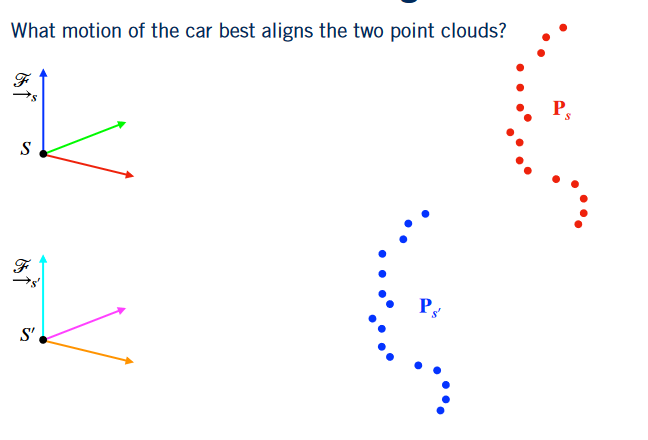
\includegraphics[width=8cm]{img/icp.png}
    \caption{Illustration of point registration for state estimation task}
    \label{fig:state_estimate}
\end{figure}

Now, we have some problems - we don't always know which points correspond to another from our two sets of points. So, if we assume that our transformation was very tiny, we can reduce the possibilities of what point corresponds to another. We can then set an initial GUESS for the transformation - an identity transform and then work with this to find the ideal transform. The intuition is when the optimal motion is found, corresponding points will be closer to each other than to other points. For small displacements, this heuristic works: For each point, the best candidate for a corresponding point is the point that is closest to it right now.

\textbf{Procedure:}

\begin{itemize}
    \item Get an initial guess for the transform $\{R^{s'}_{s}, t\}$
    \item Associate each point with a corresponding one.
    \item Solve for optimal transformation
    \item Repeat till convergence
\end{itemize}

The key thing here is the knowledge of corresponding points is important. Sometimes it is known, sometimes not. In the former case, we have to directly aim for a solution, but in the latter we work on first estimating some correspondences and then looking for a transform (like the algo above). This guesstimate can be found by drawing a normal from a point and seeing what corresponding point we hit. This iterative algorithm is ICP. Look at \href{https://www.notion.so/Point-Cloud-Registration-Iterative-Closest-Point-a25686ce1a11409d838d47bcac43ab4b}{Shubodh's notes from Mobile Robotics} for more explanation about ICP.

\href{https://igl.ethz.ch/projects/ARAP/svd\_rot.pdf}{This resource} on least square ICP solution using SVD not only shows how to solve it (section 4), but offers a detailed proof on how to go about things. The stachniss lectures don't go into detail about WHY we use this as a solution. \textit{It's so well written gahhhhh.}

As mentioned earlier, there are two things:

\textbf{Known correspondences}

Here, we have the luxury of posing this as an equation that must be solved. If we assume that our points are $\{p_i\}$ and $\{q_j\}$, then we can find the centroid (or mean of points) of each of these sets. We can safely state that the transformation between these points is the same that the centroid will undergo.

We then do a singular value decomposition. The solution for the problem then becomes $UV^T$. Page 10 of \href{https://arxiv.org/pdf/1705.09785.pdf}{this paper by MK} has a real clear explanation on why that is. As mentioned earlier, the translation between centroids is equivalent to the translation between ALIGNED frames. This information lets us solve for just the rotation matrix.

\textbf{Unknown correspondences}

If the correct correspondences are not known, it is generally impossible to determine the optimal relative rotation and translation in one step. The algorithm converges if starting positions are “close enough”. There are various matching algorithms, some of which are shown \href{https://www.notion.so/Point-Cloud-Registration-Iterative-Closest-Point-a25686ce1a11409d838d47bcac43ab4b#acdbf05aa6834446bc0812b2ae3f0f40}{here} - Closest-point, normal shooting, etc. This data association has a very high impact on convergence and speed.

It is possible to use feature extractors and have feature correspondences as well. But this is easier said than done since we will be dealing with LiDAR data often for point clouds.

Some variants of ICP can be seen in Shubodh's notes. 

\subsection{Solving ICP}

We tend to consider overdetermined systems here, we have $m\geq n$. We are solving for something like $Ax=b$ where $A$ is a full rank matrix (rank = $\min (m, n)$. There are a lot of ways to solve for this regularly but for the purpose of discussion, we will try to find the optimal $A$. This matrix just needs to get most of the transformations right, so we pose it as a least squares chapter as seen in the last chapter (and can solve in that way as well).

In ICP, we are solving for 6 variables. Each point gives rise to 3 equations, so with two points we can technically solve for it. But our point cloud is more dense than that, so we end up with an overdetermined solution. 

A SVD solution to ICP has already been shown in that earlier paper by MK.

\subsubsection{ICP as Least Squares}

Let's assume that we have a set of m points in frame I, J - $\{P_i\}$, $\{Q_j\}$.

\begin{equation}
    \Vec{P_i} = R\Vec{Q_i} + t
\end{equation}

We can represent the R matrix using Z-Y-X euler angles for ease. But this has non-linear terms - many $\cos$ and $\sin$. So, for ease, we make a small angle assumption (like before) because of which, we can say that:

\textit{He mentions that we could have linearised instead by taking the Jacobian. And, using Taylor approximation leads to small angle assumption.}

$\cos \alpha = 1$, $\sin \alpha = \alpha$ and so on. So, the resulting rotation matrix becomes:

\begin{equation}
\begin{bmatrix}
1 & -\alpha & \beta \\
\alpha & 1 & -\gamma \\
-\beta & -\gamma & 1\\
\end{bmatrix}
\end{equation}

Hence, we can rewrite our transformation between frames as :

\begin{equation}
\begin{bmatrix}
1 & -\alpha & \beta \\
\alpha & 1 & -\gamma \\
-\beta & -\gamma & 1\\
\end{bmatrix} \begin{bmatrix}Q_{x_1} \\ Q_{y_1} \\ Q_{z_1}\end{bmatrix} + \begin{bmatrix}t_x \\ t_y \\ t_z\end{bmatrix} = \begin{bmatrix} P_{x_1} \\ P_{y_1} \\ P_{z_1} \end{bmatrix}
\end{equation}

\textit{t is the translation of Q wrt P}

Now, we can easily write this in the form of $Ax=b$. This ends up becoming:

\begin{equation}
    \begin{bmatrix}
    -Q_{y_1} & Q_{z_1} & 0 & 1 & 0 & 0 \\
    Q_{x_1} & 0 & -Q_{z_1} & 0 & 1 & 0 \\
    0 & - Q_{x_1} & Q_{y_1} & 0 & 0 & 1 \\
    \end{bmatrix} \begin{bmatrix}
    \alpha \\
    \beta \\
    \gamma \\
    t_x \\
    t_y \\
    t_z \\
    \end{bmatrix} = \begin{bmatrix}
    P_{x_1} - Q_{x_1} \\
    P_{y_1} - Q_{y_1} \\
    P_{z_1} - Q_{z_1} \\
    \end{bmatrix}
\end{equation}

This is just for one correspondence, so we can stack each correpsondence such that we get:

\begin{equation}
    \begin{bmatrix}
    A^1 \\
    A^2 \\
    \vdots \\
    A^m
    \end{bmatrix} X = \begin{bmatrix}
    b^1 \\
    b^2 \\
    \vdots \\
    b^m
    \end{bmatrix}
\end{equation}

\textit{Why are we doing n points again? Because some correspondences may be wrong, so we want more data points.}

Check the last chapter to see how SVD can be used to solve least squares problems. There are various ways to go about solving ICP.

BUT, there is a problem here - we had to make a small angle assumption. Let's express this problem in a new way now:

\begin{equation*}
    Ax = b
\end{equation*}

\begin{equation}
    \begin{bmatrix}Q_{x_1} & Q_{y_1} & Q_{z_1} & 000 & 0 & 0 & 0 & 1 & 0 & 0 \\
    \hdots \\
    \hdots \\
    \end{bmatrix} \begin{bmatrix}r \\ \vdots \\ t\end{bmatrix} = \begin{bmatrix}P_{x_1} \\ P_{y_1} \\ P_{z_1}\end{bmatrix}
\end{equation}

The above equation essentially stretches the rotation matrix, and stacks it on top of the translation vector. We are able to write $P = RQ + t$ in this form as a result. 

Now, why can't we use this to solve as a least squares problem. We just have more variables - 12 here (the rotation, translation vector). The variables aren't independent! There are many constraints that come with the values being a part of rotation matrix. These constraints are $RR^T=I$, $\norm{R_i}=1$. These constraints make the solution a non-convex one (ref prev chapter for explanation). This is a manifold optimization problem, consider a locally euclidian space, take it to a tangential space and work there and return to eulician space. Note that rotation matrices aren't euclidian (you cant add rotations to combine rotations for instance). 

In principle, we can linearize the equation above, and use the Jacobian to write it using Taylor series. 

\textit{We always made a full rank assumption here (which holds true because of noise as discussed in some other chapter), but this can fail if the points are coplanar or colinear (depends on the situation).}

\subsection{Multiview ICP}

How to get the right poses AND the map from noisy estimates of poses and the map? 

$T_0 = \begin{bmatrix}I & 0 \\ 0 & 1\end{bmatrix}$ is the origin. We are generally using homogenous equations. Here, the rotation is identity, indicating that we are at origin (translation is origin too). 

The robot has move, its estimating position, and estimating point clouds but it makes errors!

We will pose ICP as a multiview optimization to alleviate the error.

The insight: If there is a grame $\{q\}$ in which the depth measurements and the point cloud $\hat{X_{qj}}, j=\{1,\hdots,n\}$ are particularly noiseless. Can this be used to alleviate other views in terms of poses and 3D pooints estimated in those views. 

If a set of n points are viewed in m frames or observations what is the best estimate for these n points and m poses. - Multiview aggregation and Multiview consistency.

\section{Loop Closures}

\href{https://www.notion.so/Loop-Closure-8ab30a4560ea4d859c92c515c99ef70a}{Summer school loop closure notes} can be found here - Udit made them.

\begin{figure}[h]
    \centering
    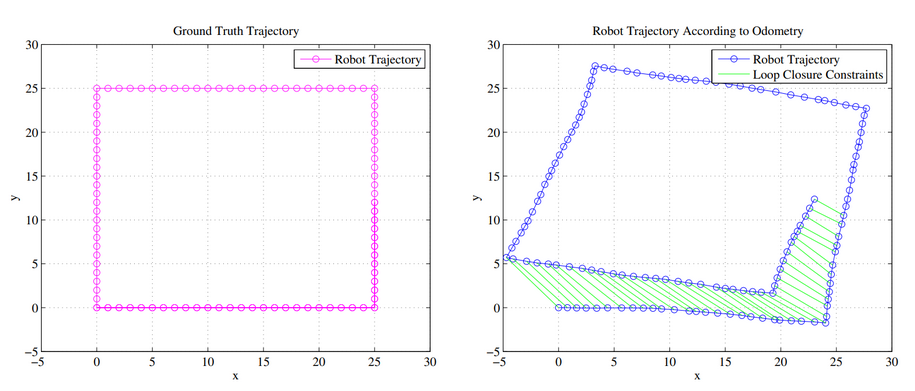
\includegraphics[width=12cm ]{img/loop_closure.png}
    \caption{Loop Closure}
    \label{fig:loop_closure}
\end{figure}

Information that is fed into SLAM is relative to the position of the robot. So, as we move along, the predictions we make are dependent on the previous positions. As a result, errors can accumulate over time causing problems. In contrast to this, the shape of the room is fixed and won't change. 

Now, assume that the robot moves along a closed loop, returns to the start of the loop but it may not know this yet.  Look at the image above, it shows the actual trajectory of the robot. But, using odometry measurements, it predicts the positions on the right. Loop closure works to enforce constraints on the mapping between points that are revisited. This is a challenging problem because it has to detect same locations (data-association again gargh).

If we consider SLAM as a conditionaly dependency graph - visualize this as a set of nodes over time, now after moving, some nodes will be repeated. Loop closure helps ensure that the two repeated nodes similar.

A  robot  performing  odometry  and  neglecting  loop closures interprets the world as an “infinite corridor”. Look at page 2 of \href{https://arxiv.org/pdf/1606.05830.pdf#page=3&zoom=110,106,607}{this review paper} to see why Loop closure is important in more detail.

On the note of data association, one technique that is used is Bag of Visual Words

\subsection{Bag of Visual Words}

Imagine that you have some important tasks such as finding images with a theme or text with some tags. This is a hard task where linearly searching for similarity isn't feasible. The solution is to extract some good features and construct a set of them, and construct a histogram based on the occcurences of these features. Now, using this lower dimension representation of our data, we can perform our operations sooner.

So, we extract feature descriptors from SIFT/ORB, cluster using K-Means to get final visual words in a dictionary. The centroids form the required dictionary.

We can use these histograms to compare our locations. This is often done using cosine similarity (another measure of distance) = $\frac{x^Ty}{\norm{x}\norm{y}}$.

As always, we want words that have high variance - if everything has something in common, why does it help us? 

\section{Review of Visual Odometry}

Motion estimation is called visual odometry - estimating our poses given corresponding images. This can be done using 2D-2D, 3D-3D and even 2D-3D methods.

Considering the overwhelming number of algorithms mentioned so far, a quick review:

\begin{itemize}
    \item 2D-2D: Epipolar Geometry via Fundamental Matrix
    \item 3D-2D: Compute the 3d point given position of points in images and camera matrices
    \item 3D-2D: Given 3D points in world frame and 2D correspondences in camera frame, estimate camera motion/pose.
    \item 3D-3D: ICP
\end{itemize}

\section{Frontend}

\begin{figure}[h]
    \centering
    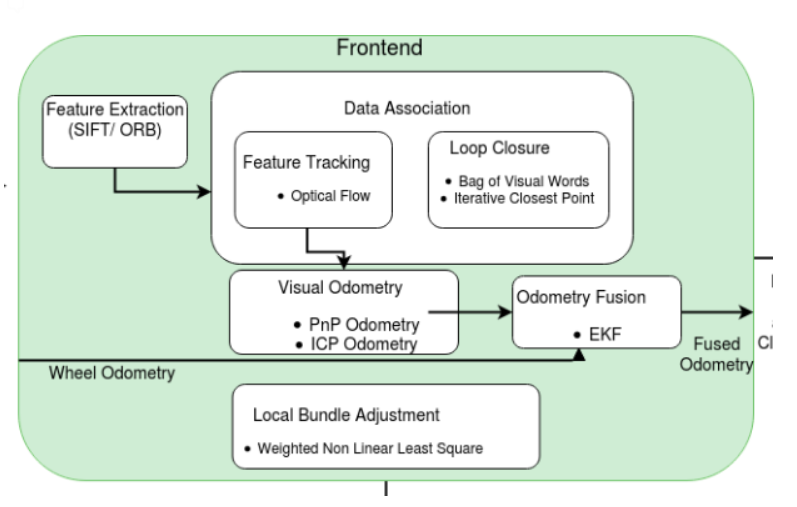
\includegraphics[width=12cm]{img/frontend.png}
    \caption{Frontend}
    \label{fig:frontend}
\end{figure}

The SLAM frontend detects features, matches them, and estimates motion using one of the algorithms mentioned above. Feature extraction can happen using something like SIFT. In the context of SLAM, good features are those that remain stable after camera motion. Harris corner is bad here cause it won't work well. We need points that are repeatable, distinct in representation, or local. ORB happens to be very fast. There are some direct methods for SLAM as well, seen \href{https://www.notion.so/SLAM-Frontend-Visual-Odometry-bd7dbccb797f442f955f450044ee200f#5346a971d36a4ac386c772228c7fe3bd}{here in Shubodh's notes.}

We can use Kalman filters to fuse multiple sensor streams.

\section{Backend}

\begin{figure}[h]
    \centering
    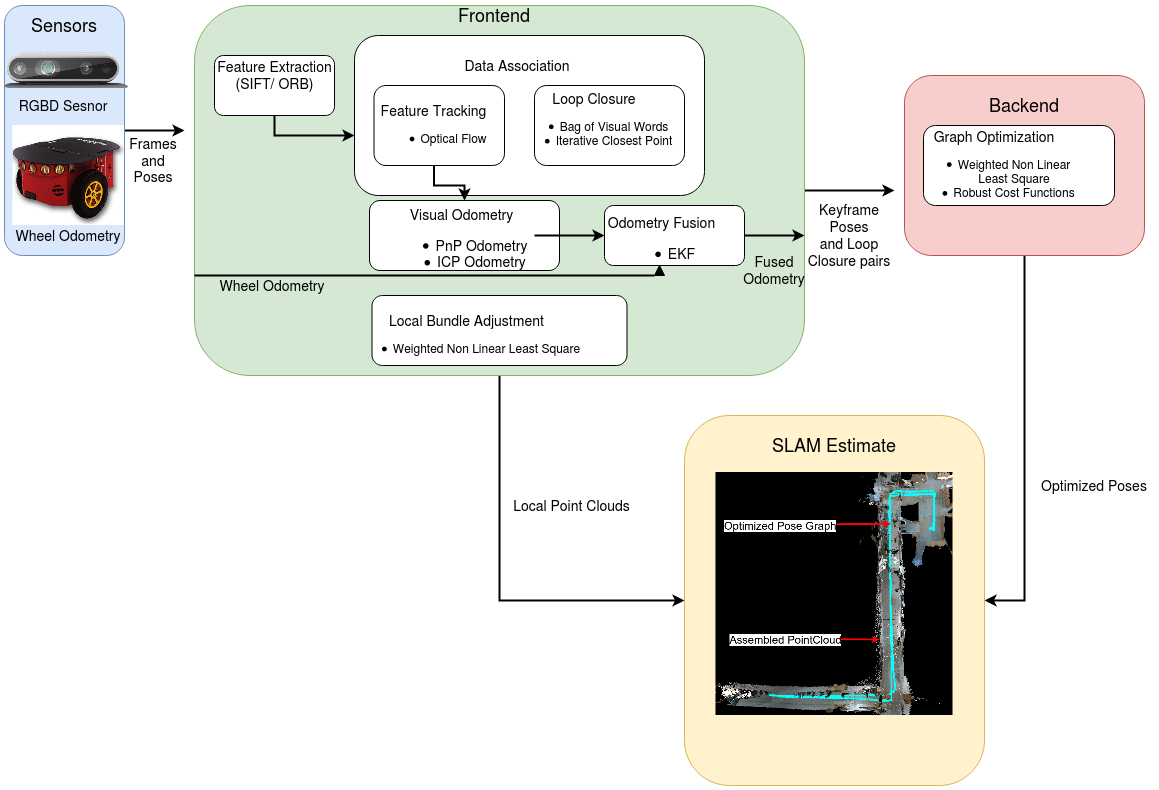
\includegraphics[width=12cm]{img/backend.png}
    \caption{Full Picture}
    \label{fig:slam}
\end{figure}

Now that we've seen the broad picture, we can see how various components will interact with each other. The SLAM Backend provides an interface to graph construction and optimization tools. It essentially forms the map of our SLAM system and uses pose estimates from the visual odometry to form the nodes of a graph. It also corrects drift in the VO estimates when the Place Recognition node flags a match between views. There's a lot math here and various approaches - using Bundle Adjustment or Pose Graph estimation.

\section{State of the Art and Applications}

SLAM has a wide range of applications in the mapping domain - \href{http://www.informatik.uni-bremen.de/agebv2/downloads/published/freseki10.pdf}{as shown well in this paper}. In augmented reality, where graphics are put on top of a camera image, we need to know the cameras position in the world. \href{https://sci-hub.tw/10.1109/ISMAR.2007.4538852}{The introduction to this paper on AR} has some insights into the application of SLAM for AR.

\subsection*{MonoSLAM}

MonoSLAM was the first ever monocular SLAM system. The frontend was very sparse feature point tracking. The backend was primarily done using Kalman filter. Given previous state of the camera and current landmarks, it would give the current state of the camera. 

\subsection*{ORD-SLAM}

This uses ORB feature extractor to get features. The entire system is calculated around ORB features including visual odometry and ORB dictionaries for loop detection.

\subsection*{Semi-Direct Visual Odometry}

This is a combination of keypoints (not descriptors) and information around the keypoints using direct methods. Direct methods tend to use the entire image. Just as the name suggests, it is not a complete SLAM pipeline. If there are some errors in odometry, the errors will propogate since there is no backend optimization here or loop closures here.

\subsection*{RTAB-Map}

RTABMAP is a classic solution in the RGB-D SLAM. It implements feature-based visual odometry, bag-of-words-based loop detection, back-end pose map optimization, and point cloud and triangular mesh maps. 

Support for multi-session mapping is provided, which allows the SLAM approach to initialize a new map with its own referential on startup, and when a previously visited location is encountered, a transformation between the two maps can be computed. This can be seen as a fancier version of loop closure as using ICP or so, we can combine maps that were separately made.

\subsection*{Semantic SLAM \& Future}

Till now, we've only explored SLAM that localizes and maps. Semantic SLAM will also classify items in the map giving the SLAM three layers - localization, mapping, and classification.

In 3D dynamic scene graphs, there are multiple layers to the SLAM - metric semantic mesh, objects and agents, places and structures, rooms, and buildings.

As per Andrew Davidson, there is robust localization, dense mapping and semantic understanding of the world. 

It can be said that semantic helps SLAM and SLAM helps semantics. Why?

So far, we've looked at static SLAM but when the environment is dynamic - the algorithms are bound to fail. With semantics, we may segment out humans and other dynamic objects. These semantics are critical to understanding the environment obviously - just as we are aware of moving objects in life. 

Now, typically in deep learning we have a series of images that aren't explicitly related. But with SLAM information, we can warp images to obtain new images (similar to ones that are seen) and we needn't make another forward pass.

\part{Motion Planning}

\chapter{Motion Planning}

In an autonomous vehicle, there is a decision making heirarchy. First, route planning then behavioural decision making (navigating through the route - making decisions about this such as traffic rules), which then determines motion planning which in turn creates trajectories for the vehicle to follow.

\begin{itemize}
    \item Route Planning
    \item Behavioral Decision Making
    \item Motion Planning
    \item Vehicle Control
\end{itemize}

There are two functions used in graph algorithms that are critical:

$g(n)$ = It is the cost of reaching the current node n from the start node
$h(n)$ = It is a heuristic function that gives us an estimate of the cost of reaching the end node from the current node n.
$h(n) \leq h*(n)$, 
Here, h*(n) is the actual cost of reaching the end node from the current node n.

For all search functions we will be storing the nodes in a priority queue Q which will be sorted in the increasing order of f(n) for each node.
$f(n) = g(n) + h(n)$

\section{Basic Algo for Search}

\begin{itemize}
    \item Initialize empty priority queue
    \item current node = start function 
    \item For every adjacent node, calculate respective f values and insert into queue.
    \item Once adjacent nodes are visited, mark as done (BFS)
    \item From queue, pick min f value and use as current node. If this isn't the target goal, repeat process from 3. again.
\end{itemize}

The above is essentially BFS. BFS gives us the shortest path between two nodes - but it needn't be the best path - traffic or bad roads?

\section{A* search algorithm}

It is a directed search algorithm, meaning instead of searching in all directions we search in the direction of the goal thus reducing the search time.

Here for every node, we calculate g(n) and h(n). If h(n) > h*(n), we might not end up with the optimal path to the goal.

The priority queue is sorted in increasing order of the f-values of the nodes.

This gives us the most optimal path to the goal in a short time.

\section{Rapidly Exploring Random Trees}

Often, we are not given a tree/graph with various nodes and hence cannot use graph methods. Hence, we will use rapidly exploring random trees. 

The idea is simple - start with just the start node. Now, create a node at a random point in the configuration space. If the random node does not lie inside any obstacle, we find a node in the graph which is closest to this node. If the distance between them is <= delta we connect them with an edge. If > delta we create another node along the line connecting the two nodes at a distance delta from the nearest node on the graph. We connect these two nodes with an edge and finally push this node inside the graph. This is repeated until we reach the goal location.

Let's assume that we have a set of global points which depict our path to a location. We are required to try sticking to these and the reference trajectory. Motion planning to this end, is mainly control. 

\section{Trajectory Generation}

Most of this content comes \href{https://raw.githubusercontent.com/RoboticsIIITH/summer-sessions-2020/master/lecture-slides/motion_planning/presentation.pdf}{these slides.}

There are two categories of robots broadly - non-holonomic and holonomic. Holonomic robots have the advantage of moving in any specific direction (like a drone) but non-holonomic (like cars) can't. A robotic arm is also non-holonomic since it is limited to a certain length.

We will tend to use with non-holonomic robots which are largely harder to use than holonomic. A drone has complete freedom to rapidly change directions, but a car would need to go in a circle to take a U turn for instance. Hence, with non-holonomic robots, we cannot rely on immediate configurations to move but rather have an entire trajectory to plan the movement. 

Often we'll have user requirements such as velocity, time to cover a distance and so on. So, here we will consider a 2D configuration space which is static in nature.

\subsection{Collision Avoidance}

This uses the idea of circles around the agents. If we predict that two agents are going to have "overalpping circles", it suggests a potential collision. Once again, a lot of math that I didnt understand - revisit later.

\section{Optimal Control}

Like any optimization problem, here too we are trying to minimize a cost function that has some constraints to it. We can choose to model it using a lagrangian for instance.

% \part{Dynamics and Drones}

% \chapter{Quadropter Dynamics}

\textbf{Why mathematical model}

It is a concise representation of the physical world that we can use to conduct prediction and analysis. 

\section{Kinematics v/s Dynamics}

In school, we tended to use these terms interchangeably. But, kinematics is the study of motion without considering the cause of motion. Dynamics looks at the force and moments in its study of motion.

\section{Rotation in free space}

Rotation happens at the center of gravity - the principle of least action. In fact, equations of motion happen with respect to center of gravity.

The drones exert two forces - thrust and the moment. The thrust from the blade rotations pushes it up. The moment is the "clockwise" / "anti-clockwise" direction that the drone can move in. Just as pushing in a certain direction on a rotating chair lets us rotate, blade rotations will rotate the drone. Drones do not rotate in real life like this because moments call each other.

There are three movements that the drone can do - roll, pitch, yaw. These are accomplished by varying the drone blade speeds such that the moments do not cancel each other out.

The standard for referencing the motors of drone follow an $\alpha$ pattern.

\chapter{Controllers}

When we have a system, we can imagine that it has various actuators. These actuators need some input to determine the change of the system in its environment. The controller then 

\section{On/Off Controller}

This is the most basic controller - it can perform only two actions and based on a threshold it will execute either. Hence, there are abrupt changes and for instance, the acceleration of a car with such a controller would change based on the location. This is clearly not practical since it is so abrupt.

The wave for this can be imagined as a square wave with time - fixed values only.

\section{P Controller}

Here we are setting the control proportional to the current state than switching between binary states. Hence, the frequency of oscillation reduces significantly. Still, the oscillation is dependent on distance from the initial state alone. So, in a car it will ignore velocity and only control acceleration of the car based on distance. The next controller solves this.

\section{PD Controller}

This is the most generally used linear controller. Here, we would control acceleration based on distance from destination and velocity. 

\section{Variational Mechanics}

Any controller can be modelled by Euler-Lagrangian dynamic equations. 

\begin{equation}
    m(X\ddot{x}
\end{equation}

\chapter{UAV}

Types of UAV:

\begin{itemize}
    \item Fixed Wing UAV
\end{itemize}

\part{Visual Servoing}

\chapter{Visual Servoing}

Visual servoing is the task of moving from area to another when you know what the views from these areas are. Or, we have an initial image and a desired image that we are trying to recreate using motion. Servo refers to an actuator that is responsible for position control, hence 'Visual Servoing'.

\href{https://libgen.lc/scimag/ads.php?doi=10.1109/mra.2006.250573}{From this tutorial on Visual Servoing (from the journal on Robotics)}The  vision  data  may  be acquired  from  a  camera  that  is  mounted  directly  on  a  robot manipulator  or  on  a  mobile  robot,  in  which  case  motion  of the robot induces camera motion, or the camera can be fixed in the workspace so that it can observe the robot motion from a stationary configuration.

\section{Image Processing for Navigation}

We can extract features in real time that can be useful for robot motion control. Low level processing can then be done. Segmentation is limiting our focus to particular sections of our image. We can also do interpretation - optical flow. Optical flow is figuring out the new states with information from current state and some change.

For this problem, we can imagine that we have one or may cameras that are positioned differently.

There are two types of visual servoing - indirect and direct.

In indirect, the robot has a state in cartesian coordinate system. It has views from this state and control law will tell us what cartesian coordinate operations must be done to reach the next state. But, we may not always have cartesian coordinate systems.

In direct/internal visual servoing, we use local reference points and replace the cartesian controller with one based on vision that directly computes joint reference commands. 

Classification of schemes:

\begin{itemize}
    \item Position based visual servoing (PBVS) - We are working in the 3D space to determine the pose of the object and the commands required to achieve it. 
    \item Image based visual servoing (IBVS) - This largely uses features in images and the error between the current one and desired features. This is what's largely done at RRC.
\end{itemize}

\subsection{PBVS}

3D reconstruction is quite a difficult task. Here, control law is quite easy since we are using cartesian coordinates with a global reference. 

\subsection{IBVS}

Here, we have extracted features in a local reference frame and hence, control law is difficult - actions hard to determine accurately.

Images contain spatial information and the pixels tell you something about the captured image. Humans can obviously infer changes in position when given multiple images, and even more so when given the video of the change in position. Computers are tasked with inferring this by looking at pixel data alone. 

\section{Optical Flow}

Optical flow or how the images flow, tracks the apparent motion of pixels in a sequence of images or a video. 

We make some assumptions for optical flow that help us:

\begin{itemize}
    \item Pixel intensities do not rapidly change between consecutive frames. 
    \item Motion is smooth and it is slow - there is some overlap. This an assumption more common in some methods of optical flow and may change.
\end{itemize}

One popular application for visual servoing is in the case of robotic arms that are performing surgery.

\section{Lucas-Kannade}

This is an extremely popular algorithm that aims to solve the optical flow problem. It can give an estimate of movement of interesting features across time, across images.

It works on black and white images! and assumes that the movement is only slight.

The technique largely relies on tracking the change in intensity of pixels. We know that if some bright spot moves below, then our camera has moved in the opp direction. Now, imagine doing this on a much bigger scale with more pixels - using neighbourhoods of pixels. 

We essentially get an equation of the form:

\begin{equation}
    I_x(x, y)\cdot u + I_y(x,y)\cdot v = -I_t(x, y)
\end{equation}

Now imagine, doing this for a set of points that are $x+\delta x$, where $\delta x$ can take a set of values. We can stack these equations on top of each other. 

\begin{equation}
    S\begin{pmatrix}
    u \\
    v
    \end{pmatrix} = \vec{t}
\end{equation}

The exact solution cannot be found always, so we solve the least square formulation:

\begin{equation}
    S^TS\begin{pmatrix}
    u \\
    v
    \end{pmatrix} = S^T\vec{t}
\end{equation}

Like all things in life, this algorithm has come to an optimization problem as well - making a guesstimate of the best displacement across images. This is apparently an efficient algorithm to compute optical flow.

\part{Reinforcement Learning}

\chapter{Reinforcement Learning}

Reinforcement Learning is the branch of ML where an agent is acting in an environment, receving input via sensors and learning what actions to make again. It is very much like a finite state machine. 

A lot of this was covered in the course machine, data, and learning at IIIT - so I've not included much in this section. The slides for the session are: \href{https://raw.githubusercontent.com/RoboticsIIITH/summer-sessions-2020/master/lecture-slides/Reinforcement_Learning/Reinforcement\%20Learning\%20slides.pdf}{here}.

To frame an RL problem, we can consider there to be some grid of states, a set of actions and a set of probabilities for going to a certain state on taking an action. There is a key concept of reward function here (like chocolate at the end of the tunnel) which helps the algorithm optimize for something. 

\section{Value Iteration}

There are some popular algorithms in this domain - value iteration and POMDP. Value iterations, surprisingly, find the value of various states (expected utility) after several iterations. It then decides a policy. A policy is simply a set of rules that the agent must follow when it is at a certain state - go left, go right. The limitation of value based methods is that we need access to the model of the environment, and not efficient for large state and action spaces.

There are other algorithms such as tabular Q-Learning and DQN that use a table and neural nets to optimize for a policy. 



\end{document}